% Se puede agregar el argumento 'twoside' a la par de letterpaper si se
% quiere imprimir dúplex, como libro
\documentclass[10pt, letterpaper]{report}
\usepackage[spanish,mexico]{babel}
\selectlanguage{spanish}
\usepackage[utf8]{inputenc}
\usepackage[T1]{fontenc}

\title{Plantilla para Trabajos de Graduación UVG}
\author{MSc. Miguel Zea}
\date{\today}

% Comandos definidos por el usuario en el archivo comandos_usuario.tex
%\input{paquetes_y_comandos_usuario}

% Información del estudiante en el archivo datos_estudiante.tex
% ================================================================================
% El estudiante debe llenar sus datos en esta sección para que la plantilla los 
% auto-importe y genere automáticamente las páginas de portada y de firmas 
% autorizadas.
% ================================================================================
% Datos del estudiante:
% --------------------------------------------------------------------------------
% Nombre completo
\def \nombreestudiante {Jose Miguel Gonzalez y Gonzalez}
% Carné
\def \uvgcarne {20335}
% Facultad
\def \uvgfacultad {Ingeniería}
% Carrera
\def \uvgcarrera {Ingeniería en Ciencias de la Computación y Tecnologías de la Información}

% Datos del trabajo:
% --------------------------------------------------------------------------------
% Título completo
\def \titulotesis {Señas Chapinas: Traductor de LENSEGUA \\ Infraestructura de red}
% Mes de entrega
\def \mesentrega { noviembre }
% Año de entrega
\def \anoentrega {2024}
% Asesor
\def \nombreasesor {Miguel Novella Linares}

% Datos del tribunal examinador:
% --------------------------------------------------------------------------------
% Nombre del primer examinador
\def \nombreprimerex {Erick Francisco Marroquin Rodriguez}
% Nombre del segundo examinador
\def \nombresegundoex {Jorge Andres Yass Coy}
% Fecha de aprobación
\def \fechaaprobacion {28 de noviembre de 2024}

% Capítulos pre-definidos
% --------------------------------------------------------------------------------
% Comentar las líneas de las secciones que desean omitirse, por defecto se 
% se incluyen todas.
\def \CAPprefacio {Prefacio}
\def \CAPagradecimientos {Agradecimientos}
\def \CAPantecedentes {Antecedentes}
\def \CAPalcance {Alcance}
\def \CAPanexos {Anexos}
\def \CAPglosario {Glosario}
\def \CAPsimbolos {Listado de símbolos}

% Formato y estilo de la plantilla
% --------------------------------------------------------------------------------
% Portada: Puede cambiarse la imagen en la portada al cambiar el nombre del 
% archivo siguiente. NOTA: debe tener la suficiente resolución para cubrir el área
% designada
\def \imagenportada {plantilla/portadacit.jpg}
% Referencias: Puede des-comentar la siguiente línea para utilizar el formato de referencias APA
\def \usarAPA {Usar formato APA}
% Párrafo: Puede comentar la siguiente línea si desea emplear un formato de 
% párrafo distinto al establecido por defecto
\def \parpordefecto {Formato de párrafo por defecto}
% Capítulos y secciones: Puede des-comentar la siguiente línea para establecer el 
% formato de los capítulos y secciones bajo el estándar original de UVG para
% trabajos de graduación. Este incluye: capítulos con numeración romana, secciones
% con letras mayúsculas, sub-secciones con números y sub-sub-secciones con letras
% minúsculas
%\def \capsecuvg {Formato UVG para capítulos y secciones}
% ================================================================================
% En este archivo se colocan opciones adicionales para modificar el formato de la
% plantilla, para emplearse en otros tipos de documentos que no sean trabajos de
% graduación. Si usted está trabajando su tesis, NO modifique este archivo
% ================================================================================
% Capítulos pre-definidos
% --------------------------------------------------------------------------------
% Comentar las líneas de las secciones que desean omitirse, por defecto se 
% se incluyen todas.
\def \CAPportada {Portada}
\def \CAPcaratula {Caratula}
\def \CAPfirmas {Hoja de firmas}
\def \CAPindice {Índice general}
\def \CAPfiguras {Listado de figuras}
\def \CAPcuadros {Listado de cuadros}
\def \CAPresumen {Resumen}
\def \CAPintroduccion {Introducción}
\def \CAPobjetivos {Objetivos}
\def \CAPjustificacion {Justificación}
\def \CAPmarcoteorico {Marco teórico}
\def \CAPmetodologia {Metodología}
\def \CAPresultados {Resultados}
\def \CAPdiscusion {Discusión}
\def \CAPconclusiones {Conclusiones}
\def \CAPrecomendaciones {Recomendaciones}
\def \CAPbibliografia {Bibliografía}

% ================================================================================
% DEFINICIÓN DE PAQUETES
% ================================================================================
\usepackage{xcolor}
\usepackage{amsfonts}
\usepackage{amsmath}
\usepackage{amssymb}
\usepackage{amsthm}
\usepackage{amsfonts}
\usepackage{mathtools}
\usepackage{graphicx}
\usepackage{xfrac}
\usepackage{float}
\usepackage{mathtools}
\usepackage{tabularx}
\usepackage{enumitem}
\usepackage{listings}
\usepackage{array}
\usepackage[table,xcdraw]{xcolor}
\usepackage[hypertexnames=false]{hyperref}
% \usepackage{bookmark}
\usepackage{subcaption}
\usepackage{pdfpages}
\usepackage{babelbib}
\ifdefined\usarAPA 
	\usepackage{apacite} 
\fi
\usepackage[percent]{overpic}

\ifdefined\CAPglosario
	\usepackage[toc]{glossaries}
	\makeglossaries
    \newglossaryentry{latex}
{
    name=latex,
    description={Es un lenguaje de marcado adecuado especialmente para la creación de documentos científicos}
} 
 
\newglossaryentry{formula}
{
    name=fórmula,
    description={Una expresión matemática} 
}
\fi
\ifdefined\CAPsimbolos
	\usepackage[intoc, spanish]{nomencl}
	\makenomenclature
    \input{simbolos}
    \renewcommand{\nomname}{Lista de Símbolos}
\fi

% ================================================================================
% MÁRGENES Y FORMATO GENERALES
% ================================================================================
\usepackage[top=1in, left=1.5in, right=1in, bottom=1in]{geometry}
%Options: Sonny, Lenny, Glenn, Conny, Rejne, Bjarne, Bjornstrup
\usepackage[Sonny]{fncychap}
% ================================================================================
% DEFINICIONES DE LA PLANTILLA
% ================================================================================
\definecolor{uvg-green}{RGB}{17,71,52}
\newcommand{\defaultparformat}[1]{
	{\setlength{\parskip}{2ex}
    \input{#1}}
}
\ifdefined\capsecuvg
	\renewcommand\thechapter{\Roman{chapter}}
    \renewcommand\thesection{\Alph{section}}
	\renewcommand\thesubsection{\arabic{subsection}}
    \renewcommand\thesubsubsection{\alph{subsubection}}
\fi
% ================================================================================

% Comandos definidos por el usuario en el archivo comandos_usuario.tex
\input{paquetes_y_comandos_usuario}

% ================================================================================
% CUERPO DEL TRABAJO
% ================================================================================
\pagestyle{headings}
\begin{document}
% ================================================================================
% PORTADA
% ================================================================================
\ifdefined\CAPportada
% 	\cleardoublepage\phantomsection
%     \pdfbookmark{Portada}{toc}
	\newgeometry{left=3cm, bottom=0in, top=1in, right=3cm}
	\pagecolor{uvg-green}
	\thispagestyle{empty}

	\color{white}
	\noindent \hrulefill \par
	\vspace{0.1in}
	\noindent \Huge \titulotesis \par
	\noindent \hrulefill \par
	\noindent
	\LARGE \nombreestudiante

	\begin{figure}[b!]
    	%\makebox[\textwidth]{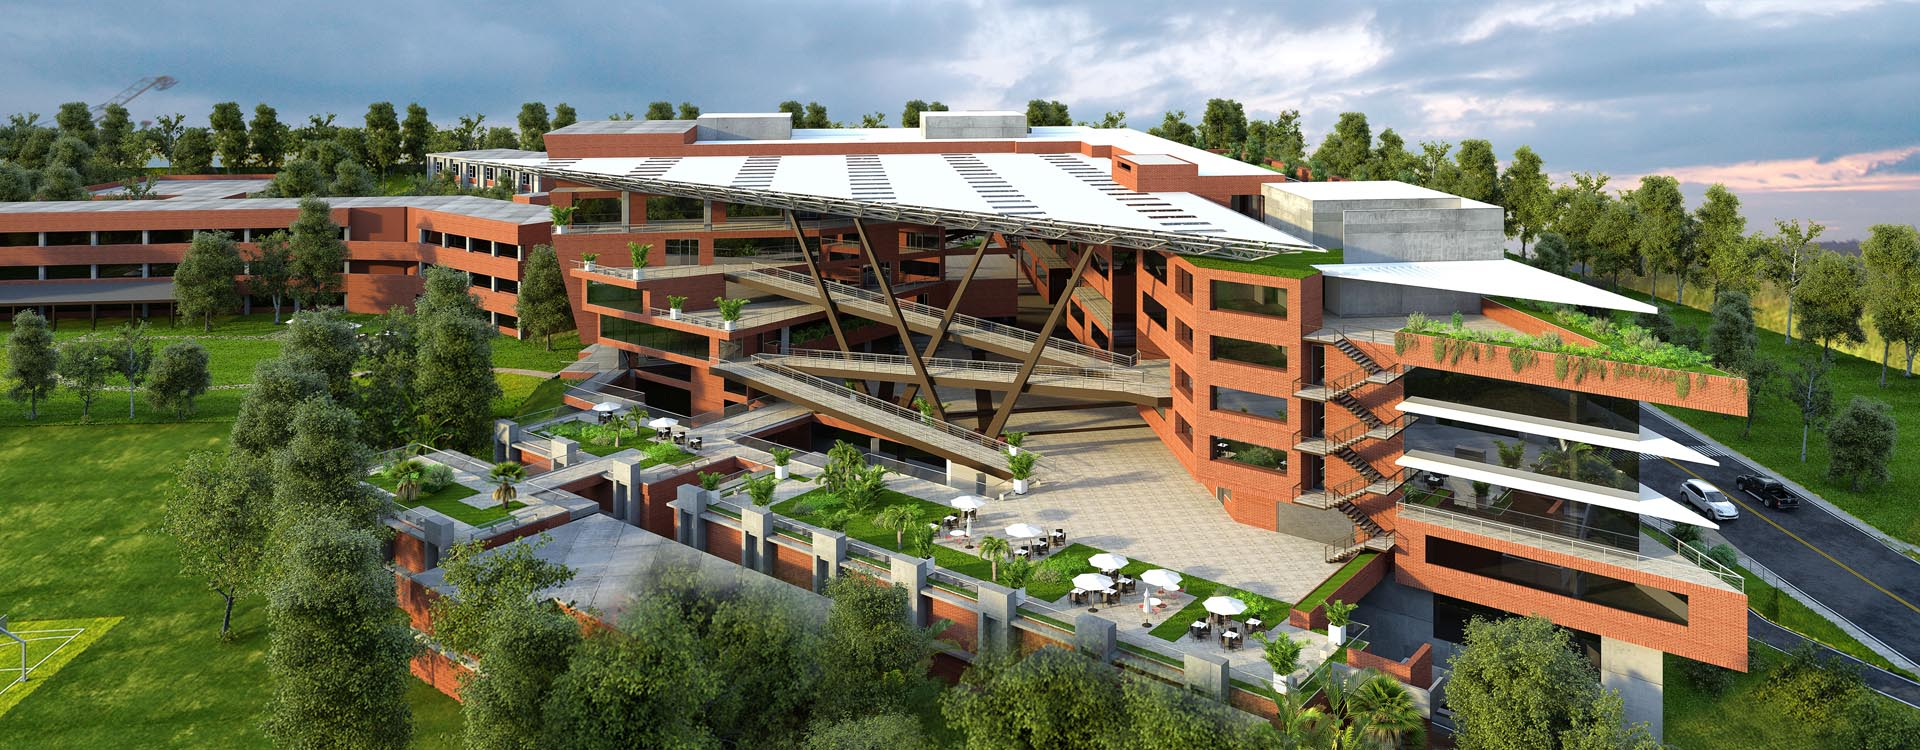
\includegraphics[height=13.25cm]{plantilla/portadacit.jpg}}
    	\makebox[\textwidth]{
    		\begin{overpic}[height=13.25cm]{\imagenportada}
     		\put(63,0){
\includegraphics[height=1.15in]{plantilla/fondologo_grande.png}}  
  			\put(64.5,2){
\includegraphics[height=0.55in]{plantilla/logoUVGblanco.eps}} 
        	\end{overpic}
    	}
    	%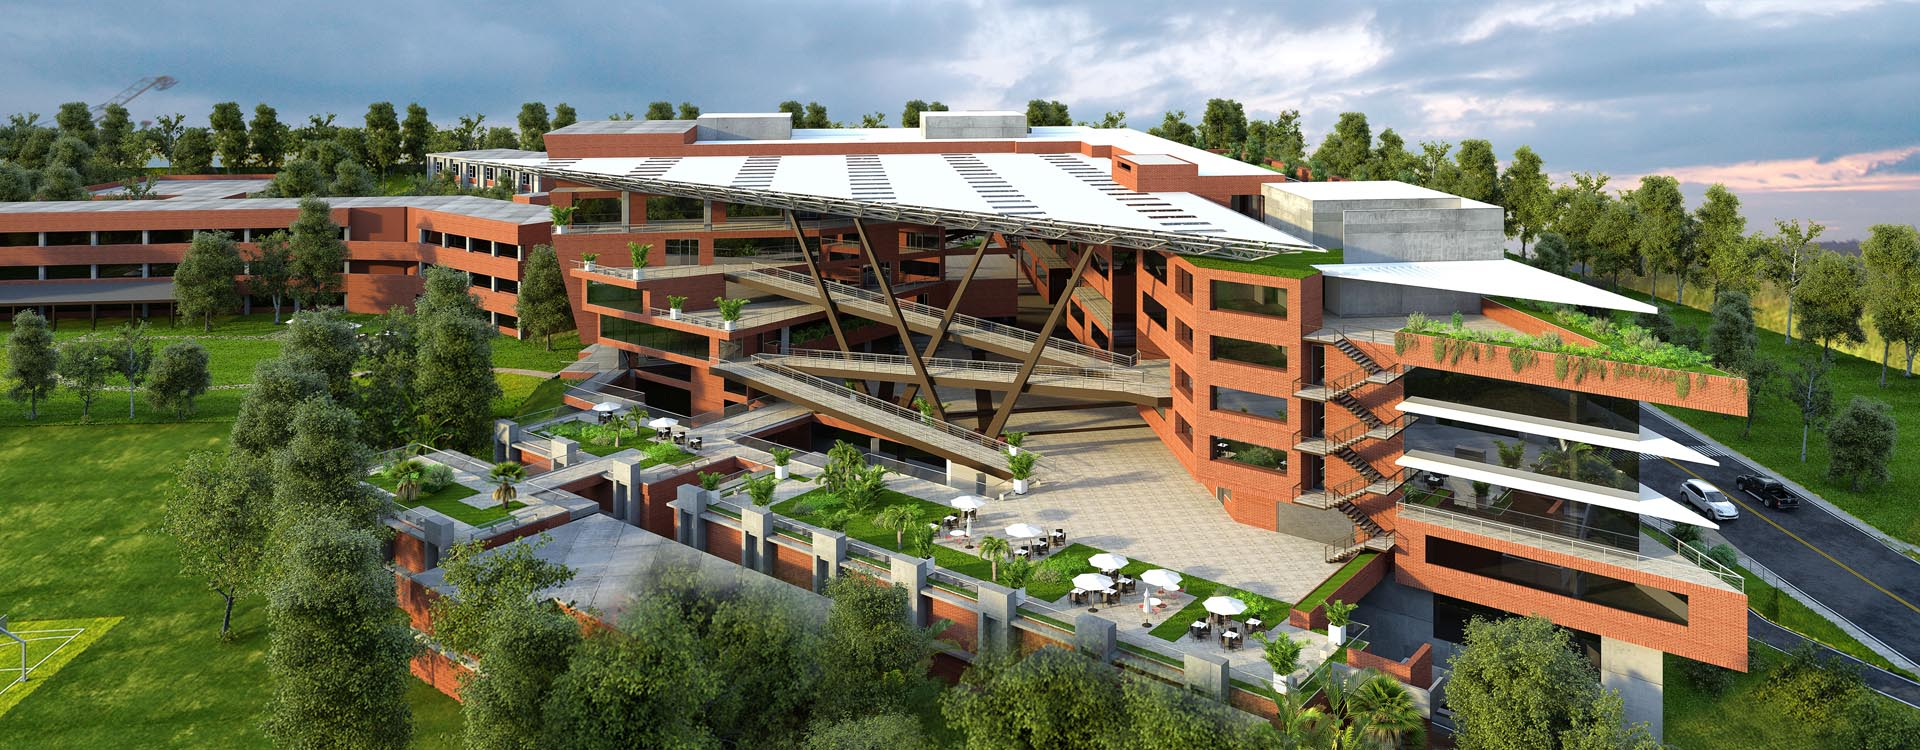
\includegraphics[height=13.25cm]{plantilla/portadacit.jpg}
	\end{figure}
	\restoregeometry
\fi

% ================================================================================
% PRIMERA PÁGINA
% ================================================================================

\newpage
\thispagestyle{empty}
\pagecolor{white}
\mbox{}
\newpage

\ifdefined\CAPcaratula
	\newpage
%     \cleardoublepage\phantomsection
%     \pdfbookmark{Carátula}{toc}
	\pagecolor{white}
	\color{black}
	\setcounter{page}{1}
	\pagenumbering{roman}
	\thispagestyle{empty}
	\begin{center}
		\LARGE UNIVERSIDAD DEL VALLE DE GUATEMALA\\
		\LARGE Facultad de \uvgfacultad \\[0.75cm]
	\end{center}
	\begin{figure}[h]
		\begin{center}
		
\includegraphics[height=5.5 cm]{plantilla/escudoUVGnegro.eps}
		\vspace{0.5in}
		\end{center}
	\end{figure}
	\begin{center}
		\LARGE \textbf{\titulotesis} \\
		\vfill
		\vfill
		\Large Trabajo de graduación en modalidad megaproyecto tecnológico presentado por \\
		\Large \nombreestudiante \\
		\Large Para optar al grado académico de Licenciado en \uvgcarrera \\
		\vfill
		\large Guatemala, \mesentrega del \anoentrega
	\end{center}
\fi

% ================================================================================
% HOJA DE FIRMAS
% ================================================================================

\newpage
\thispagestyle{empty}
\mbox{}
\newpage

\ifdefined\CAPfirmas
	\newpage
	\thispagestyle{empty}
	\vspace*{0.5in}
	\large Vo.Bo.:\\[1cm]
	\begin{center}
		(f) \rule[1pt]{4 in}{1pt}\\
		\nombreasesor
	\end{center}
	\vspace{1in}

	Tribunal Examinador:\\[1cm]
	\begin{center}
		(f) \rule[1pt]{4 in}{1pt}\\
		\nombreasesor \\[1in]
		(f) \rule[1pt]{4 in}{1pt}\\
		\nombreprimerex \\[1in]
		(f) \rule[1pt]{4 in}{1pt}\\
		\nombresegundoex
	\end{center}
	\vspace{1in}

	Fecha de aprobación: Guatemala, \fechaaprobacion.
	\normalsize
\fi

% ================================================================================
% CONTENIDO DEL TRABAJO
% ================================================================================
% PREFACIO
% --------------------------------------------------------------------------------

\newpage
\thispagestyle{empty}
\mbox{}
\newpage  

\ifdefined\CAPprefacio
	\newpage
	\cleardoublepage\phantomsection
    \chapter*{Prefacio}
    \ifdefined\parpordefecto
    	\defaultparformat{prefacio}
    \else
    	El proyecto \textit{Señas Chapinas: Traductor de Lensegua} nació de la necesidad de reducir las barreras de comunicación que enfrenta la comunidad sorda en Guatemala, quienes utilizan la lengua de señas guatemalteca, Lensegua, como principal medio de expresión. Esta iniciativa tuvo el propósito de ofrecer una solución tecnológica que permita traducir Lensegua a texto y voz en tiempo real, ayudando a la comunidad sorda a participar en la sociedad de una manera más equitativa y autónoma.

Mi contribución al proyecto se centra en el desarrollo de la infraestructura de red y la arquitectura de backend, componentes esenciales para asegurar la estabilidad, seguridad, y eficiencia de la plataforma. Esta arquitectura se concibe como el núcleo técnico del sistema, integrando y facilitando la comunicación entre todos los módulos de la aplicación, desde el procesamiento de lenguaje natural hasta la visión por computadora. El backend no solo habilita el funcionamiento del traductor de señas, sino que también provee la base para escalar el proyecto en el futuro, adaptándose a las necesidades crecientes de la comunidad y del equipo de desarrollo.

Quiero expresar mi sincero agradecimiento al Ing. Miguel Novella, quien me brindó apoyo y orientación en cada etapa de esta compleja infraestructura. También agradezco a la Universidad del Valle de Guatemala, así como a En-Señas Guatemala y ASEDES, por los recursos y respaldo necesario para alcanzar los objetivos planteados. Su apoyo hizo posible que los sistemas de comunicación y procesamiento de datos del proyecto tomaran forma en condiciones óptimas y en un entorno seguro.

A mi familia y amigos, gracias por su inagotable apoyo y por ser mi motivación constante a lo largo de este camino. Este proyecto no habría sido posible sin su confianza y aliento inquebrantable.
    \fi
    \addcontentsline{toc}{chapter}{Prefacio}
\fi

% AGRADECIMIENTOS
% --------------------------------------------------------------------------------

\newpage
\thispagestyle{empty}
\mbox{}
\newpage 

\ifdefined\CAPagradecimientos
	\newpage
    \cleardoublepage\phantomsection
	\chapter*{Agradecimientos}
	\ifdefined\parpordefecto
    	\defaultparformat{agradecimientos}
    \else
    	A mis seres queridos, mis padres por apoyarme en este camino y por creer en mi, a mi pareja por siempre darme alientos cuando mas lo necesitaba ayudarme y apoyarme en los momentos donde mas lo requeria.

Ingeniero Miguel Novella por estar pendiente y apoyarme como asesor, como docente y como profesional.

Ingeniero Erick por apoyarme en el levantamiento de forticlient en el sistema al inicio del proyecto y su apoyo en el intento de acceso al port forward.

Agradezco también a la Universidad del Valle de Guatemala y a las organizaciones En-Señas Guatemala y ASEDES por proporcionar el respaldo y los recursos necesarios para llevar a cabo esta investigación.

A T1 por mostrarme que hay que mantenerse fuerte y constante, que las batallas mas duras se pueden lograr.
    \fi 
	\addcontentsline{toc}{chapter}{Agradecimientos}
\fi

% ÍNDICE GENERAL
% --------------------------------------------------------------------------------

\newpage
\thispagestyle{empty}
\mbox{}
\newpage  

\ifdefined\CAPindice
	\newpage
    %\cleardoublepage\phantomsection
	\renewcommand{\contentsname}{Índice}
    \phantomsection
    \pdfbookmark{\contentsname}{toc}
	\tableofcontents
\fi

% LISTADO DE FIGURAS
% --------------------------------------------------------------------------------

\newpage
\thispagestyle{empty}
\mbox{}
\newpage  

\ifdefined\CAPfiguras
	\newpage
    \cleardoublepage\phantomsection
	\renewcommand{\listfigurename}{Lista de Figuras}
	\listoffigures
	\addcontentsline{toc}{chapter}{Lista de Figuras}
\fi

% LISTADO DE CUADROS
% --------------------------------------------------------------------------------

\newpage
\thispagestyle{empty}
\mbox{}
\newpage  

\ifdefined\CAPcuadros
	\newpage
    \cleardoublepage\phantomsection
	\renewcommand{\listtablename}{Lista de Cuadros}
	\listoftables
	\addcontentsline{toc}{chapter}{Lista de Cuadros}
\fi

% RESUMEN
% --------------------------------------------------------------------------------

\newpage
\thispagestyle{empty}
\mbox{}
\newpage  

\ifdefined\CAPresumen
	\newpage
    \cleardoublepage\phantomsection
	\chapter*{Resumen}
	\ifdefined\parpordefecto
		\defaultparformat{resumen}
	\else
		En este proyecto se desarrolló e implementó un servidor seguro y eficiente, capaz de administrar datos y soportar modelos avanzados de inteligencia artificial y visión por computadora. El principal objetivo fue crear una instancia de desarrollo que permitiera realizar despliegues, pruebas y ejecuciones de modelos de IA a través de un ambiente accesible para usuarios externos mediante APIs.

Para cumplir con estos objetivos, se configuraron máquinas virtuales, abriendo puertos para acceso remoto y desarrollando scripts de despliegue que facilitan la instalación y actualización de los modelos de IA. La infraestructura del servidor fue optimizada para manejar eficientemente grandes volúmenes de datos, con una arquitectura basada en Nginx y Gunicorn, respaldada por SQLAlchemy para la gestión de base de datos.

Las pruebas de carga y seguridad realizadas confirmaron la capacidad del sistema para operar bajo condiciones de alta demanda. Además, la evaluación de seguridad mediante Lynis mostró que el servidor cumple con estándares elevados, superando el objetivo de seguridad planteado. Este proyecto concluye que el servidor es adecuado para un entorno de producción, ofreciendo una plataforma estable y segura para el despliegue y gestión de aplicaciones de IA.
	\fi
	\addcontentsline{toc}{chapter}{Resumen}
\fi

% INTRODUCCIÓN
% --------------------------------------------------------------------------------

\newpage
\thispagestyle{empty}
\mbox{}
\newpage  

\ifdefined\CAPintroduccion
	\newpage
	\pagenumbering{arabic}
	\setcounter{page}{1}
	\chapter{Introducción}
	\ifdefined\parpordefecto
		\defaultparformat{introduccion}
	\else
		El objetivo central de este proyecto fue el desarrollo de una aplicación móvil que utilizó tecnología avanzada para la traducción en tiempo real de lengua de señas a texto y voz, facilitando así la comunicación para personas con discapacidad auditiva. Esta aplicación se valió de visión por computadora para detectar gestos y señas de manera efectiva y de tecnologías de inteligencia artificial para convertir estas señas a lenguaje natural, asegurando una interacción fluida y comprensible.

Adicionalmente, se diseñó una infraestructura de red dedicada que permitió no solo la comunicación efectiva entre la aplicación y el servidor central, sino también la gestión eficiente del flujo de datos. Esta infraestructura fue clave para recibir, procesar y responder a los videos enviados por los usuarios, implementando procesos que iban desde la interpretación de imagen hasta el procesamiento por modelos de inteligencia artificial, culminando con la entrega de la traducción al dispositivo del usuario.

Con el objetivo de hacer un proyecto accesible y que tuviera la oportunidad de crecer en el futuro, se buscó que la arquitectura de red y el servidor fueran seguros, eficientes y que tuvieran la capacidad de escalar. Esto se logró con el uso de APIs robustas y de máquinas virtuales que sirvieron para administrar el uso de recursos de la mejor manera posible.
	\fi
\fi

% OBJETIVOS
% --------------------------------------------------------------------------------

\newpage
\thispagestyle{empty}
\mbox{}
\newpage  

\ifdefined\CAPobjetivos
	\newpage
	\chapter{Objetivos}
	\ifdefined\parpordefecto
		\defaultparformat{objetivos}
	\else
		\section{Objetivo General}
\begin{itemize}
\item Desarrollar y desplegar un servidor que administre datos de forma segura y eficiente, optimizando el uso de recursos computacionales para soportar modelos de inteligencia artificial avanzados. 

\item Generar una instancia de desarrollo que posea las herramientas y facilidades para poder levantar, instalar, probar y ejecutar modelos de inteligencia artificial y visión por computadora.
\end{itemize}

\section{Objetivos Específicos}
\begin{itemize}
\item Crear un ambiente virtual que pueda ser accedido por usuarios externos, que les permita realizar deploys, pruebas y ejecuciones de diferentes modelos de inteligencias artificiales y de visión por computadora a través del uso de API’s.
\item Optimizar el proceso de recepción, almacenamiento y procesamiento de videos para múltiples usuarios, priorizando la eficiencia y reduciendo costos computacionales, medido a través de mejoras en tiempo de procesamiento, uso de recursos y costos operativos.
\item Fortalecer la seguridad para reducir el riesgo de robos de datos y ataques, buscando tener un valor de 4.0 en la escala de CVE (Common Vulnerabilities and Exposures) en el servidor.
\end{itemize}
	\fi
\fi

% JUSTIFICACIÓN
% --------------------------------------------------------------------------------

\newpage
\thispagestyle{empty}
\mbox{}
\newpage  

\ifdefined\CAPjustificacion
	\newpage
	\chapter{Justificación}
	\ifdefined\parpordefecto
		\defaultparformat{justificacion}
	\else
		En Guatemala, según datos del Conadi (Consejo Nacional para la Atención de las Personas con Discapacidad) recogidos hasta el mes de marzo del año 2021, existían entre 240,000 y 250,000 personas que utilizaban la lengua de señas como su principal herramienta de comunicación \cite{Conadi2021} . Sin embargo, el uso de esta lengua generaba barreras comunicativas entre una persona oyente y una persona sorda. Estas barreras limitaban la comunicación diaria de estas personas, restringiendo sus oportunidades e independencia.

Esta aplicación tuvo un enfoque especial en las frases de uso diario, preguntas, consultas y dudas que podían surgir en un día cotidiano, ya que estas personas enfrentaban muchos problemas para comunicarse en la realización de tareas cotidianas. Aunque estas tareas podían considerarse triviales para otros, para este sector representaban un reto significativo. Además, se buscó fomentar una mayor autonomía para estas personas, lo que les permitió una inserción más rápida, dinámica y amplia dentro del mundo laboral, facilitando así la obtención de una variedad más amplia de empleos.

También se destacaron las dificultades y barreras de lenguaje que podían ocasionar problemas más serios en situaciones delicadas y de alto estrés. Por ejemplo, en casos en los que las personas que usaban la lengua de señas enfrentaban grandes dificultades para escribir o comunicarse de cualquier otra forma que no fuera mediante esta lengua. Esto podía ocurrir en emergencias médicas, donde la obtención de información básica del paciente era imperativa, o en situaciones como un robo o la necesidad de pedir indicaciones o información bajo estrés, como al interactuar con un agente de policía. Estas son solo algunas de las muchas situaciones en las que las personas que necesitaban la lengua de señas podían encontrarse en una seria desventaja o en riesgo, lo que hacía que una comunicación óptima y la posibilidad de hacer y responder preguntas fueran de gran importancia.

Un aspecto fundamental de este proyecto fue la integración de los diferentes componentes tecnológicos para que trabajaran como una unidad cohesiva en lugar de entidades separadas. Esta integración tuvo una relevancia crítica, ya que permitió desarrollar un sistema que conecta las capacidades de los modelos de inteligencia artificial, la funcionalidad de la aplicación móvil y la infraestructura del servidor. La aplicación tenía como objetivo principal permitir a los usuarios grabar videos de personas utilizando LENSEGUA, enviar textos en español LENSEGUA, y proporcionar herramientas accesibles directamente en sus manos. Para lograr esto, fue indispensable contar con modelos sólidos para el procesamiento de datos, una aplicación intuitiva que sirviera como puente entre los usuarios y la tecnología, y un servidor robusto que facilitara la comunicación entre todos los componentes. Este enfoque integral no solo garantizó la efectividad del sistema, sino que también aseguró su escalabilidad y capacidad para atender las necesidades reales de la comunidad sorda.

\begin{figure}[H]
    \centering
    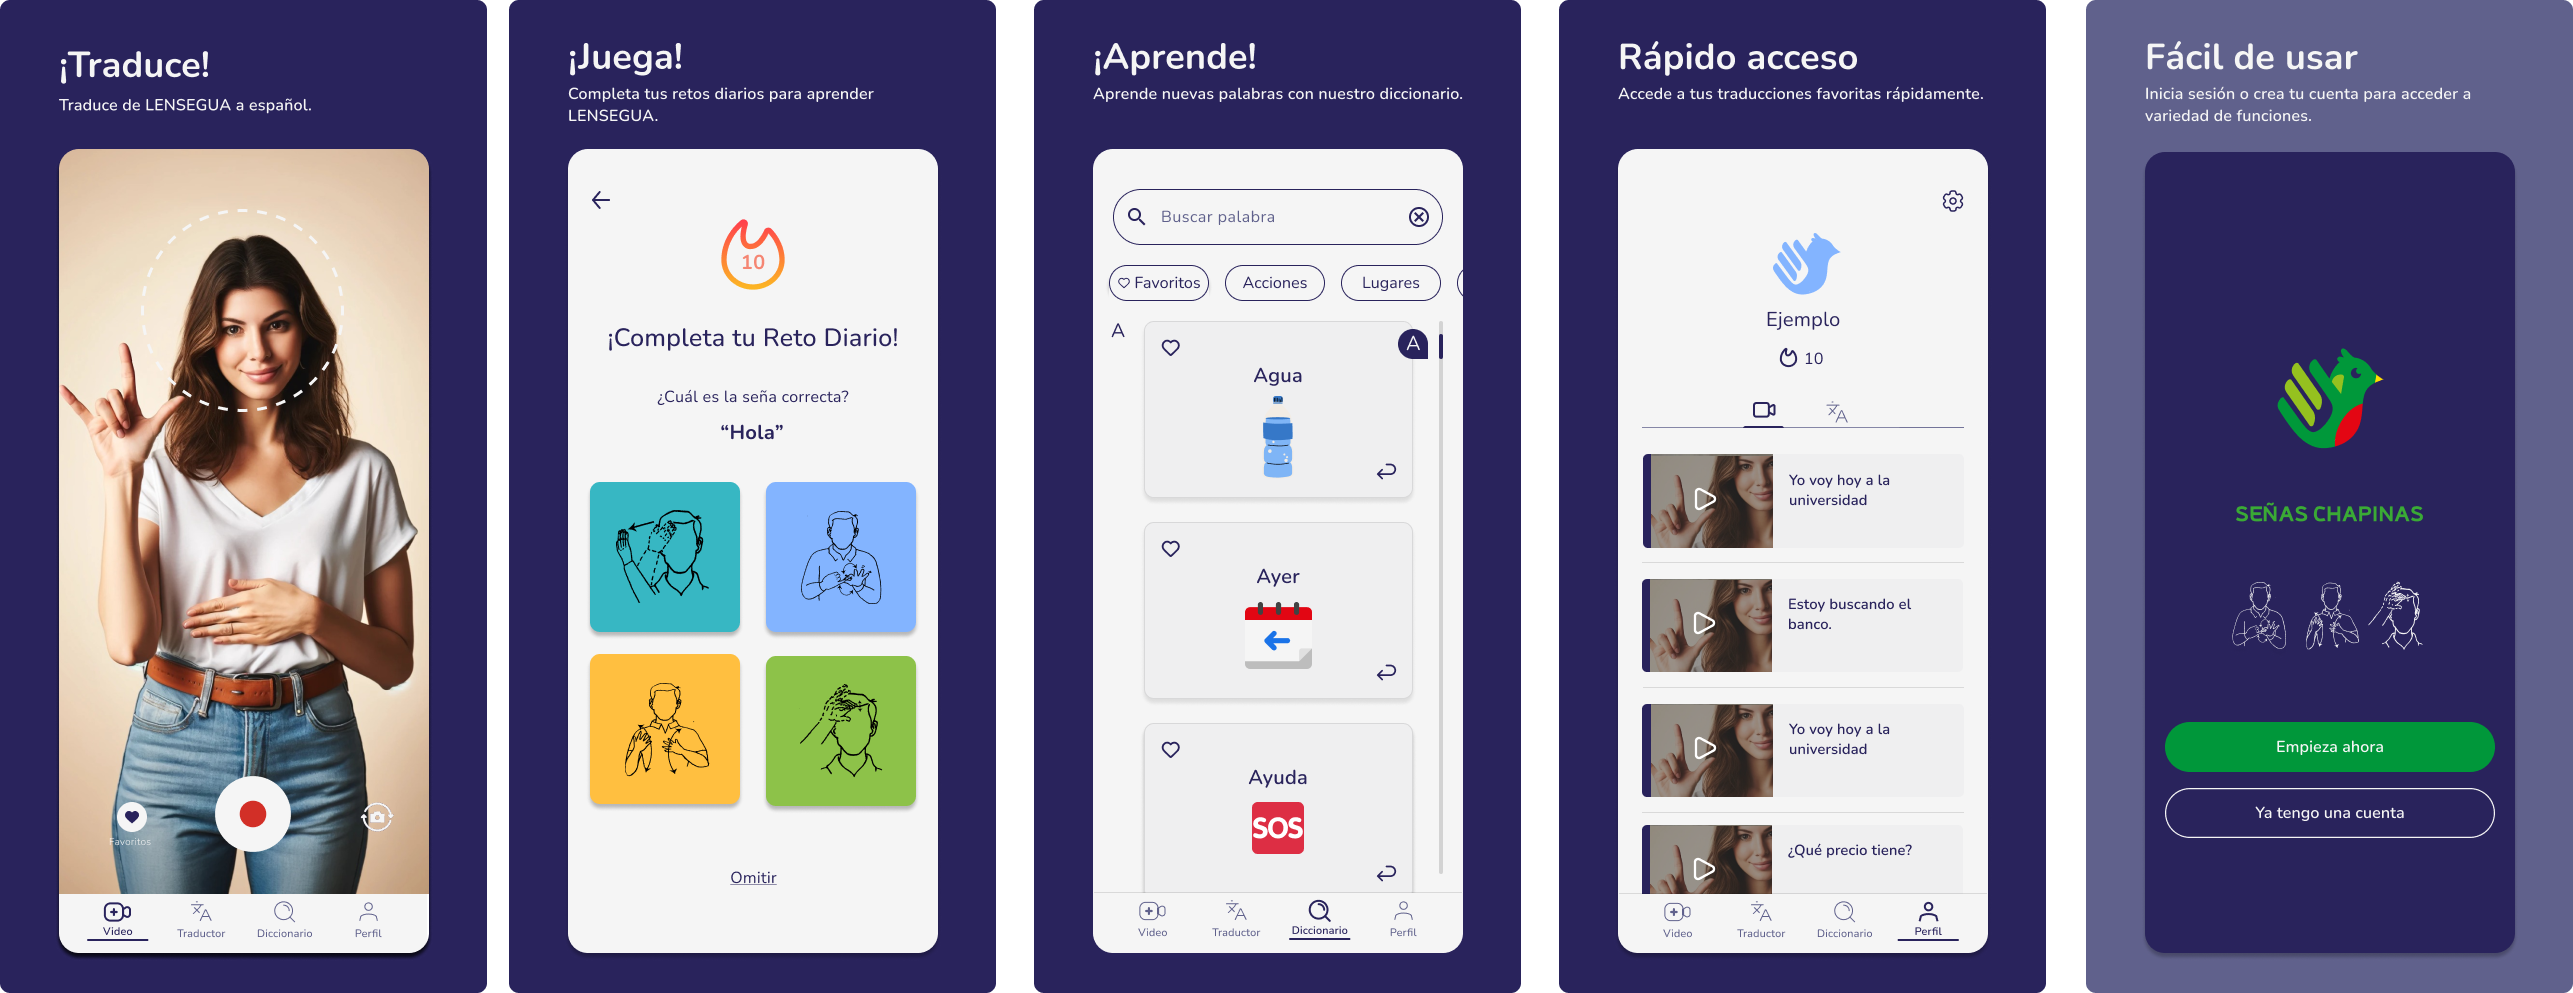
\includegraphics[width=0.5\textwidth]{figuras/capturas_app.png}
    \caption{Aplicación: Señas Chapinas.}
    \label{fig:capturas_app}
\end{figure}
	\fi
\fi

% MARCO TEÓRICO
% --------------------------------------------------------------------------------

\newpage
\thispagestyle{empty}
\mbox{}
\newpage  

\ifdefined\CAPmarcoteorico
	\newpage
	\chapter{Marco Teórico}
	\ifdefined\parpordefecto
		\defaultparformat{marco_teorico}
	\else
		\section{Lensegua}

\subsection{¿Qué es Lensegua?}
En Guatemala, el Lenguaje de Señas Guatemalteco (Lensegua) se oficializó el 18 de febrero de 2020 con el Decreto 3-2020. Este decreto regula la aprobación, desarrollo, uso y fomento de Lensegua, asegurando su reconocimiento y promoción en el país. 

``Lengua de señas de Guatemala. Es la lengua oficial para poder comunicarse en lengua de señas en Guatemala (según Decreto 3-2020)" \cite{Lensegua}.

\subsection{Historia de Lensegua}
En Guatemala, la comunidad sorda comenzó a desarrollar sus propios signos y métodos de comunicación, adaptando movimientos, posiciones y representaciones de letras a sus necesidades culturales y sociales. Este proceso fue orgánico, impulsado por la interacción diaria y la necesidad de comunicación efectiva dentro de la comunidad.

El reconocimiento oficial de Lensegua llegó el 18 de febrero de 2020, con la promulgación del Decreto 3-2020. Este decreto estableció la regulación para la aprobación, desarrollo, uso y fomento de la Lengua de Señas de Guatemala. Con esta legislación, el gobierno guatemalteco no solo reconoció la importancia de Lensegua, sino que también se comprometió a promover su enseñanza y uso en todo el país, asegurando que la comunidad sorda tenga acceso a una forma de comunicación efectiva y respetada. La implementación de Lensegua ha sido un hito significativo para la inclusión y el reconocimiento de los derechos de las personas sordas en Guatemala, marcando un paso crucial hacia una sociedad más inclusiva y equitativa \cite{LenseguaHistoria}.

\section{Sistema Operativo: Linux Server}

\subsection{¿Qué es Linux?}
Linux es un sistema operativo de código abierto basado en Unix que se ha establecido como una opción poderosa y versátil para una variedad de plataformas, desde servidores y supercomputadoras hasta dispositivos móviles y electrodomésticos. Fue creado inicialmente por Linus Torvalds en 1991. El núcleo de Linux, conocido como el kernel, gestiona las interacciones del software con el hardware y es vital para la regulación de los recursos del sistema. A lo largo de los años, Linux ha ganado una popularidad masiva, en parte debido a su naturaleza de código abierto, que permite a los usuarios modificar y mejorar su software según necesiten. Además, su alta configurabilidad, estabilidad y robustez en seguridad lo hacen preferido en entornos empresariales y académicos. La comunidad de Linux es una de sus mayores fortalezas, contribuyendo constantemente con una amplia gama de distribuciones adaptadas a diferentes usos y preferencias \cite{Linux}.

\subsection{Historia de Linux}
Linux es un sistema operativo de código abierto creado en 1991 por Linus Torvalds, un estudiante de la Universidad de Helsinki. Inspirado en Unix, Torvalds deseaba ofrecer una alternativa gratuita y accesible, por lo que liberó Linux bajo la Licencia Pública General de GNU para permitir su uso, modificación y redistribución libre. Inicialmente adoptado por entusiastas tecnológicos y desarrolladores, Linux ha evolucionado hasta ser ampliamente utilizado en servidores, dispositivos móviles y supercomputadoras. Destacado por su estabilidad, seguridad y flexibilidad, es ahora uno de los sistemas operativos más predominantes a nivel mundial, con múltiples distribuciones como Ubuntu, Fedora y Arch que facilitan su uso en una gran variedad de entornos \cite{HistoriaLinux}.

\subsection{Linux Server}
Un servidor Linux se compone fundamentalmente de Linux, una familia de sistemas operativos de software libre y código abierto que se desarrollan alrededor del kernel de Linux. Originalmente creado como una versión alternativa y libre del sistema operativo MINIX, los servidores Linux se han popularizado gracias a su estabilidad, seguridad y flexibilidad. Estas características no solo los diferencian de sus contrapartes propietarias, sino que también mantienen bajos los costos de configuración y mantenimiento. Además, ofrecen una flexibilidad aumentada en la configuración, operación y mantenimiento de un servidor. Un sistema operativo de servidor Linux proporciona la interfaz central para la gestión de usuarios e implementa diversos servicios de seguridad y administración, todos cruciales para operar en una arquitectura cliente-servidor \cite{LinuxServer}.

\section{Virtualización}
La virtualización, en el contexto de la computación, implica la creación de versiones virtuales de recursos que originalmente eran físicos, como sistemas operativos y hardware de red. Este proceso permite a un solo servidor físico alojar múltiples máquinas virtuales (VMs), cada una con su propio sistema operativo y aplicaciones, operando de manera independiente pero compartiendo los recursos subyacentes del hardware físico \cite{Virtualizacion}.

El propósito principal de la virtualización fue maximizar la eficiencia del uso de recursos al permitir que múltiples sistemas operativos y aplicaciones se ejecutaran en un solo servidor físico. Esto no solo reduce los costos de hardware, sino que también aumenta la flexibilidad y la escalabilidad de los sistemas de TI. Las VMs pueden migrar entre servidores con mínimo tiempo de inactividad, lo que facilita el mantenimiento y la gestión del sistema \cite{Virtualizacion2}.

\section{Multipass}
Multipass es una herramienta ligera de virtualización diseñada para facilitar la creación y gestión de máquinas virtuales, enfocada especialmente en entornos de desarrollo y pruebas rápidas. Al integrarse de manera nativa con Ubuntu, Multipass permite desplegar y administrar múltiples instancias de Linux de manera eficiente, actuando como una mini-nube local en tu propio equipo. Multipass ha sido desarrollado con la simplicidad en mente, proporcionando una experiencia optimizada para usuarios que necesitan acceder rápidamente a entornos virtuales consistentes sin la complejidad de configuraciones avanzadas \cite{Multipass}.

\section{VPN}
\subsection{¿Qué es una VPN?}
Una VPN (red privada virtual) establece una conexión segura y privada entre dispositivos a través de Internet. Este tipo de red es fundamental para la transmisión de datos de manera segura y anónima a través de infraestructuras públicas. El proceso implica enmascarar las direcciones IP de los usuarios y cifrar la información transmitida, asegurando que solo las partes autorizadas puedan acceder y leer estos datos \cite{VPN}.

\subsection{¿Para qué sirven las VPNs?}
Las VPNs, o redes privadas virtuales, son esenciales para permitir conexiones remotas seguras a servidores y recursos de red. OpenVPN, un destacado software de VPN de código abierto, facilitó el establecimiento de redes locales virtuales entre computadoras dispersas geográficamente, permitiendo a los usuarios acceder y operar servidores y datos como si estuvieran físicamente presentes en la misma red local. Esto es crucial para empresas y organizaciones con equipos distribuidos, asegurando que la comunicación y el acceso a recursos críticos sean seguros y eficientes \cite{OpenVPN}.

\section{Arquitectura de base de datos}
\subsection{Bases de datos relacionales}
Una base de datos relacional es una estructura que organiza la información en filas y columnas dentro de tablas, facilitando el almacenamiento, la búsqueda y la gestión de datos de manera eficiente. Las tablas se enlazan entre sí mediante claves primarias y claves foráneas, creando relaciones que reflejan cómo se conectan los datos en diferentes tablas. Este sistema permite a los usuarios emplear consultas SQL para cruzar información de diversas tablas, proporcionando una herramienta poderosa para analizar y resumir el rendimiento empresarial \cite{Relacionales}.

\subsection{PostgreSQL}
PostgreSQL es una mejora del sistema de gestión Postgres, un prototipo avanzado de DBMS de próxima generación. Mientras conserva el modelo de datos potente y los tipos de datos ricos de Postgres, PostgreSQL ha reemplazado el lenguaje de consulta POSTQUEL por un subconjunto extendido de SQL, convirtiéndolo en una opción gratuita y de código abierto para el manejo de bases de datos. Desarrollado inicialmente en la Universidad de California en Berkeley, PostgreSQL ha evolucionado significativamente gracias a la contribución de un equipo de desarrolladores a nivel mundial \cite{Postgres}.

\subsection{Arquitectura de base de datos}
La arquitectura de datos se refiere al diseño estructural y a la metodología empleada para organizar y gestionar los recursos de datos en una organización o sistema. Este marco establece las políticas, normas y procedimientos para la recopilación, almacenamiento, manejo y uso de los datos con el fin de asegurar su accesibilidad, consistencia, integridad y seguridad. Una arquitectura de datos eficaz apoya la estrategia de información de una empresa, facilitando la integración y la operación de sistemas de TI, mejorando el soporte para las decisiones basadas en datos y optimizando el rendimiento de las aplicaciones \cite{ArquitecturaDatos}.

\section{APIs}
\subsection{¿Qué es una API?}
Una API (Interfaz de Programación de Aplicaciones) es un conjunto de reglas y especificaciones que las aplicaciones pueden seguir para comunicarse entre sí. Funciona como un puente que permite la interacción entre diferentes piezas de software de manera estandarizada. Por ejemplo, una aplicación de pronóstico del tiempo puede recibir datos de un servicio meteorológico utilizando una API para comunicarse con el sistema de dicho servicio \cite{API}.

\subsection{¿Cómo usar una API?}
Usar una API a nivel básico implica interactuar con un conjunto de definiciones y protocolos que permiten la comunicación entre diferentes componentes de software. Primero, es esencial entender los métodos estándar que la API ofrece, como obtener, crear, actualizar o eliminar recursos. Cada interacción sigue un patrón predefinido, facilitando así la integración y uso de la API en proyectos \cite{UsoAPI}.

\subsection{Implementar APIs a bases de datos}
Al desarrollar una aplicación que necesite interactuar con una base de datos mediante una API, puedes realizar operaciones como crear, recuperar, actualizar o eliminar registros. Estas operaciones se definen claramente con ciertos parámetros de entrada esperados y formatos de respuesta, lo que facilita la integración de sistemas complejos \cite{ImplementarAPI}.

\subsection{Implementar APIs para recepción y devolución de datos}
El uso de una API para enviar y recibir información implica interacciones estructuradas mediante solicitudes y respuestas definidas. Un ejemplo común es usar un método HTTP POST para enviar datos a la API, que luego devuelve una respuesta indicando éxito o fallo \cite{ImplementarAPIDatos}.

\subsection{¿Qué es Crontab?}
`Crontab` es una herramienta en sistemas Unix/Linux que permite la programación de tareas automatizadas que se ejecutan a intervalos específicos. Estas tareas, conocidas como cron jobs, son útiles para ejecutar scripts y comandos de forma recurrente sin intervención manual, lo cual es ideal para tareas de mantenimiento o procesamiento automatizado, como el reinicio de rachas en nuestra aplicación \cite{HostingerCrontabTutorial}.

\section{Bases de diseño y filosofía de DARPA}
Entre los conceptos fundamentales aplicados en el diseño de la arquitectura del sistema, se adoptaron varios principios expuestos en el documento "The Design Philosophy of the DARPA Internet Protocols" \cite{DARPA}. A continuación, se destacan los siguientes conceptos clave:

\subsection{Costo-efectividad y control}
La arquitectura de Internet, según lo planteado por DARPA, enfatiza la necesidad de manejar los recursos de manera eficaz bajo control administrativo distribuido. Esto justifica la decisión de utilizar servidores propios en lugar de servicios en la nube para este proyecto, reduciendo dependencias externas y costos operativos. Al mantener un control directo sobre la infraestructura, se puede gestionar de manera más eficiente el uso de los recursos, optimizando la relación costo-beneficio sin sacrificar el rendimiento.

\subsection{Flexibilidad y adaptabilidad}
La filosofía de diseño también subraya la importancia de adaptarse a diferentes entornos y requisitos técnicos. En este proyecto, la elección de Ubuntu como sistema operativo refleja un compromiso con un sistema flexible y robusto, ya que permite una personalización extensa. Aunque inicialmente se consideró el uso de RAID para la gestión del almacenamiento, se decidió desinstalarlo y desconfigurarlo debido a las limitaciones específicas del entorno de este proyecto. Esto asegura que la infraestructura sea adaptable a las necesidades actuales, manteniendo un enfoque simplificado en la gestión de recursos.

\subsection{Seguridad y privacidad}
Siguiendo los principios de diseño de DARPA, la seguridad es una prioridad fundamental. La integridad y seguridad de la comunicación entre los sistemas es vital para el éxito del proyecto. En este sentido, la implementación de una VPN segura mediante OpenVPN garantiza la protección de los datos transmitidos, asegurando que el acceso remoto y la transferencia de información se realicen de manera segura y confiable, reduciendo el riesgo de vulnerabilidades y ataques.

\section{Pruebas de eficiencia y de extremo a extremo en el servidor mediante APIs}

\subsection{¿Qué es una prueba de eficiencia?}
Las pruebas de eficiencia miden cómo el servidor responde bajo condiciones de carga habitual, evaluando aspectos como el tiempo de respuesta, la utilización de recursos (CPU, memoria y disco), y la capacidad del sistema para gestionar solicitudes simultáneas sin afectar negativamente el rendimiento. Estas pruebas permiten identificar oportunidades de optimización y ajustar la infraestructura para garantizar un rendimiento óptimo en condiciones normales de operación \cite{E2ETestingOverview}.

\subsection{¿Qué es una prueba de extremo a extremo (E2E)?}
Las pruebas de extremo a extremo (E2E) verifican el funcionamiento integral de la aplicación, evaluando cómo interactúan todos sus componentes en un flujo completo desde el punto de vista del usuario. Estas pruebas son esenciales para asegurarse de que cada parte de la aplicación, incluidas las APIs, funcione como se espera y que todos los puntos de interacción respondan adecuadamente dentro del sistema.

\begin{itemize}
    \item \textbf{Objetivo:} Confirmar que todas las partes de la aplicación operan de manera integrada, verificando que los flujos de trabajo completos (como registro, autenticación, envío de datos y consulta de información) se ejecuten sin errores.
    \item \textbf{Resultado esperado:} Que la aplicación realice todas las operaciones y flujos clave sin problemas, asegurando que cada funcionalidad principal esté correctamente integrada y funcione en conjunto.
\end{itemize}

\subsection{Impacto de la eficiencia y de las pruebas de extremo a extremo en el servidor}

\begin{itemize}
    \item \textbf{Eficiencia:} Un servidor eficiente maximiza el uso de los recursos disponibles, lo que permite reducir los costos operativos y mantener un rendimiento constante. Esto es esencial para asegurar tiempos de respuesta rápidos y garantizar que el sistema pueda manejar múltiples solicitudes concurrentes sin una degradación del servicio.

    \item \textbf{Pruebas E2E:} Las pruebas de extremo a extremo permiten validar el flujo completo de operaciones, asegurando que cada componente del sistema funcione correctamente y en sincronía. Estas pruebas ayudan a identificar cualquier posible problema de integración entre APIs y otros módulos de la aplicación, lo que es esencial para una experiencia de usuario fluida y un sistema robusto.
\end{itemize}

\section{Herramientas para pruebas de eficiencia y de extremo a extremo}

Para realizar las pruebas de eficiencia y extremo a extremo, se emplearon las siguientes herramientas:

\begin{itemize}
    \item \textbf{Python:} Se utilizó para desarrollar scripts personalizados que permiten simular múltiples usuarios y escenarios de carga en la aplicación, evaluando el tiempo de respuesta, el rendimiento y el uso de recursos en situaciones de carga típica y bajo prueba de integración completa \cite{PythonTesting}.
    \item \textbf{NGINX Amplify:} Herramienta de monitoreo utilizada para supervisar el uso de recursos en tiempo real, como CPU, memoria y tráfico de red. NGINX Amplify proporciona métricas detalladas y facilita el análisis de rendimiento durante las pruebas, identificando posibles áreas de optimización y problemas de integración \cite{NGINXAmplifyMonitoring}.
\end{itemize}

\subsection{Monitoreo del sistema}
\begin{itemize}
    \item \textbf{htop}: Proporciona una vista en tiempo real del uso de CPU, memoria y procesos en ejecución.
    \item \textbf{dstat}: Genera estadísticas combinadas de CPU, disco, memoria y red.
    \item \textbf{iotop}: Muestra el uso de disco por cada proceso, facilitando la identificación de procesos que consumen muchos recursos.
    \item \textbf{Prometheus}: Sistema de monitorización para métricas a gran escala.
    \item \textbf{Prometheus-Exporter}: Herramienta para monitorear las solicitudes entrantes al servidor.
    \item \textbf{Grafana}: Plataforma de visualización de métricas, utilizada para analizar los resultados de Prometheus \cite{MonitoringTools}.
\end{itemize}

\subsection{Pruebas de carga y end to end}

Las pruebas de carga se centran en medir la respuesta del sistema bajo condiciones de uso previstas, simulando múltiples usuarios y solicitudes simultáneas. Estas pruebas permiten evaluar el rendimiento, tiempos de respuesta y estabilidad del sistema cuando procesa diversas acciones en paralelo \cite{LoadViewLoadTesting}.

\begin{itemize} 
\item \textbf{Objetivo:} Evaluar cómo responde el sistema bajo una carga esperada de usuarios o solicitudes simultáneas, enfocándose en el rendimiento y la estabilidad mientras se procesan múltiples acciones. \item \textbf{Resultado esperado:} Que el sistema mantenga tiempos de respuesta y niveles de rendimiento aceptables bajo condiciones de uso normales (es decir, el número máximo de usuarios esperados en condiciones típicas). 
\item \textbf{Prueba:} La prueba de carga implementada simula a varios usuarios ejecutando operaciones simultáneas, como autenticación, envío de videos y marcación de favoritos. Se registra el tiempo de respuesta y el estado de cada acción, evaluando así la capacidad de la aplicación para manejar un volumen esperado de usuarios sin degradar su rendimiento. 
\end{itemize}

Las pruebas de Extremo a Extremo (E2E) se orientan a evaluar el flujo completo de la aplicación desde la perspectiva del usuario. A diferencia de las pruebas de carga, estas pruebas verifican que todos los componentes del sistema funcionen conjuntamente como se espera en un caso de uso completo.

\begin{itemize} 
\item \textbf{Objetivo:} Confirmar que todas las partes de la aplicación funcionan de manera integrada y que los componentes interactúan correctamente en un flujo de uso completo. \item \textbf{Resultado esperado:} Que la aplicación ejecute todas las operaciones y flujos clave sin errores (por ejemplo, registro, autenticación, envío y consulta de datos), asegurando que las funcionalidades principales se integren de manera adecuada. 
\item \textbf{Prueba:} La prueba E2E implementada cubre un caso de uso completo, desde la creación de un usuario hasta la interacción con las principales funciones de la aplicación, como autenticación, carga de videos, traducción y manipulación de favoritos. Esta prueba garantiza que cada parte del sistema funcione en conjunto en el flujo real de un usuario. 
\end{itemize}

\section{Trabajo de campo}
Durante el proyecto, se tomó la decisión de no utilizar servicios en la nube como AWS o Azure debido al alto costo de sus equipos y servicios. En su lugar, se optó por utilizar los servidores disponibles en la UVG, específicamente el modelo DELL R740 ubicado en Jack’s Cave. Este equipo, que no poseía un sistema operativo preinstalado, fue configurado con Ubuntu Server 22.08, elegido por su versatilidad y disponibilidad gratuita. Este sistema operativo permitió la implementación de múltiples herramientas, incluyendo VPNs mediante OpenVPN siguiendo los pasos proporcionados por DigitalOcean \cite{digitalocean_openvpn}, lo que facilitaron el acceso remoto seguro al servidor.

El proceso de instalación incluyó la interacción con el controlador de RAID del servidor, el cual estaba gestionado por el controlador DELL PERC. Aunque RAID permite gestionar múltiples discos duros de manera eficiente, en este caso específico, donde solo se dispone de un disco duro de 1.92 TB, se decidió no utilizar el controlador RAID, ya que no ofrecía ventajas significativas para el sistema. En su lugar, el disco duro fue gestionado directamente, implementando mejoras manuales que ofrecían un rendimiento adecuado sin la complejidad adicional de RAID \cite{Raid}.

Tras la instalación del sistema operativo, se procedió a configurar OpenVPN para gestionar el acceso remoto al servidor. Los pasos seguidos incluyeron:
1. Generación y configuración de los materiales criptográficos necesarios, como claves y certificados, para garantizar una comunicación segura entre el servidor y los clientes.
2. Ajuste de la configuración de red de OpenVPN para la correcta distribución del tráfico de datos.
3. Configuración de las reglas de firewall necesarias para permitir el tráfico a través de la VPN sin comprometer la seguridad del sistema.
4. Inicio del servicio de OpenVPN y realización de pruebas para asegurar que las conexiones remotas funcionen correctamente \cite{OpenVPNSetup}.


	\fi
\fi

% ANTECEDENTES
% --------------------------------------------------------------------------------

\newpage
\thispagestyle{empty}
\mbox{}
\newpage  

\ifdefined\CAPantecedentes
	\newpage
	\chapter{Antecedentes}
	\ifdefined\parpordefecto
    	\defaultparformat{antecedentes}
    \else
    	No existen antecedentes específicos en la Universidad sobre proyectos previos que integren de forma directa la arquitectura universitaria con el fin de acceder a un servidor dedicado para pruebas y desarrollo de modelos de inteligencia artificial y visión por computadora. Este proyecto representa el primer esfuerzo en crear un ambiente accesible y seguro para el despliegue de modelos avanzados, permitiendo el acceso externo mediante una infraestructura de servidores segura y controlada.

Sin embargo, se puede mencionar como antecedente cercano el proyecto titulado \textit{Plataforma para el registro, visualización y difusión de competencias educativas para la mejora en el proceso de reclutamiento laboral de los miembros del departamento de computación de la UVG}, desarrollado por Paul De Jesús Belches Flores-Gómez y David Uriel Soto Alvarez. Este proyecto tiene una orientación hacia el uso de APIs para la centralización y gestión de competencias educativas en la Universidad, mejorando el acceso a la información y facilitando su uso en contextos administrativos y de reclutamiento laboral.

A nivel administrativo, el proyecto de Belches y Soto estableció un precedente en el uso de tecnologías API para centralizar y organizar datos en la Universidad, sentando una base técnica que influyó en el planteamiento de este proyecto al buscar una integración efectiva de APIs en el entorno universitario.

Por otro lado, el profesor Miguel Novella jugó un rol importante en apoyar los esfuerzos para establecer un acceso seguro a la arquitectura universitaria, un proceso que involucró la colaboración con el equipo de IT de la Universidad. Su experiencia y respaldo fueron esenciales en la gestión de permisos y en el acceso a la infraestructura universitaria, sentando las bases necesarias para la implementación exitosa del presente proyecto.

    \fi  
\fi

% ALCANCE
% --------------------------------------------------------------------------------

\newpage
\thispagestyle{empty}
\mbox{}
\newpage  

\ifdefined\CAPalcance
	\newpage
	\chapter{Alcance}
	\ifdefined\parpordefecto
    	\defaultparformat{alcance}
    \else
    	Este proyecto se desarrollará dentro de los límites de la infraestructura universitaria disponible, cumpliendo con los objetivos propuestos y permitiendo la ejecución de todas las funciones del servidor bajo las restricciones del entorno técnico de la Universidad. Los alcances abarcan tanto la capacidad de respuesta como la conexión segura para los usuarios de la aplicación, quienes deberán acceder al servidor a través de la VPN institucional FortiClient o desde la red local en el área conocida como la Jack's Cave, donde se encuentra físicamente ubicado el equipo.

Dada la restricción en la configuración de red y la falta de soporte para port-forwarding al exterior de la Universidad, se define que las conexiones externas no podrán realizarse sin acceso previo a la VPN universitaria o sin una conexión local directa al servidor. Esto introduce una capa adicional en el proceso de conexión, lo cual puede tener un impacto en la eficiencia de respuesta del sistema debido a la latencia introducida por la VPN.

Además, el proyecto está limitado al uso del equipo proporcionado en las instalaciones de la Universidad. Dado que no fue posible realizar expansiones o modificaciones en el hardware disponible, la infraestructura actual impone un límite en la escalabilidad del sistema. Este proyecto, por lo tanto, se ha diseñado cuidadosamente para optimizar el rendimiento dentro de los recursos de procesamiento, almacenamiento y red que el equipo de la Universidad permite.

Las pruebas de seguridad realizadas en este proyecto se enfocaron exclusivamente a nivel de software debido a que el servidor utilizado formaba parte de la infraestructura de la universidad, la cual contaba con políticas y configuraciones de seguridad preestablecidas que no estuvieron bajo nuestro control directo. Estas condiciones limitaron las mejoras adicionales que pudimos implementar a nivel de hardware o configuraciones específicas. Sin embargo, el enfoque en software fue válido, ya que según el NIST Cybersecurity Framework \cite{NISTCybersecurityFramework}, la mayoría de las vulnerabilidades críticas en servidores están relacionadas con configuraciones y software, no con el hardware. Además, este diseño aseguró que el sistema pudiera ser trasladado a otros servidores en el futuro, manteniendo la robustez de las medidas implementadas sin depender de un entorno físico específico. Herramientas como Lynis fueron diseñadas para evaluar y garantizar un nivel adecuado de seguridad en sistemas que podían operar en entornos diversos, haciendo este enfoque flexible y alineado con estándares modernos de seguridad.

\section{Consideraciones adicionales}

\begin{enumerate}
    \item \textbf{Seguridad y restricciones de acceso:} Las pruebas de acceso remoto estarán sujetas a las políticas de seguridad de la Universidad, limitándose al entorno universitario, lo cual asegura un control estricto sobre los datos y recursos.
  
    \item \textbf{Pruebas de carga y estrés limitadas al entorno interno:} Las evaluaciones de eficiencia y respuesta se basarán en simulaciones dentro del sistema de la Universidad, dado que la infraestructura no se encuentra abierta al público externo. Esto limita las pruebas a las condiciones internas del entorno universitario, lo cual deberá tenerse en cuenta para futuras escalas de uso.
  
    \item \textbf{Conformidad con los recursos de red de la Universidad:} Debido a la dependencia de la red de la Universidad, el rendimiento del servidor está condicionado a la calidad de la conexión local y a la estabilidad de la VPN, factores externos que pueden influir en la velocidad y confiabilidad del sistema.
  
    \item \textbf{Limitación en las pruebas de carga por duración del video:} Debido a la naturaleza del modelo y el material disponible, las pruebas de carga se realizaron exclusivamente con videos de una duración de 2 segundos.
\end{enumerate}

Estas precisiones establecen claramente el alcance dentro de los recursos disponibles y el entorno controlado de la Universidad, asegurando que el proyecto funcione de manera efectiva bajo las condiciones actuales y anticipando limitaciones para posibles expansiones o cambios futuros.

    \fi 
\fi

% CAPÍTULOS
% --------------------------------------------------------------------------------

\newpage
\thispagestyle{empty}
\mbox{}
\newpage  

\newpage
\ifdefined\parpordefecto
	\defaultparformat{capitulos}
\else
	\chapter{Metodología}

Se necesitan 4 pasos para poder cumplir los objetivos y crear una infraestructura de red funcional, que permita la ejecución de múltiples consultas, manejo de datos y el desarrollo de la aplicación.

\begin{enumerate}
    \item Levantado de un sistema operativo y una VPN que permita el acceso a los servidores, permitiendo un mejor ambiente de trabajo.
    \item Desarrollar arquitectura de base de datos para gestionar los datos, asegurando la seguridad de los mismos.
    \item Implementar un módulo de APIs para bases de datos que permita consultas e inserciones.
    \item APIs para acceder a los diferentes modelos para uso interno y externo, que permitan el envío y recepción de información entre los módulos. Al igual que la arquitectura de red y de sistema para que el proceso sea lo más eficiente posible.
\end{enumerate}

\section{Levantamiento de un sistema operativo y configuración de VPN}

Para garantizar un ambiente de trabajo seguro y eficiente, se ha implementado Ubuntu 22.08 como sistema operativo en un servidor Dell R740. Se elimino el controlador RAID para liberar un disco duro de 1.92T, adecuándolo para las necesidades del proyecto. Además, se configuró una VPN utilizando OpenVPN, lo cual permite un acceso directo y seguro a los servidores. La configuración de la VPN se complementó con ajustes en los firewalls institucionales otorgados por la universidad, facilitando el acceso remoto y el manejo del servidor desde múltiples dispositivos sin comprometer la seguridad. Esta configuración permite una administración centralizada y segura del servidor, asegurando que solo usuarios autorizados puedan acceder a los recursos críticos del sistema.

\begin{figure}[H]
    \centering
    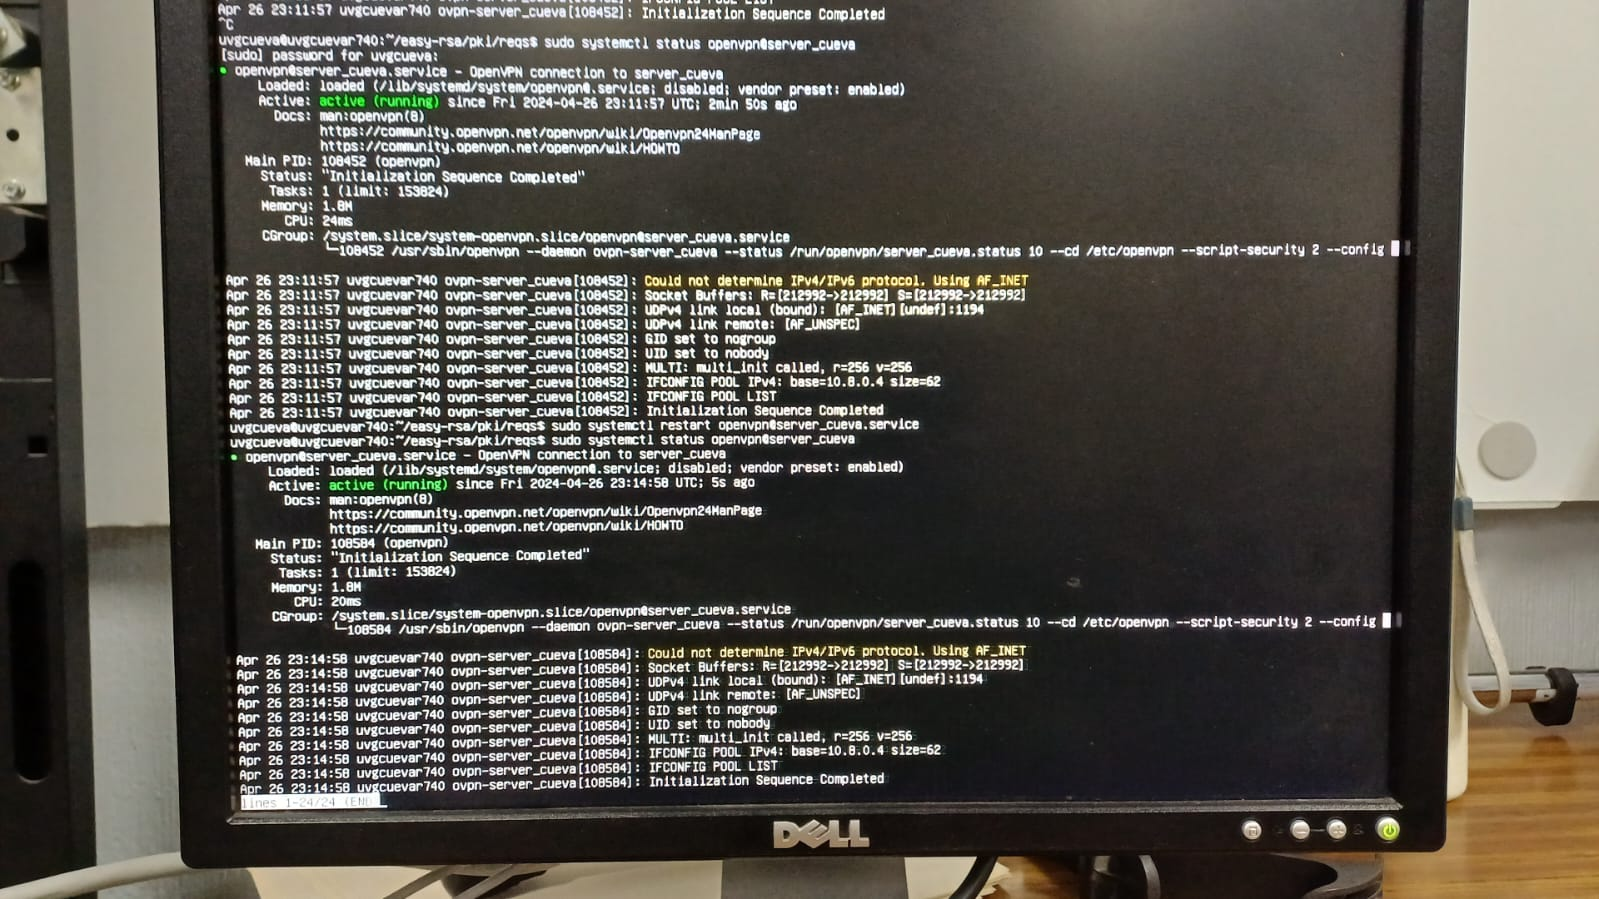
\includegraphics[width=0.7\textwidth]{figuras/LevantadoOpenVPN.png}
    \caption{LevantadoOpenVPN.}
    \label{fig:LevantadoOpenVPN}
\end{figure}
Como se puede observar en la Figura \ref{fig:LevantadoOpenVPN}, la máquina virtual ha sido levantada correctamente.

\begin{figure}[H]
    \centering
    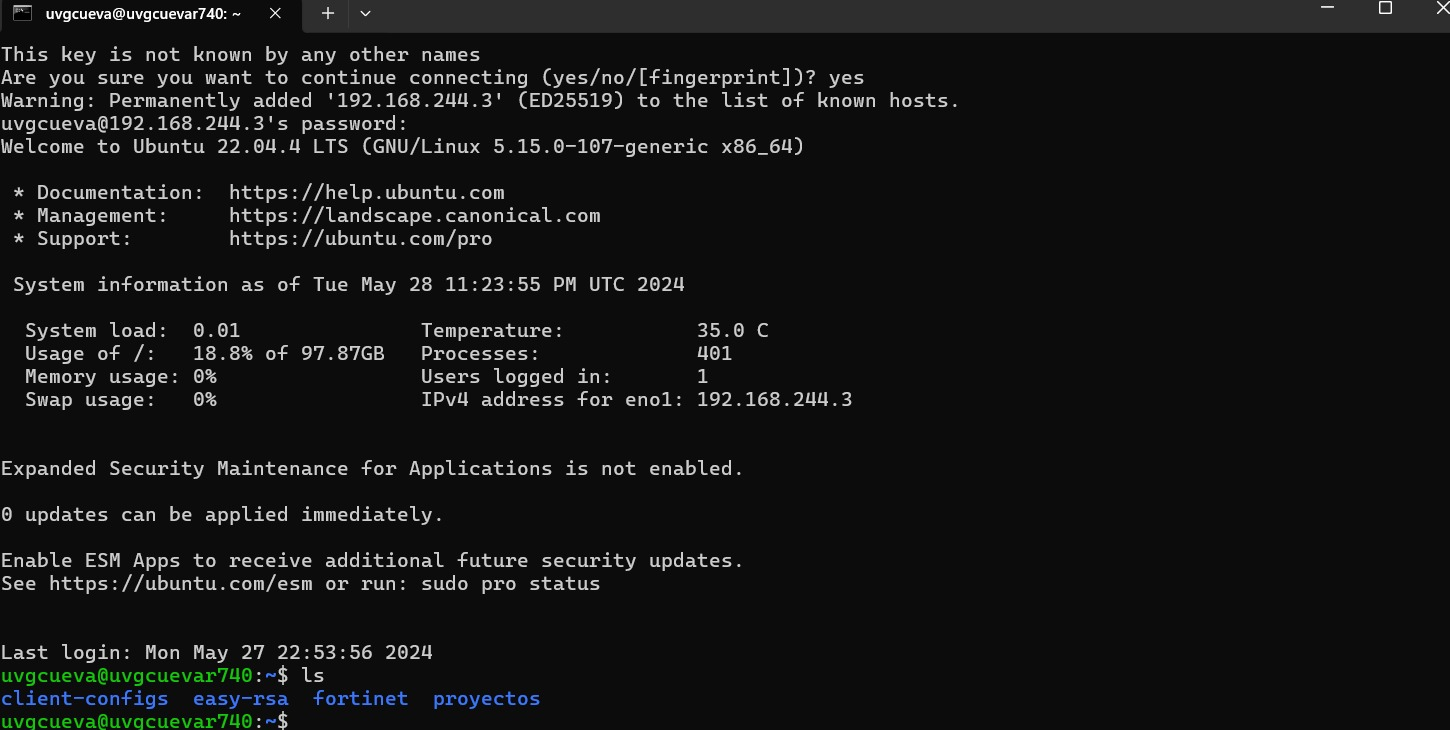
\includegraphics[width=0.7\textwidth]{figuras/ConexionSSH.png}
    \caption{ConexionSSH.}
    \label{fig:ConexionSSH}
\end{figure}
Además, en la Figura \ref{fig:ConexionSSH} se muestra la conexión generada con la VPN mediante SSH.


El proceso requiere conectarse a través de la infraestructura de red de la universidad y la VLAN específica donde se encuentra el rack y el servidor. Para lograr esto, se utiliza FortiClient VPN, que proporciona una conexión segura y cifrada directamente a la VLAN donde se encuentra el servidor. Para acceder a la VPN, se necesita un archivo de configuración .ovpn que se utiliza con OpenVPN. Una vez conectado a la VPN, se puede acceder al servidor de manera segura mediante SSH. Esto se realiza abriendo una terminal y utilizando el comando ssh uvgcueva@192.168.244.3 con las credenciales correspondientes. Este método asegura que la administración remota de las máquinas virtuales se realice de manera eficiente y segura, permitiendo a los usuarios realizar tareas administrativas y de mantenimiento sin estar físicamente presentes en el sitio.

\section{Desarrollo de la arquitectura de base de datos}

Se ha seleccionado PostgreSQL para gestionar la base de datos relacional del proyecto debido a su robustez y eficacia en el manejo de grandes volúmenes de datos, incluyendo datos de usuarios, videos y otros tipos de información. PostgreSQL ofrece avanzadas características de seguridad que son esenciales para proteger los datos contra accesos no autorizados. Su arquitectura permite realizar operaciones complejas de base de datos de manera eficiente, asegurando la integridad y la privacidad de los datos gestionados. En la arquitectura se hace especial hincapié en la importancia de diseñar con flexibilidad, utilizando estándares que permitan la interacción entre diferentes sistemas y tecnologías.

Para implementar PostgreSQL en nuestro proyecto de forma efectiva y segura, seguiremos una metodología estructurada que abarcará desde la planificación inicial hasta la integración con otros sistemas. Comenzaremos evaluando los requisitos de hardware y software para seleccionar la versión óptima de PostgreSQL y preparar el entorno del sistema operativo. Una vez instalado PostgreSQL, procederemos a configurar los parámetros de rendimiento y seguridad, como la memoria, conexiones permitidas, y configuraciones de cifrado, además de establecer un protocolo regular de mantenimiento que incluirá actualizaciones y parches.

La seguridad será una prioridad, implementando roles y permisos detallados para controlar el acceso a los datos y asegurar todas las comunicaciones mediante SSL/TLS. Paralelamente, desarrollaremos y configuraremos procesos de ETL para automatizar la extracción, transformación y carga de datos, asegurando la integridad y utilidad de la información gestionada. Además, diseñaremos y desarrollaremos APIs que permitan una interacción segura y eficiente con otras aplicaciones, implementando mecanismos robustos de autenticación y autorización.

Finalmente, estableceremos sistemas de monitoreo para supervisar constantemente el rendimiento y la seguridad de la base de datos y las APIs, permitiendo ajustes continuos para optimizar la configuración según las necesidades cambiantes del proyecto. Este enfoque metodológico asegura no solo la implementación técnica efectiva de PostgreSQL, sino también el mantenimiento de un sistema seguro, eficiente y adaptable a largo plazo.

% Cuadros de la base de datos
% ---------------------------

% Tabla: user
\begin{table}[H]
\centering
\begin{tabularx}{\textwidth}{|l|l|l|X|}
\hline
\textbf{Nombre del campo} & \textbf{Tipo de dato} & \textbf{Restricciones} & \textbf{Descripción} \\ \hline
id                       & Integer               & Primary Key            & Identificador único del usuario. \\ \hline
mail                     & String(120)           & Unique, Not Null       & Correo electrónico del usuario. \\ \hline
password                 & String(120)           & Not Null               & Contraseña del usuario. \\ \hline
streak                   & Integer               & Default = 0            & Puntuación o racha del usuario. \\ \hline
quetzalito               & String                & Nullable               & Color de la imagen de perfil. \\ \hline
confirmed                & Boolean               & Default=False          & Indica si el usuario ha confirmado su cuenta. \\ \hline
\texttt{last\_streak\_update} & DateTime            & Default=datetime.utcnow & Indica la última hora que se agregó un streak. \\ \hline
\end{tabularx}
\caption{Tabla: user}
\end{table}

% Tabla: video
\begin{table}[H]
\centering
\begin{tabularx}{\textwidth}{|l|l|l|X|}
\hline
\textbf{Nombre del campo} & \textbf{Tipo de dato} & \textbf{Restricciones} & \textbf{Descripción} \\ \hline
id                       & Integer               & Primary Key            & Identificador único del video. \\ \hline
id\_user                 & Integer               & ForeignKey(user.id), Not Null & Referencia al usuario que subió el video. \\ \hline
traduction\_esp          & String(255)           & Nullable                & Traducción del video al español. \\ \hline
sentence\_lensegua       & String(255)           & Not Null                & Oración en lengua de señas guatemalteca. \\ \hline
video                    & String(255)           & Not Null                & Ruta del archivo de video. \\ \hline
prev\_image              & String(255)           & Nullable                & Imagen previa del video. \\ \hline
is\_favorite             & Boolean               & Default=False           & Indica si el video es favorito del usuario. \\ \hline
\end{tabularx}
\caption{Tabla: video}
\end{table}

% Tabla: traducción
\begin{table}[H]
\centering
\begin{tabularx}{\textwidth}{|l|l|l|X|}
\hline
\textbf{Nombre del campo} & \textbf{Tipo de dato} & \textbf{Restricciones} & \textbf{Descripción} \\ \hline
id                       & Integer               & Primary Key            & Identificador único de la traducción. \\ \hline
id\_user                 & Integer               & ForeignKey(user.id), Not Null & Referencia al usuario que hizo la traducción. \\ \hline
sentence\_lensegua       & String(255)           & Not Null                & Oración en lengua de señas guatemalteca. \\ \hline
traduction\_esp          & String(255)           & Nullable                & Traducción al español. \\ \hline
is\_favorite             & Boolean               & Default=False           & Indica si la traducción es favorita. \\ \hline
\end{tabularx}
\caption{Tabla: traducción}
\end{table}

% Tabla: dictionary
\begin{table}[H]
\centering
\begin{tabularx}{\textwidth}{|l|l|l|X|}
\hline
\textbf{Nombre del campo} & \textbf{Tipo de dato} & \textbf{Restricciones} & \textbf{Descripción} \\ \hline
id                       & Integer               & Primary Key            & Identificador único del diccionario. \\ \hline
id\_user                 & Integer               & ForeignKey(user.id), Not Null & Referencia al usuario. \\ \hline
id\_word                 & String(255)           & Not Null                & Palabra o identificador del término en el diccionario. \\ \hline
\end{tabularx}
\caption{Tabla: dictionary}
\end{table}

El diagrama de entidad-relación presentado en la Figura \ref{fig:entidad_relacion} muestra la estructura y las relaciones entre las tablas diseñadas para el proyecto. 

En este diagrama se observan las entidades principales del sistema: \texttt{user}, \texttt{video}, \texttt{traducción} y \texttt{dictionary}. Cada una de estas entidades incluye atributos que definen su propósito dentro del sistema. Por ejemplo, la tabla \texttt{user} almacena información esencial del usuario como su correo, contraseña y estado de confirmación, mientras que la tabla \texttt{video} registra información de los videos asociados a los usuarios, incluyendo traducciones y metadatos adicionales.

Las relaciones entre las entidades destacan cómo interactúan entre sí. Por ejemplo, la tabla \texttt{video} está vinculada a la tabla \texttt{user} mediante una relación de uno a muchos (\texttt{1:N}), lo que indica que cada usuario puede tener múltiples videos asociados. Asimismo, la tabla \texttt{traducción} permite almacenar traducciones específicas realizadas por los usuarios, vinculándose también a través de una relación de \texttt{1:N} con \texttt{user}.

Este diseño garantiza la flexibilidad y escalabilidad del sistema, permitiendo el manejo eficiente de los datos necesarios para cumplir con los objetivos del proyecto.

\begin{figure}[H]
    \centering
    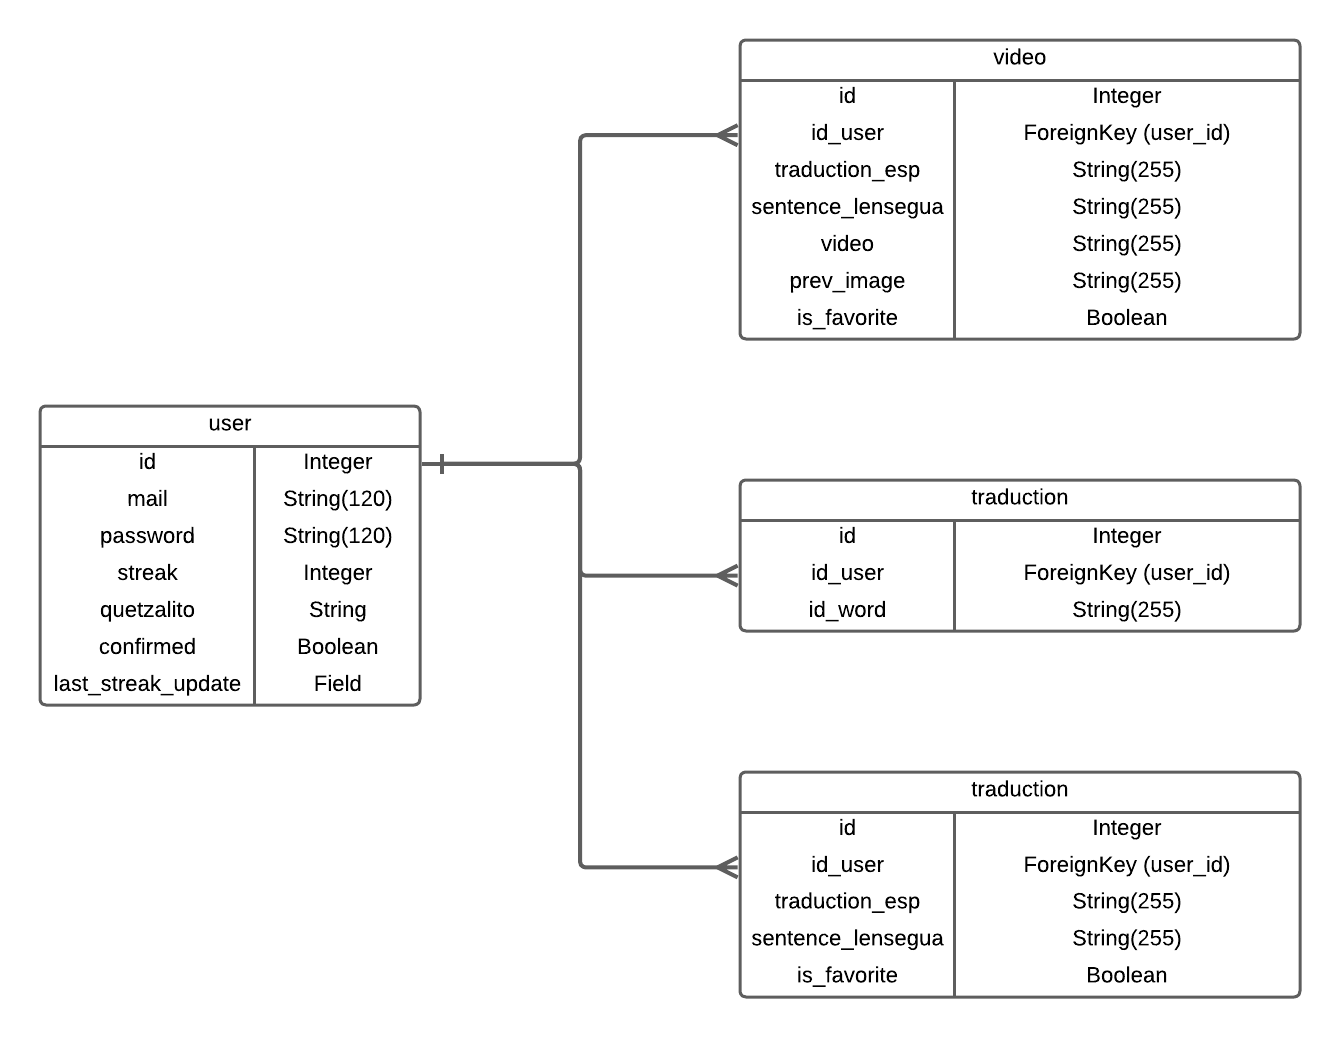
\includegraphics[width=0.5\textwidth]{figuras/entidad_relacion.png}
    \caption{Diagrama entidad relación.}
    \label{fig:entidad_relacion}
\end{figure}

% Fin de cuadros de la base de datos
% ---------------------------

\section{Implementacion de API's}

Para facilitar las consultas y las inserciones de datos, se utilizará Flask como framework principal debido a su ligereza y capacidad para manejar peticiones de manera eficiente. Este módulo API permitirá un manejo flexible de diferentes formatos de datos, incluyendo videos y texto. La estructura del módulo está diseñada para optimizar el rendimiento del sistema, minimizando el uso de recursos y maximizando la velocidad de respuesta, lo que es crucial para procesar y responder a las interacciones de los usuarios en tiempo real.

% Definir colores personalizados para las filas
\definecolor{lightgreen}{RGB}{199,233,192}
\definecolor{lightblue}{RGB}{180,220,240}
\definecolor{lightred}{RGB}{252,205,205}

% Tabla para las APIS
% -------------------

% Tabla de user_routes
\begin{table}[H]
\centering
\begin{tabularx}{\textwidth}{|l|l|l|X|}
\hline
\textbf{Nombre} & \textbf{TIPO} & \textbf{Entrada} & \textbf{Salida} \\ \hline
login & POST & email, password & id\_user \\ \hline
signup & POST & email, password, quetzalito & id\_user \\ \hline
forgot\_password & POST & email & 200-OK \\ \hline
change\_password & POST & id\_user, new\_password & id\_user, 200-OK \\ \hline
\end{tabularx}
\caption{Resumen de Rutas de API: \texttt{user\_routes}}
\label{tab:user_routes}
\end{table}

% Tabla de video_routes
\renewcommand{\arraystretch}{1.3} % Aumenta la altura de las filas
\begin{table}[H]
\centering
\begin{tabularx}{\textwidth}{|l|l|X|X|}
\hline
\textbf{Nombre} & \textbf{TIPO} & \textbf{Entrada} & \textbf{Salida} \\ \hline
send\_video & POST & id\_user, video & id\_video, traduction\_lensegua, traduction\_esp \\ \hline
report\_video & POST & id\_user, id\_video, report\_message, report\_img (png) & 200-OK \\ \hline
fav\_video & POST & id\_user, id\_video, prev\_video (png) & 200-OK \\ \hline
remove\_video & DELETE & id\_video & 200-OK \\ \hline
remove\_fav\_video & POST & id\_user, id\_video & 200-OK \\ \hline
download\_video & POST & route\_video & ruta\_video \\ \hline
download\_images & POST & route\_image & ruta\_image \\ \hline
\end{tabularx}
\caption{Resumen de Rutas de API: \texttt{video\_routes}}
\label{tab:video_routes}
\end{table}

% Tabla de traduction_routes
\begin{table}[H]
\centering
\begin{tabularx}{\textwidth}{|l|l|l|X|}
\hline
\rowcolor{blue!30} \textbf{Nombre} & \textbf{TIPO} & \textbf{Entrada} & \textbf{Salida} \\ \hline
send\_traduction & POST & id\_user, sentence\_lensegua & id\_sentence, traduction\_esp \\ \hline
fav\_traduction & POST & id\_user, id\_sentence & 200-OK \\ \hline
remove\_traduction & DELETE & id\_sentence & 200-OK \\ \hline
remove\_fav\_traduction & POST & id\_user, id\_sentence & 200-OK \\ \hline
\end{tabularx}
\caption{Resumen de Rutas de API: traduction\_routes}
\label{tab:traduction_routes}
\end{table}

% Tabla de dictionary_routes
\begin{table}[H]
\centering
\begin{tabularx}{\textwidth}{|l|l|l|X|}
\hline
\textbf{Nombre} & \textbf{TIPO} & \textbf{Entrada} & \textbf{Salida} \\ \hline
add\_dictionary & POST & id\_user, id\_word & 200-OK \\ \hline
remove\_dictionary & DELETE & id\_user, id\_word & 200-OK \\ \hline
get\_dictionary & POST & id\_user & palabras (json) \\ \hline
\end{tabularx}
\caption{Resumen de Rutas de API: \texttt{dictionary\_routes}}
\label{tab:dictionary_routes}
\end{table}

% Tabla de profile_routes
\begin{table}[H]
\centering
\begin{tabularx}{\textwidth}{|l|l|l|X|}
\hline
\textbf{Nombre} & \textbf{TIPO} & \textbf{Entrada} & \textbf{Salida} \\ \hline
get\_user\_info & POST & id\_user & email, streak, quetzalito, videos\_fav (json), traductions\_fav (json) \\ \hline
get\_video & POST & id\_user, id\_video & video (mp4) \\ \hline
get\_image & POST & id\_user, id\_video & image (png) \\ \hline
delete\_user & DELETE & id\_user & 200-OK \\ \hline
add\_streak & POST & id\_user & 200-OK \\ \hline
remove\_streak & POST & id\_user & 200-OK \\ \hline
\end{tabularx}
\caption{Resumen de Rutas de API: \texttt{profile\_routes}}
\label{tab:profile_routes}
\end{table}

% Tabla de mail_routes
\begin{table}[H]
\centering
\begin{tabularx}{\textwidth}{|l|l|l|X|}
\hline
\textbf{Nombre} & \textbf{TIPO} & \textbf{Entrada} & \textbf{Salida} \\ \hline
confirm & POST & email & 200-OK \\ \hline
\end{tabularx}
\caption{Resumen de Rutas de API: \texttt{mail\_routes}}
\label{tab:mail_routes}
\end{table}


% Fin de las tablas para APIS
% ---------------------------
% AQUI: meter la imagen de resultadosDeLlamarUsandoSQLAlchemy

\subsection{Flujo de trabajo para sistema de apis}

La infraestructura del sistema sigue un flujo bien definido en el manejo de solicitudes y respuestas, diseñado para garantizar un equilibrio entre eficiencia y robustez.

\begin{enumerate}
    \item \textbf{Cliente envía una solicitud:} 
    El punto de partida se da cuando un cliente realiza una solicitud HTTP al servidor, por ejemplo, \texttt{mi-ip:4242/example}. Este podría ser un navegador web, una aplicación móvil, o cualquier sistema que consuma las APIs que estamos desarrollando. En este primer punto, la solicitud se envía al servidor en la ruta definida.

    \item \textbf{Nginx recibe la solicitud:} 
    Nginx actúa como la primera línea de defensa y como un proxy inverso. Es el encargado de recibir todas las solicitudes entrantes y decidir cómo deben ser manejadas. Nginx no solo se encarga de redirigir las solicitudes, sino que también es clave en el manejo de conexiones concurrentes, balanceo de carga y la administración de recursos estáticos si es necesario. Gracias a Nginx, el sistema puede gestionar eficientemente un alto volumen de solicitudes simultáneas, \textit{distribuyéndolas} entre los diferentes trabajadores de Gunicorn.

    \item \textbf{Nginx reenvía la solicitud a Gunicorn:} 
    Una vez que Nginx recibe la solicitud, la reenvía a Gunicorn utilizando un socket Unix o TCP, según la configuración definida. Gunicorn es un servidor de aplicaciones WSGI diseñado específicamente para ejecutar aplicaciones Flask en entornos de producción. En este paso, Gunicorn toma la solicitud y la pasa al núcleo de la aplicación Flask.

    \item \textbf{Gunicorn procesa la solicitud:} 
    Al recibir la solicitud de Nginx, Gunicorn la envía a la aplicación Flask, encargada de manejar la lógica de negocio asociada a cada \textit{endpoint}. Por ejemplo, si la solicitud se realizó a la ruta \texttt{/example}, Flask ejecutará la función asociada a esa ruta. Esta función puede incluir lógica para consultar una base de datos, realizar cálculos, o incluso comunicarse con otros servicios.

    \item \textbf{Flask genera y envía la respuesta:} 
    Una vez que Flask ha procesado la solicitud, genera una respuesta adecuada. Esta respuesta puede estar en formato JSON, HTML, o cualquier otro formato según lo requerido por el cliente. Posteriormente, Flask devuelve la respuesta a Gunicorn, que se encargará de llevarla al siguiente paso en el flujo.

    \item \textbf{Gunicorn reenvía la respuesta a Nginx:} 
    Al recibir la respuesta de Flask, Gunicorn la reenvía a Nginx, que tiene la responsabilidad de empaquetarla y prepararla para ser entregada de vuelta al cliente.

    \item \textbf{Nginx devuelve la respuesta al cliente:} 
    Finalmente, Nginx envía la respuesta al cliente que hizo la solicitud. El cliente recibe la respuesta HTTP, que puede ser procesada y presentada de acuerdo a sus necesidades. Este paso cierra el ciclo de la solicitud, asegurando que el sistema haya gestionado de manera eficiente tanto la entrada como la salida de información.
\end{enumerate}

\subsection{Diagrama de Flujo de la Arquitectura de Solicitudes}

En esta sección se presenta el diagrama de flujo de la arquitectura del proyecto (Figura \ref{fig:diagrama_flujo}), el cual ilustra cómo se gestionan las solicitudes en el sistema. Nuestra estructura sigue el principio de "dividir y conquistar", separando las múltiples solicitudes en secciones que tienen objetivos específicos y bien definidos. 

Las solicitudes se agrupan en diferentes módulos, cada uno manejado por un archivo dedicado:
\begin{itemize}
    \item \textbf{profile\_routes.py:} Gestiona operaciones relacionadas con la información del perfil del usuario, como obtener datos personales, videos y traducciones favoritas, y la gestión de la racha (\textit{streak}).
    \item \textbf{user\_routes.py:} Maneja operaciones de autenticación y registro, como iniciar sesión, registrarse, y cambiar contraseñas.
    \item \textbf{video\_routes.py:} Se ocupa de la carga, gestión y eliminación de videos, así como de marcar o desmarcar favoritos y manejar imágenes de previsualización.
    \item \textbf{traduction\_routes.py:} Administra las traducciones de frases en Lensegua al español, permitiendo marcar traducciones como favoritas o eliminarlas.
    \item \textbf{dictionary\_routes.py:} Permite agregar, eliminar y consultar palabras en el diccionario de favoritos del usuario.
    \item \textbf{mail\_routes.py:} Facilita el envío de correos electrónicos, como en el caso de restablecimiento de contraseñas.
\end{itemize}

Todos estos módulos giran en torno al uso del archivo \textbf{models.py}, el cual actúa como el eje central del sistema. Este archivo define las entidades y modelos utilizados para interactuar con la base de datos, permitiendo que todas las secciones puedan acceder y realizar operaciones en ella de manera eficiente y centralizada.

Esta división modular asegura una arquitectura organizada, fácil de mantener y escalable, donde cada módulo se encarga de tareas específicas, mientras que el modelo central proporciona una única fuente de verdad para la interacción con los datos.

\begin{figure}[H]
    \centering
    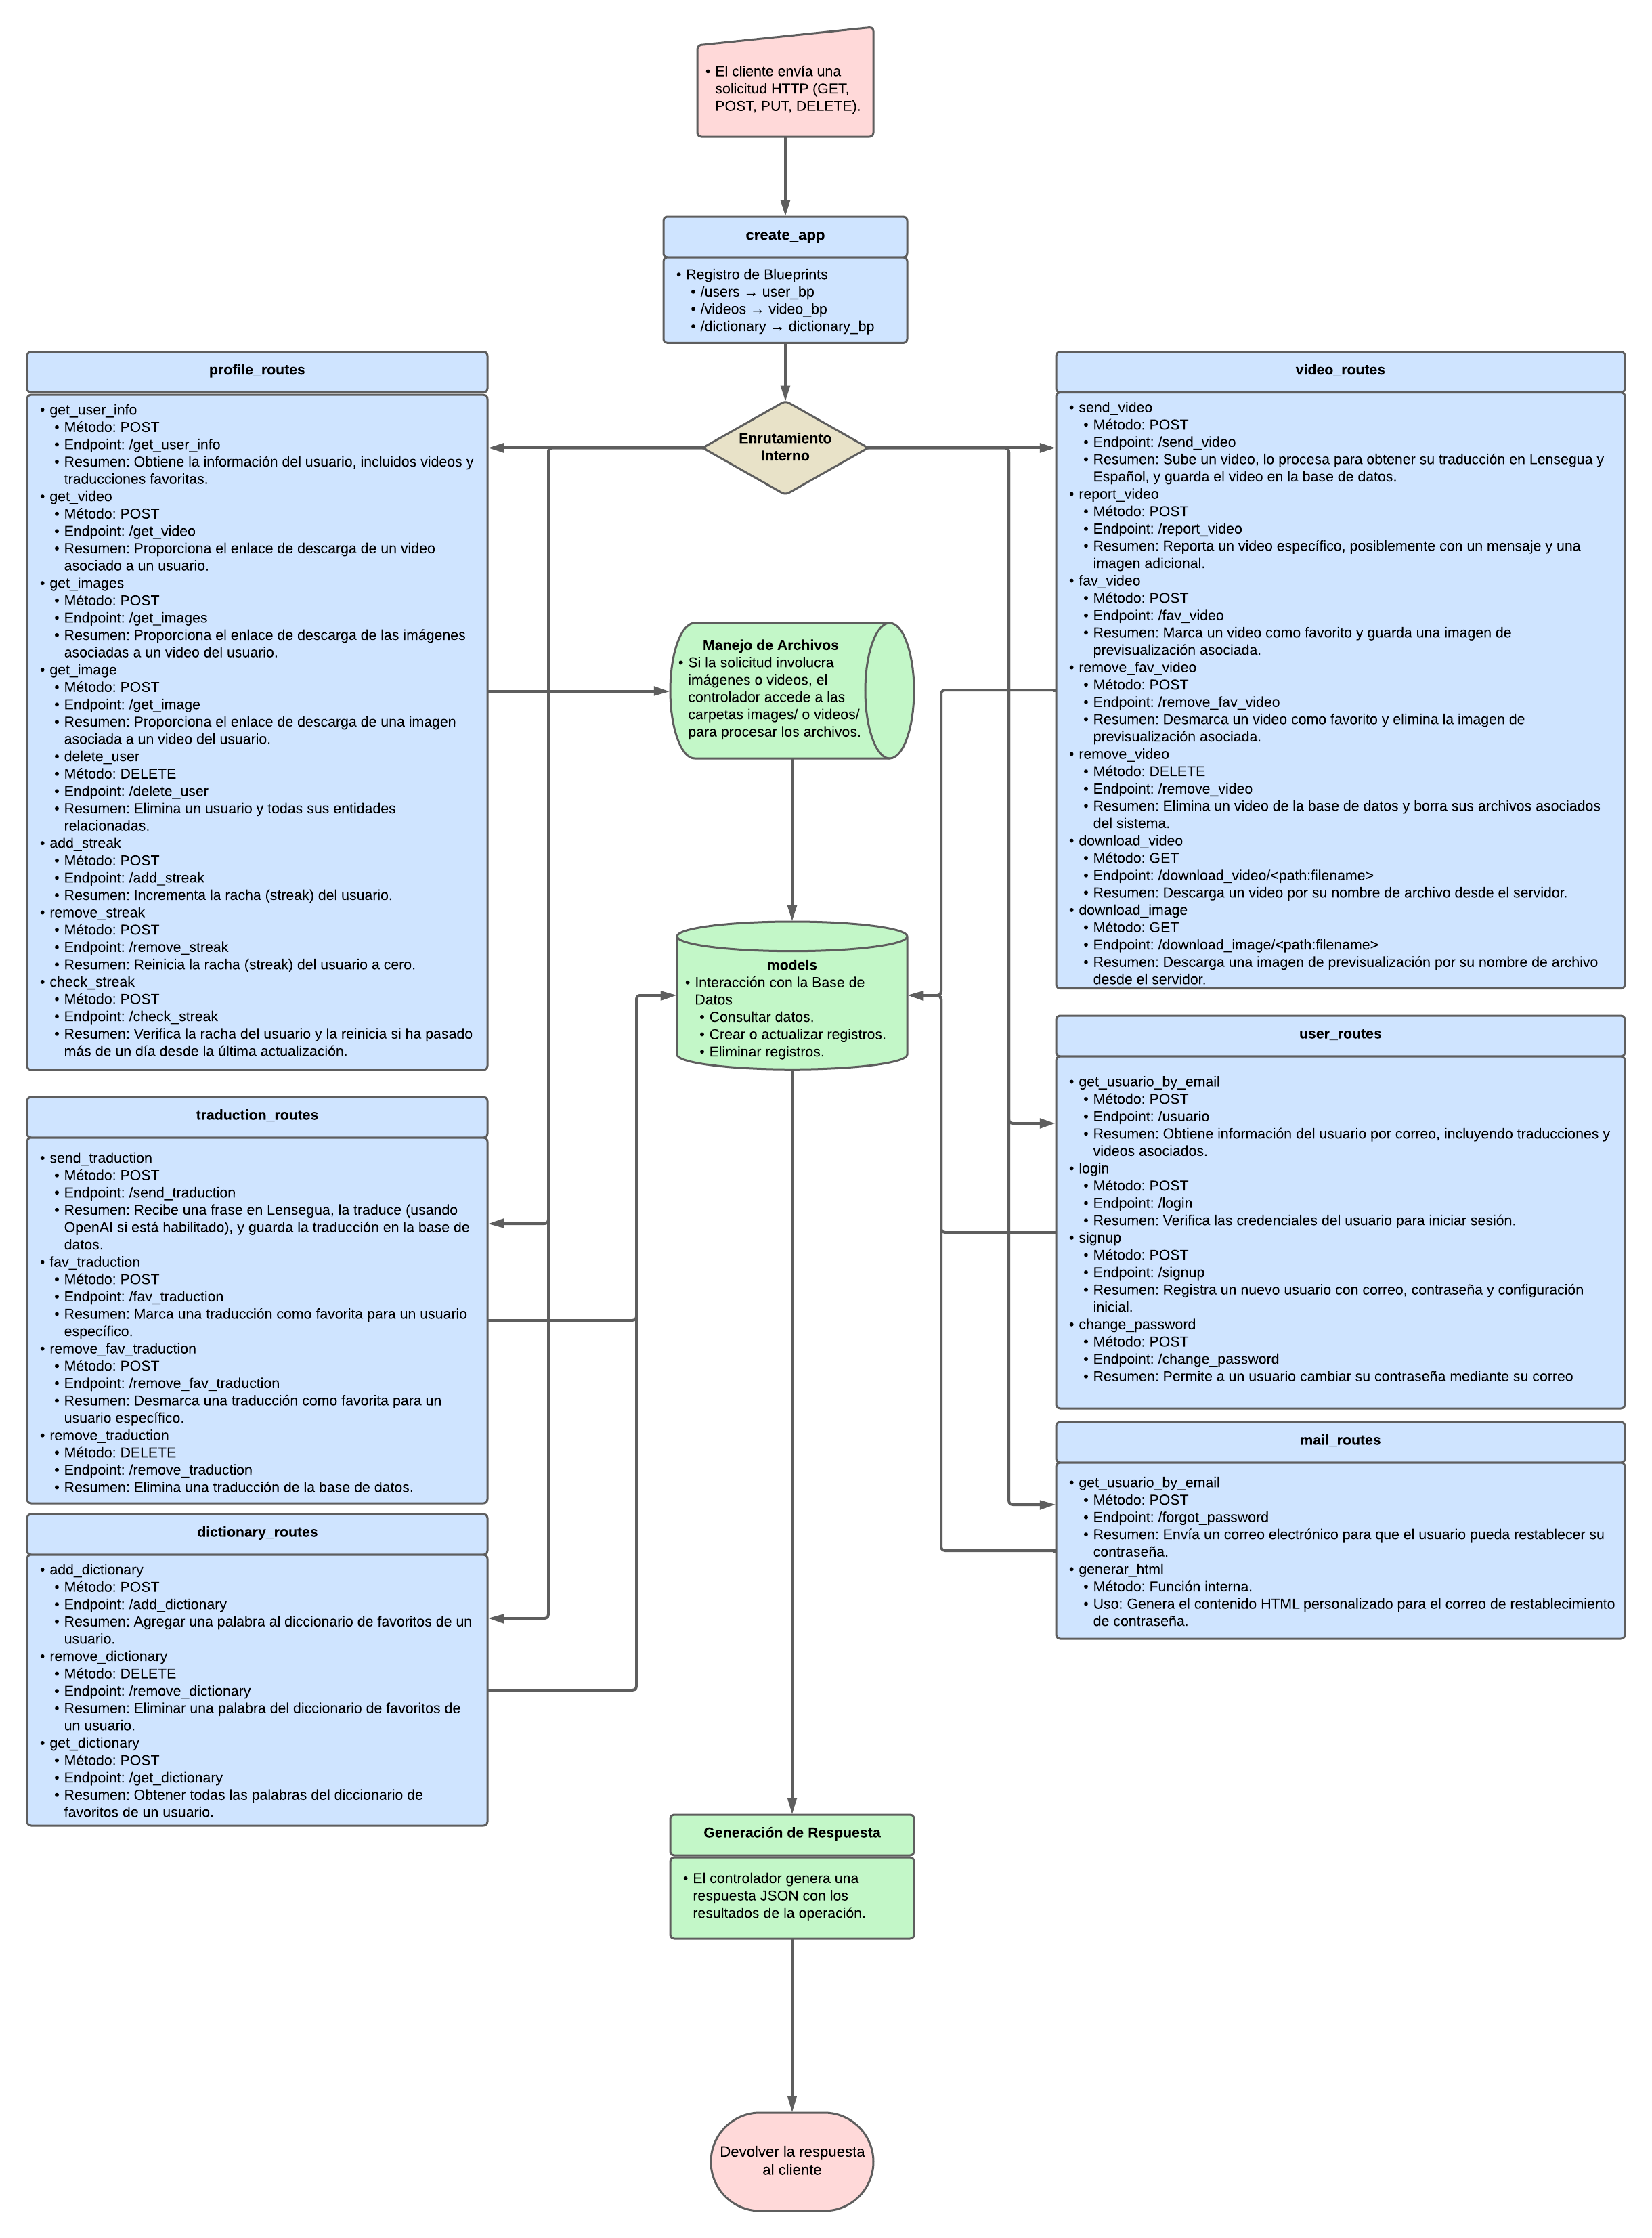
\includegraphics[width=0.5\textwidth]{figuras/diagrama_flujo.png}
    \caption{Diagrama de flujo.}
    \label{fig:diagrama_flujo}
\end{figure}

%Aqui vamos a meter lo del status y como el hacer el inicio del sistema de api-central que pues aqui se resume bien chilero y meter imagen de api-centralServiceStatus

\subsection{Implementación de Flask con GUnicorn y NGinx}

% Configuración para resaltar el código de Nginx
\lstset{
    basicstyle=\ttfamily,
    keywordstyle=\color{blue},
    frame=single,
    numbers=left,
    numberstyle=\tiny,
    breaklines=true,
    backgroundcolor=\color{gray!10}
}

% img: DiagramaImplementacionGU-NG.png
\subsection*{Componentes Principales}

\begin{enumerate}[label=\alph*)]
    \item \textbf{Flask}: Framework de Python utilizado para construir la lógica de la aplicación.
    \item \textbf{Gunicorn}: Servidor WSGI que ejecuta la aplicación Flask en un entorno de producción.
    \item \textbf{Nginx}: Proxy inverso que maneja las solicitudes del cliente, distribuye la carga, y mejora la seguridad.
\end{enumerate}

\subsection*{Flujo de trabajo del sistema de APIs:}

\begin{figure}[H]
    \centering
    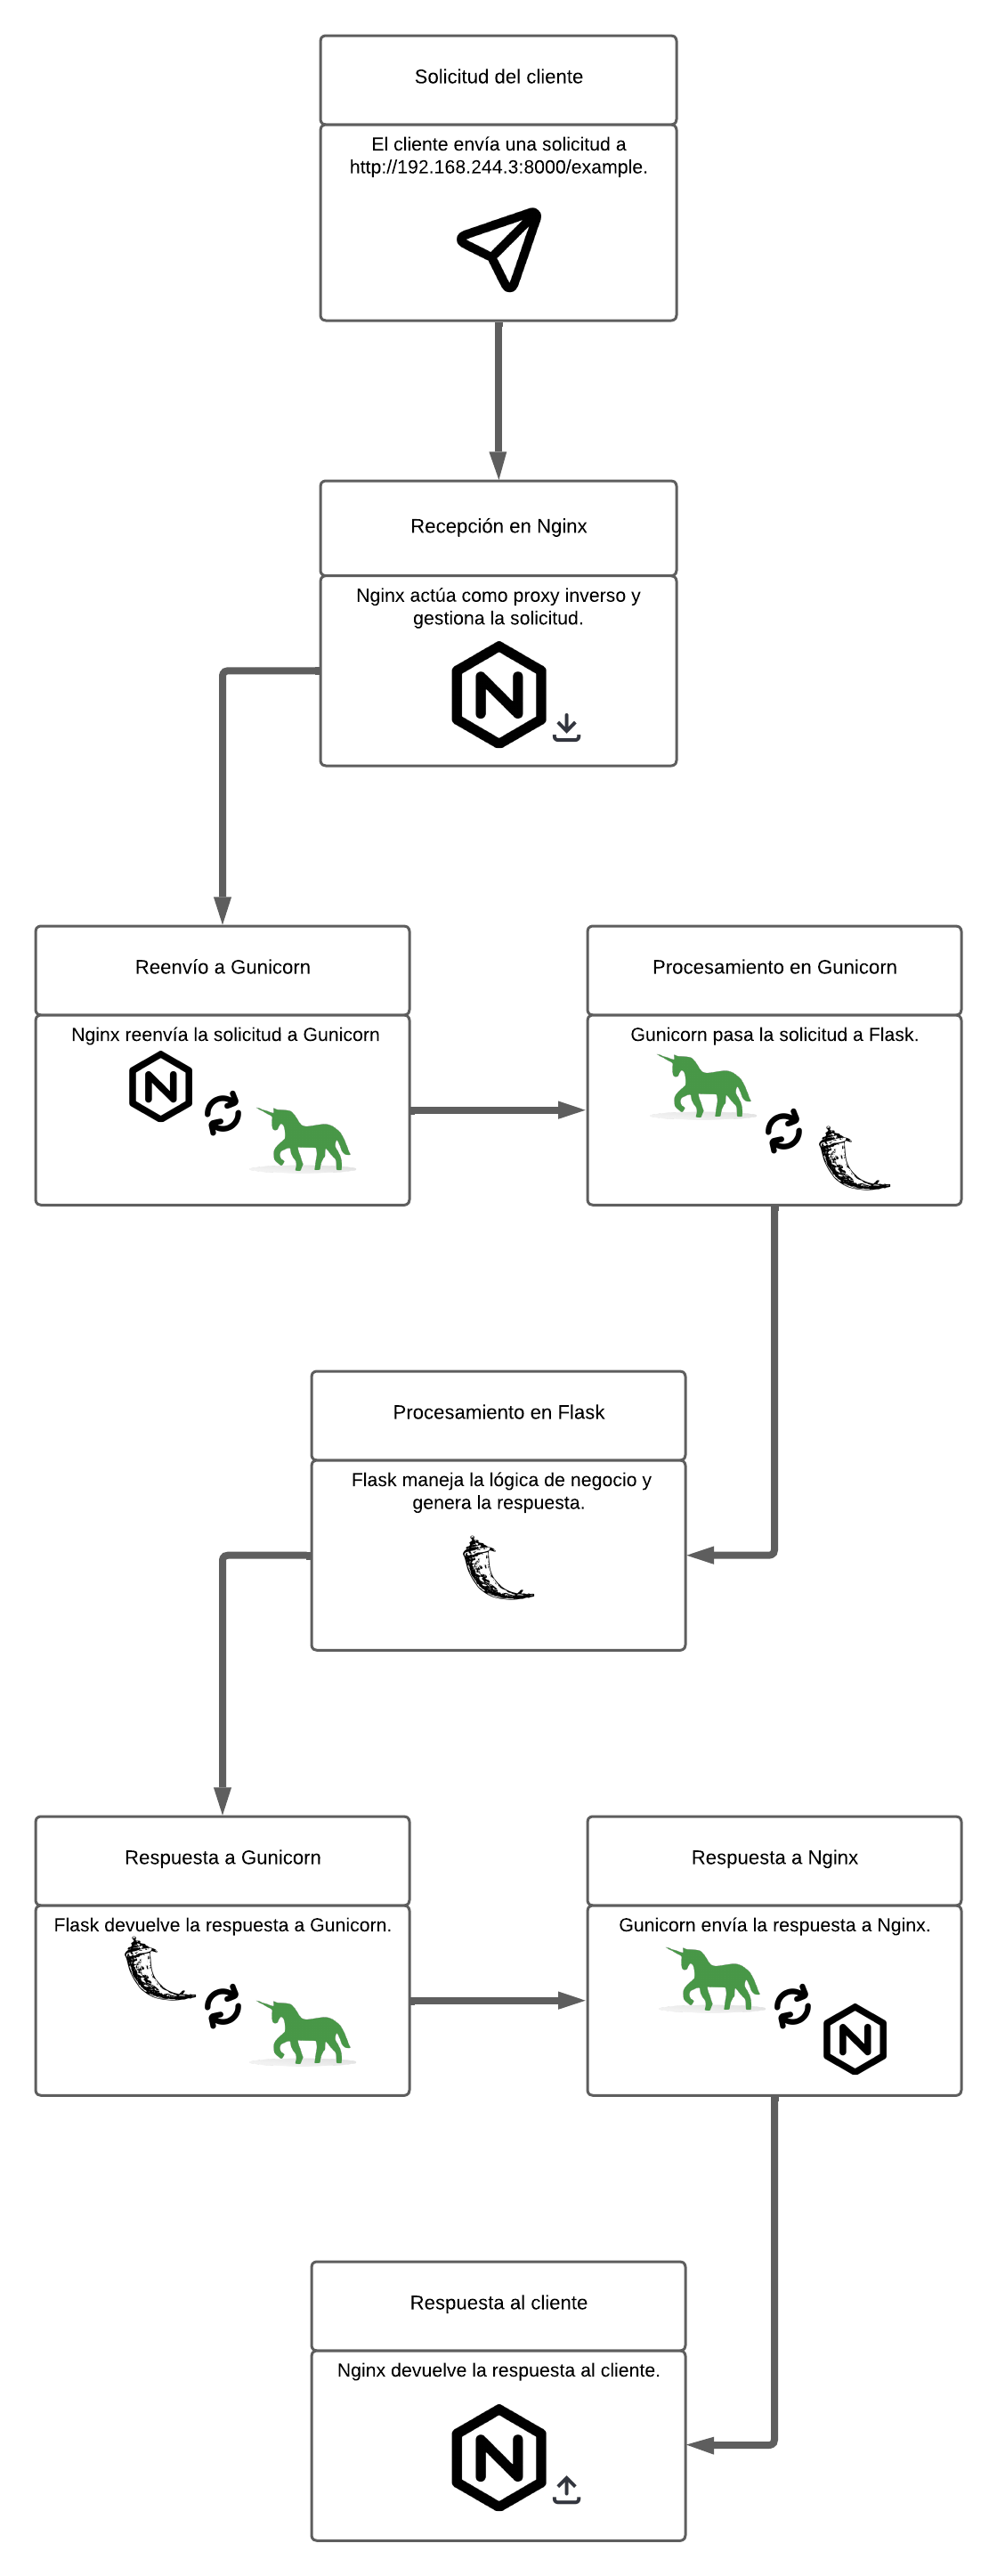
\includegraphics[width=0.5\textwidth]{figuras/DiagramaImplementacionGU-NG.png}
    \caption{Flujo de trabajo completo del sistema de APIs.}
    \label{fig:DiagramaImplementacionGU-NG}
\end{figure}

\section*{Configuración general}

\subsection*{a. Configuración de Flask}
La aplicación Flask fue configurada con soporte para migraciones de bases de datos, utilizando SQLAlchemy y Flask-Migrate. Esta configuración permite la manipulación sencilla de esquemas de bases de datos a medida que se añaden nuevas funcionalidades al sistema.

\subsection*{b. Configuración de Gunicorn}
\begin{enumerate}[label=\roman*.]
    \item Gunicorn se seleccionó como el servidor WSGI debido a su capacidad para manejar múltiples solicitudes concurrentes mediante el uso de workers. Gunicorn se ejecuta vinculándose a todas las interfaces de red en un puerto específico, lo que permite que la aplicación esté disponible en la red local o en internet.
    \item Para gestionar múltiples procesos de Gunicorn, se configuró su ejecución como un servicio del sistema. Esto asegura que Gunicorn inicie automáticamente con el sistema y facilite la gestión del servidor en producción.
\end{enumerate}

\subsection*{c. Configuración de Nginx}
\begin{enumerate}[label=\roman*.]
    \item Nginx se configuró como un proxy inverso para manejar la entrada de solicitudes del cliente y distribuirlas a Gunicorn. Este paso es crucial para manejar eficientemente la concurrencia y asegurar que el tráfico de red no sobrecargue el servidor de aplicaciones.
\end{enumerate}

\subsection*{d. Archivo de configuración de Nginx:}

\begin{lstlisting}[language=bash, caption={Archivo de configuración de Nginx.}]
server {
    listen 4242;
    server_name 192.168.244.3;

    location / {
        proxy_pass http://unix:/srv/web-apps/api-central/api-central.sock;
        include proxy_params;
        proxy_redirect off;
    }
}
\end{lstlisting}

\subsection*{Explicación del archivo de configuración de Nginx:}

\begin{enumerate}[label=\roman*.]
    \item \textbf{listen 4242}: Especifica el puerto en el que Nginx escuchará las solicitudes.
    \item \textbf{server\_name 192.168.244.3}: Define la dirección IP del servidor.
    \item \textbf{proxy\_pass}: Redirige las solicitudes recibidas a Gunicorn mediante un socket Unix, lo que mejora el rendimiento y la seguridad al evitar conexiones TCP adicionales.
    \item \textbf{include proxy\_params}: Incluye parámetros comunes para proxies inversos en Nginx.
    \item \textbf{proxy\_redirect off}: Desactiva la redirección automática de respuestas, permitiendo un control más preciso sobre el flujo de la solicitud y respuesta.
\end{enumerate}

\subsection{Implementación de SQLAlchemy para manejo de base de datos y entidades}

% AQUI: colocar imagen de migracionSqlAlchemy

\subsubsection*{1. Definición de Entidades}
Las entidades en SQLAlchemy se definen como clases que heredan de \texttt{db.Model}. Cada clase representa una tabla en la base de datos, y sus atributos corresponden a las columnas de la tabla. Por ejemplo, una entidad \texttt{Usuario} se define para representar la tabla \texttt{usuarios} con columnas como \texttt{id}, \texttt{correo} y \texttt{contrasena}. Estas clases se definen en un archivo específico, como \texttt{models.py}, para mantener el código organizado y escalable.

\subsubsection*{2. Relación entre Entidades}
SQLAlchemy permite definir relaciones entre entidades usando claves foráneas (\textit{ForeignKey}). Por ejemplo, en la entidad \texttt{Video}, existe una relación con la entidad \texttt{Usuario} mediante la columna \texttt{usuario\_id}, que referencia al \texttt{id} de la tabla \texttt{usuarios}. Este tipo de relaciones permiten manejar estructuras de datos más complejas y realizar consultas entre tablas relacionadas de forma sencilla.

\subsubsection*{3. Migraciones de Base de Datos}
Flask-Migrate se utiliza para aplicar cambios en el esquema de la base de datos de manera controlada. Una vez que las entidades están definidas, Flask-Migrate permite generar y aplicar migraciones para reflejar estos modelos en la base de datos. Este proceso se realiza en tres pasos:

\begin{enumerate}[label=\alph*.]
    \item \textbf{Inicialización de las Migraciones}: Se configura Flask-Migrate para gestionar la base de datos.
    \item \textbf{Creación de Migraciones}: Cada vez que se añade o modifica una entidad, se genera una nueva migración.
    \item \textbf{Aplicación de Migraciones}: Las migraciones se aplican a la base de datos, creando o modificando las tablas según sea necesario.
\end{enumerate}

\subsubsection*{4. Operaciones CRUD}
Con SQLAlchemy, las operaciones CRUD (Crear, Leer, Actualizar, Eliminar) se manejan fácilmente mediante el uso de sesiones de base de datos. Estas sesiones permiten realizar consultas, insertar nuevos registros, actualizar datos existentes y eliminar registros, todo de una manera declarativa y fluida.

\subsection{Implementación de módulo API para bases de datos}

Para facilitar las consultas y las inserciones de datos, se utilizará Flask como framework principal debido a su ligereza y capacidad para manejar peticiones de manera eficiente. Este módulo API permitirá un manejo flexible de diferentes formatos de datos, incluyendo videos y texto. La estructura del módulo está diseñada para optimizar el rendimiento del sistema, minimizando el uso de recursos y maximizando la velocidad de respuesta, lo que es crucial para procesar y responder a las interacciones de los usuarios en tiempo real.

% Detalle de las APIs en formato de lista
\textbf{Módulo: Procesamiento de lenguaje}
\begin{itemize}
    \item \textbf{Nombre de la API}: \texttt{API\_Procesamiento\_de\_Lenguaje}
    \item \textbf{Función de la API}: Procesar texto y generar respuestas basadas en el modelo
    \item \textbf{Entrada}: XML con texto
    \item \textbf{Salida Esperada}: Respuesta en XML del modelo GPT-4
\end{itemize}

\textbf{Módulo: Llama}
\begin{itemize}
    \item \textbf{Nombre de la API}: \texttt{API\_Llama}
    \item \textbf{Función de la API}: Analizar y responder consultas con el modelo Llama
    \item \textbf{Entrada}: XML con consulta
    \item \textbf{Salida Esperada}: Respuesta en XML del modelo Llama
\end{itemize}

\textbf{Módulo: Visión por computadora}
\begin{itemize}
    \item \textbf{Nombre de la API}: \texttt{API\_Vision}
    \item \textbf{Función de la API}: Analizar imágenes y videos, y detectar objetos
    \item \textbf{Entrada}: XML con imagen/video
    \item \textbf{Salida Esperada}: Respuesta en XML con análisis de visión por computadora
\end{itemize}

\textbf{Módulo: HyperVisor}
\begin{itemize}
    \item \textbf{Nombre de la API}: \texttt{API\_HyperVisor}
    \item \textbf{Función de la API}: Gestionar y monitorizar las máquinas virtuales
    \item \textbf{Entrada}: XML con comandos
    \item \textbf{Salida Esperada}: Respuesta en XML con estado de VMs
\end{itemize}

\subsection{API para integración de modelos de procesamiento}

Se desarrollará una API específica para facilitar la interacción entre el módulo de visión por computadora y los modelos de lenguaje natural. Esta API asegurará que la información fluya de manera eficiente desde la recepción de videos hasta la entrega de resultados en texto o voz, pasando por la consulta de bases de datos. La arquitectura de red y del servidor será diseñada para manejar altas demandas de solicitudes sin degradar la calidad del servicio, utilizando técnicas de balanceo de carga y optimización de recursos para garantizar un proceso robusto y confiable.

Se diseñará un entorno virtualizado utilizando Multipass sobre un servidor con Ubuntu 22.08 ya instalado, lo que facilitará la segregación de los módulos de visión por computadora, inteligencia artificial con GPT-4 y el modelo de IA Llama. Cada uno de estos módulos operará dentro de su propia máquina virtual, configurada específicamente para satisfacer sus requisitos operativos y de procesamiento.

Para iniciar el proceso, se configurarán máquinas virtuales individuales para cada módulo bajo el hypervisor Multipass en Ubuntu 22.08. Esta configuración implica la asignación de los recursos necesarios, como CPU dedicada, memoria RAM adecuada y espacio de almacenamiento suficiente, de acuerdo con las demandas específicas de cada aplicación. Además, se establecerán redes virtuales que permitan una comunicación eficaz y segura entre las máquinas virtuales y los sistemas de bases de datos externos.

\subsection{Implementación de Crontab}

Para garantizar que los usuarios mantengan una racha activa y que se reinicie automáticamente si ha pasado más de un día sin actividad, se ha implementado un proceso automatizado utilizando `crontab` en el servidor Linux. Esta tarea se ejecuta todos los días a las 3:00 a.m. y ejecuta un script de Python que revisa la última hora de actualización de la racha de cada usuario y la reinicia si ha pasado más de 24 horas desde la última actualización.

\subsubsection{Configuración del Cron Job}

Para configurar la tarea programada que se ejecuta a las 3:00 a.m. todos los días, se debe agregar la siguiente línea al archivo de crontab del usuario adecuado:

\lstset{
    basicstyle=\ttfamily\small,
    numbers=left,
    numberstyle=\tiny\color{gray},
    backgroundcolor=\color{lightgray!20},
    frame=single,
    captionpos=b,
    breaklines=true,
    tabsize=4,
    showstringspaces=false
}

\begin{lstlisting}[caption={Frecuencia de ejecución}, label={lst:cron_frequency}]
0 3 * * *
\end{lstlisting}
\noindent
Indica la frecuencia de ejecución (todos los días a las 3:00 a.m.).

\begin{lstlisting}[caption={Ruta al intérprete de Python}, label={lst:python_path}]
/usr/bin/python3
\end{lstlisting}
\noindent
Es la ruta al intérprete de Python.

\begin{lstlisting}[caption={Ruta al script de Python}, label={lst:script_path}]
/ruta/al/script/reset_streaks.py
\end{lstlisting}
\noindent
Es la ruta completa al script de Python que contiene la lógica de reinicio de rachas.

\begin{lstlisting}[caption={Redirección de salida y errores}, label={lst:log_redirection}]
>> /ruta/al/log/reset_streaks.log 2>&1
\end{lstlisting}
\noindent
Redirige la salida y los errores del script a un archivo de log para facilitar la revisión de su ejecución.

El script de Python que se ejecuta está diseñado para realizar las siguientes tareas:
\begin{enumerate}
    \item Crear una aplicación Flask y un contexto de aplicación para que el script pueda interactuar con la base de datos.
    \item Obtener todos los usuarios de la base de datos y revisar su última hora de actualización de racha.
    \item Calcular la diferencia de tiempo entre la hora actual y la última actualización. Si ha pasado más de 24 horas, reiniciar la racha del usuario y actualizar la hora de la última modificación.
    \item Registrar la acción en la base de datos y mostrar un mensaje de confirmación en la consola.
\end{enumerate}

\noindent
El código del script es el siguiente:

\lstset{
    language=Python,
    basicstyle=\ttfamily\small,
    numbers=left,
    numberstyle=\tiny\color{gray},
    backgroundcolor=\color{lightgray!20},
    frame=single,
    captionpos=b,
    breaklines=true,
    tabsize=4,
    showstringspaces=false
}

\begin{lstlisting}[caption={Script de restablecimiento de streaks en Flask}, label={lst:reset_streaks}]
from app import create_app, db
from app.models import User
from datetime import datetime, timedelta

# Crear la aplicación Flask y contexto
app = create_app()
app.app_context().push()

def reset_streaks():
    # Obtener todos los usuarios
    users = User.query.all()
    for usuario in users:
        if usuario.last_streak_update:
            # Calcular la diferencia de tiempo desde la última actualización
            delta = datetime.utcnow() - usuario.last_streak_update
            if delta > timedelta(days=1):
                # Ha pasado más de un día, reiniciar el streak
                usuario.streak = 0
                usuario.last_streak_update = datetime.utcnow()
                db.session.commit()
                print(f"Streak reset for user {usuario.mail}")

if __name__ == "__main__":
    reset_streaks()
\end{lstlisting}

\subsubsection{Importancia de la Implementación}

El uso de `crontab` para esta tarea es fundamental para mantener la consistencia y la precisión en el control de rachas de los usuarios sin intervención manual. Esto garantiza que las rachas de los usuarios se gestionen de manera automatizada, promoviendo un comportamiento constante y ofreciendo una mejor experiencia de usuario. Además, el uso de `crontab` permite que la tarea se ejecute en horarios de baja actividad del servidor, minimizando el impacto en el rendimiento del sistema.


\section{Virtualización del servidor para múltiples modelos}

\section*{Implementación de arquitectura con máquinas virtuales}

Para implementar esta arquitectura, se crearán un total de tres máquinas virtuales adicionales al servidor principal que actuará como HOST. Cada máquina virtual será dedicada a uno de los módulos: visión por computadora, inteligencia artificial con GPT-4 y el modelo de IA Llama.

Utilizando Multipass sobre Ubuntu 22.08, cada máquina virtual se configurará meticulosamente para cumplir con los requisitos específicos de procesamiento, asignando CPU dedicadas, memoria RAM adecuada y espacio de almacenamiento suficiente. Además, se establecerán redes virtuales para asegurar una comunicación eficiente y segura entre las máquinas virtuales y los sistemas de bases de datos. Esta configuración garantizará que cada módulo opere de manera independiente y óptima, permitiendo un procesamiento robusto y confiable bajo altas demandas de solicitudes sin comprometer la calidad del servicio.

\subsection*{Resumen del Sistema:}

\renewcommand{\arraystretch}{1.3} % Aumenta la altura de las filas
\begin{table}[H]
\centering
\begin{tabularx}{\textwidth}{|m{4cm}|m{6cm}|m{4cm}|}
\hline
\textbf{Memoria RAM} & \textbf{Espacio en disco} & \textbf{CPU} \\ \hline
Total: 125 GiB & /dev/mapper/ubuntu--vg-ubuntu--lv: 98G total, 19G usado, 75G disponible (20\% uso) & Arquitectura: x86\_64 \\ \hline
Usada: 50 MiB & /dev/sda2: 2.0G total, 253M usado, 1.6G disponible (14\% uso) & CPUs: 32 (Intel(R) Xeon(R) Silver 4216 CPU @ 2.10GHz) \\ \hline
Libre: 75 GiB & /dev/sda1: 1.1G total, 6.1M usado, 1.1G disponible (1\% uso) & Núcleos por CPU: 16 \\ \hline
Disponible: 123 GiB & & Hilos por núcleo: 2 \\ \hline
Swap Total: 8.0 GiB & & Virtualización: VT-x \\ \hline
Swap Usada: 0B & & \\ \hline
\end{tabularx}
\caption{Resumen del sistema}
\label{tab:system_summary}
\end{table}

El uso de técnicas de balanceo de carga y la optimización de recursos serán esenciales para garantizar que el sistema pueda manejar altos volúmenes de solicitudes sin comprometer la calidad del servicio. Cada máquina virtual se configurará con las dependencias y bibliotecas necesarias, garantizando que los módulos de visión por computadora y los modelos de IA operen de manera óptima y confiable dentro de este entorno virtualizado controlado.

Parte de este balanceo implica la distribución de recursos entre las máquinas virtuales. Para esto, se dividieron los recursos entre las máquinas de la siguiente manera:

\renewcommand{\arraystretch}{1.3} % Aumenta la altura de las filas
\begin{table}[H]
\centering
\begin{tabularx}{\textwidth}{|m{4.5cm}|m{4cm}|X|}
\hline
\textbf{Máquina Virtual 1 (VM1)} & \textbf{RAM: 32 GiB} & \textbf{CPUs: 8} \\ \hline
\textbf{Máquina Virtual 2 (VM2)} & \textbf{RAM: 32 GiB} & \textbf{CPUs: 8} \\ \hline
\textbf{Máquina Virtual 3 (VM3)} & \textbf{RAM: 32 GiB} & \textbf{CPUs: 8} \\ \hline
\textbf{Host (host de VM)} & \textbf{RAM: 30 GiB (restante)} & \textbf{CPUs: 8 (restante)} \\ \hline
\end{tabularx}
\caption{Distribución de recursos entre las máquinas virtuales y el host}
\label{tab:vm_resources}
\end{table}

\vspace{0.5cm}

\begin{figure}[H]
    \centering
    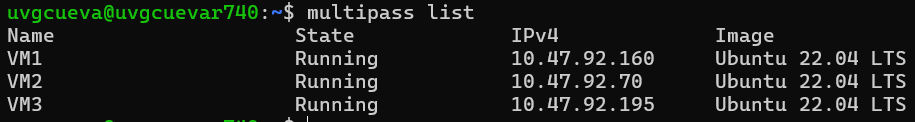
\includegraphics[width=0.5\textwidth]{figuras/EstadosVMs.png}
    \caption{Estado de las máquinas virtuales dentro del sistema}
    \label{fig:EstadosVMs}
\end{figure}

\section{Implementación de pruebas de eficiencia}

\begin{enumerate}
    \item \textbf{Instalación de Herramientas de Monitoreo:}
    \begin{enumerate}[label*=\alph*.]
        \item Instalar el agente NGINX Amplify para monitorear el uso de recursos (CPU, memoria, disco y red) en tiempo real.
        \item Adicionalmente, instalar herramientas complementarias como \texttt{htop}, \texttt{dstat}, \texttt{iotop}, \texttt{nload} y \texttt{sysdig} para monitoreo detallado y comparación de métricas.
    \end{enumerate}

    \item \textbf{Preparación del Entorno de Pruebas:}
    \begin{enumerate}[label*=\alph*.]
        \item Desarrollar un script en Python que realice solicitudes a las APIs, utilizando librerías como \texttt{requests} para solicitudes HTTP y \texttt{psutil} para monitoreo de recursos.
        \item Configurar el sistema de logging para registrar métricas en un archivo de log y enviar datos al agente NGINX Amplify.
    \end{enumerate}

    \item \textbf{Monitoreo Continuo:}
    \begin{enumerate}[label*=\alph*.]
        \item Monitorizar los recursos del sistema en tiempo real utilizando NGINX Amplify y las herramientas complementarias instaladas.
        \item Registrar métricas clave como el uso de CPU, memoria, disco y red durante las pruebas.
        \item Configurar alertas en NGINX Amplify para notificaciones automáticas sobre uso excesivo de recursos.
    \end{enumerate}

    \item \textbf{Análisis de Resultados:}
    \begin{enumerate}[label*=\alph*.]
        \item Revisar los logs generados durante las pruebas para evaluar el tiempo de respuesta y la utilización de recursos.
        \item Utilizar el panel de NGINX Amplify para analizar métricas históricas y tendencias de rendimiento.
        \item Identificar cuellos de botella y áreas de mejora mediante las métricas y gráficos proporcionados por NGINX Amplify.
    \end{enumerate}

    \item \textbf{Optimización y Repetición de Pruebas:}
    \begin{enumerate}[label*=\alph*.]
        \item Implementar ajustes necesarios en la configuración del servidor y las aplicaciones basados en los resultados del análisis.
        \item Repetir las pruebas para verificar las mejoras en el rendimiento del sistema.
        \item Continuar el ciclo de pruebas y optimización hasta alcanzar un rendimiento óptimo, utilizando NGINX Amplify para validar las mejoras.
    \end{enumerate}
\end{enumerate}

\section{Pruebas de Carga}

\subsection{Objetivo}
El objetivo de las pruebas de carga es evaluar el rendimiento del sistema bajo condiciones de carga esperadas, simulando múltiples usuarios y solicitudes concurrentes para determinar la capacidad del sistema. Estas pruebas permiten identificar posibles áreas de mejora en la infraestructura y el manejo de recursos.

\subsection{Procedimiento}
\begin{enumerate}
    \item \textbf{Simulación de Usuarios}: Se desarrolló un script en Python para crear múltiples usuarios simulados. La función \texttt{create\_users} crea registros y datos de autenticación de usuario, almacenándolos para reutilización durante la prueba.
    \item \textbf{Acciones Concurrentes}: Una vez autenticados, cada usuario simulado ejecuta una serie de acciones concurrentes usando \texttt{ThreadPoolExecutor}:
    \begin{itemize}
        \item Obtiene su información de perfil (\texttt{get\_user\_info}).
        \item Incrementa su racha de actividad (\texttt{add\_streak}).
        \item Realiza operaciones de video y traducción (subida de video, recuperación, marcación como favorito).
    \end{itemize}
    \item \textbf{Medición de Tiempos de Respuesta}: La función \texttt{send\_request} mide el tiempo de respuesta de cada operación y el estado HTTP. Esto permite registrar tiempos de respuesta y determinar si el sistema mantiene la estabilidad bajo carga.
\end{enumerate}

Para evaluar la capacidad de nuestro servidor y entender sus límites de rendimiento, realizamos una serie de pruebas de carga incrementales. Estas pruebas consistieron en simular un número creciente de usuarios concurrentes interactuando con el sistema, comenzando con 50 usuarios y aumentando progresivamente hasta 1100 usuarios. El objetivo de este enfoque es aplicar niveles crecientes de estrés en el servidor, analizando cómo responde bajo diferentes cargas de trabajo.

Cada prueba de carga permite observar el tiempo de respuesta y la estabilidad del sistema a medida que la cantidad de usuarios aumenta, identificando el punto en el que el rendimiento empieza a degradarse significativamente. Esta metodología nos ayuda a determinar la capacidad máxima de usuarios concurrentes que nuestro servidor puede manejar de forma estable antes de experimentar problemas críticos, como demoras excesivas o fallos en el procesamiento de las solicitudes. Además, este proceso de pruebas graduales nos permite identificar las métricas críticas que influencian el desempeño, tales como la utilización de CPU, la memoria disponible y el tiempo de respuesta de las solicitudes.

\newpage

%tenemos que cargar las imagenes pruebaCarga50U.png
%tenemos que cargar las imagenes pruebaCarga100U.png
%tenemos que cargar las imagenes pruebaCarga200U.png
%tenemos que cargar las imagenes pruebaCarga300U.png
%tenemos que cargar las imagenes pruebaCarga400U.png
%tenemos que cargar las imagenes pruebaCarga500U.png
%tenemos que cargar las imagenes pruebaCarga600U.png
%tenemos que cargar las imagenes pruebaCarga700U.png
%tenemos que cargar las imagenes pruebaCarga800U.png
%tenemos que cargar las imagenes pruebaCarga900U.png
%tenemos que cargar las imagenes pruebaCarga1100U.png
\begin{figure}[H]
    \centering
    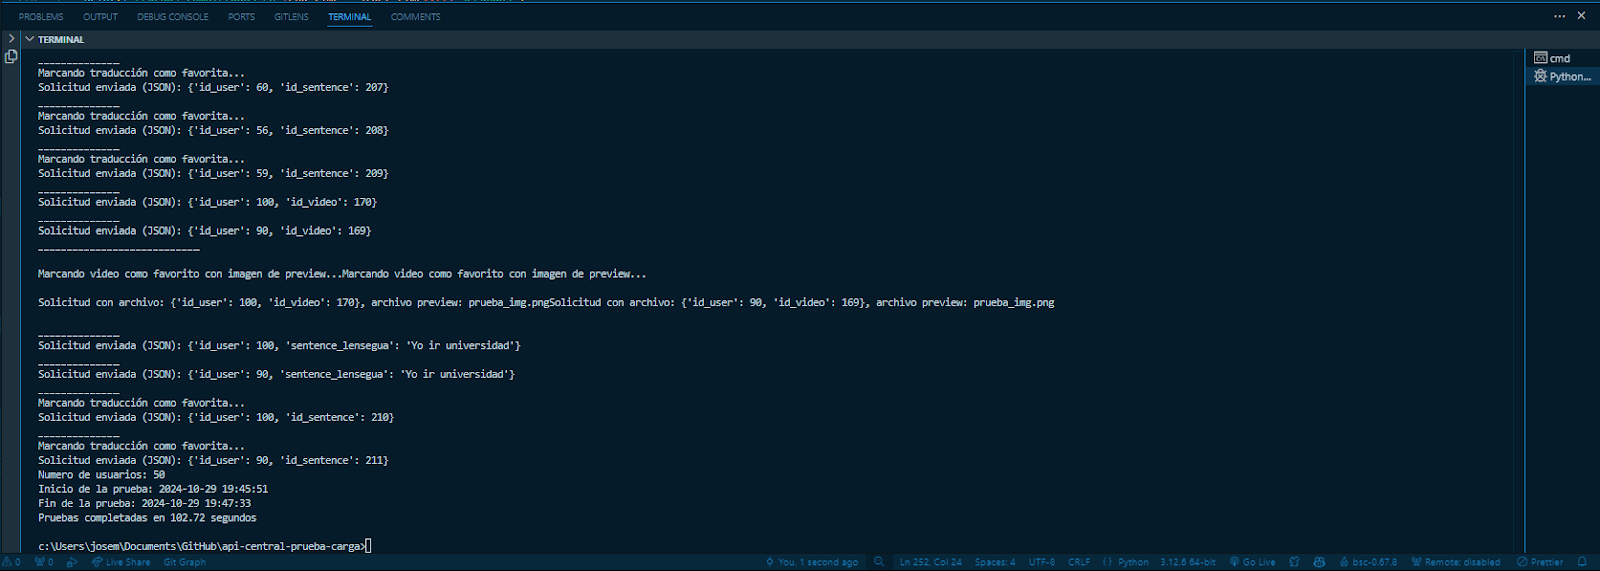
\includegraphics[width=0.5\textwidth]{figuras/pruebaCarga50U.png}
    \caption{Resultados de la prueba de carga con 50 usuarios concurrentes.}
    \label{fig:pruebaCarga50U}
\end{figure}

\begin{figure}[H]
    \centering
    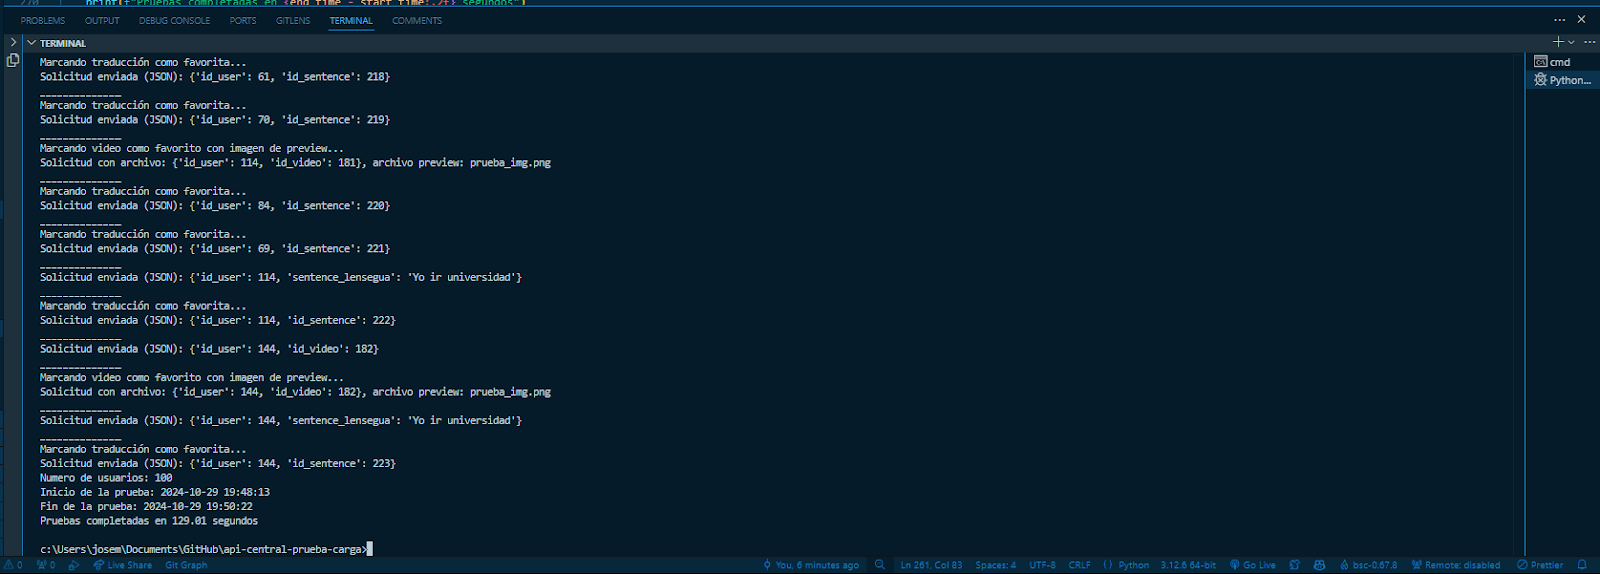
\includegraphics[width=0.5\textwidth]{figuras/pruebaCarga100U.png}
    \caption{Resultados de la prueba de carga con 100 usuarios concurrentes.}
    \label{fig:pruebaCarga100U}
\end{figure}

\begin{figure}[H]
    \centering
    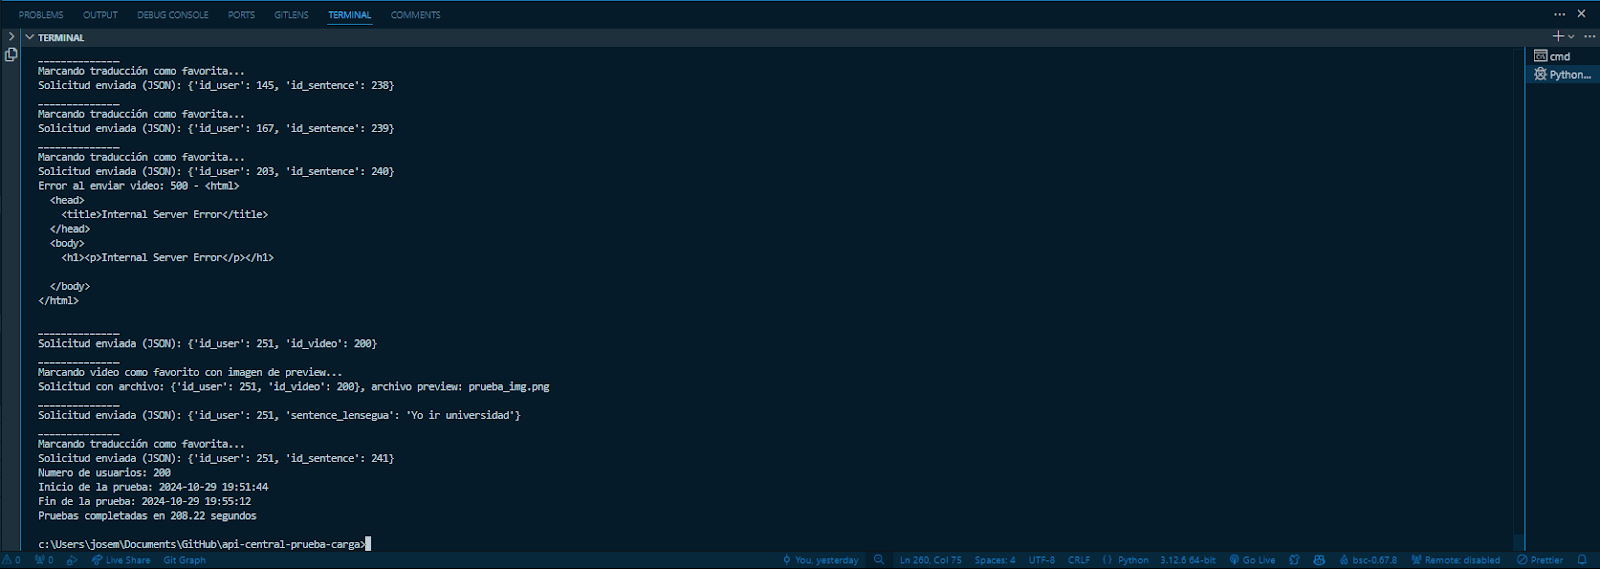
\includegraphics[width=0.5\textwidth]{figuras/pruebaCarga200U.png}
    \caption{Resultados de la prueba de carga con 200 usuarios concurrentes.}
    \label{fig:pruebaCarga200U}
\end{figure}

\begin{figure}[H]
    \centering
    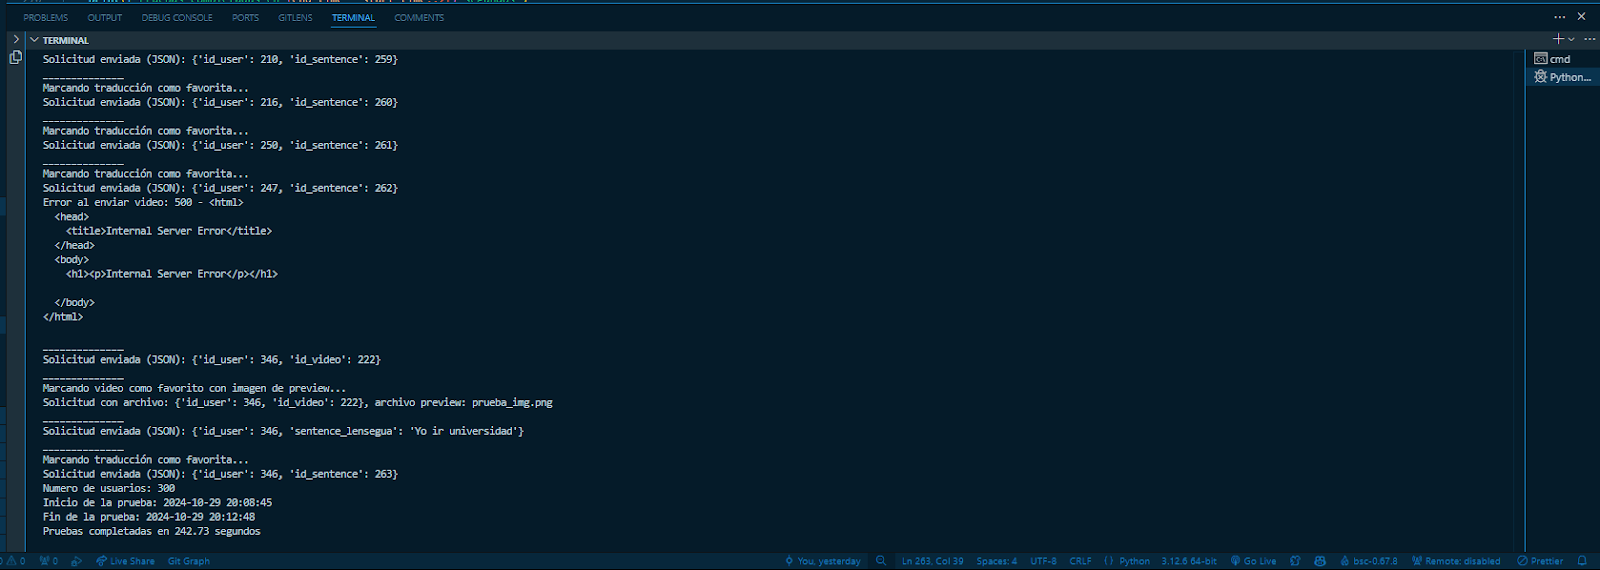
\includegraphics[width=0.5\textwidth]{figuras/pruebaCarga300U.png}
    \caption{Resultados de la prueba de carga con 300 usuarios concurrentes.}
    \label{fig:pruebaCarga300U}
\end{figure}

\begin{figure}[H]
    \centering
    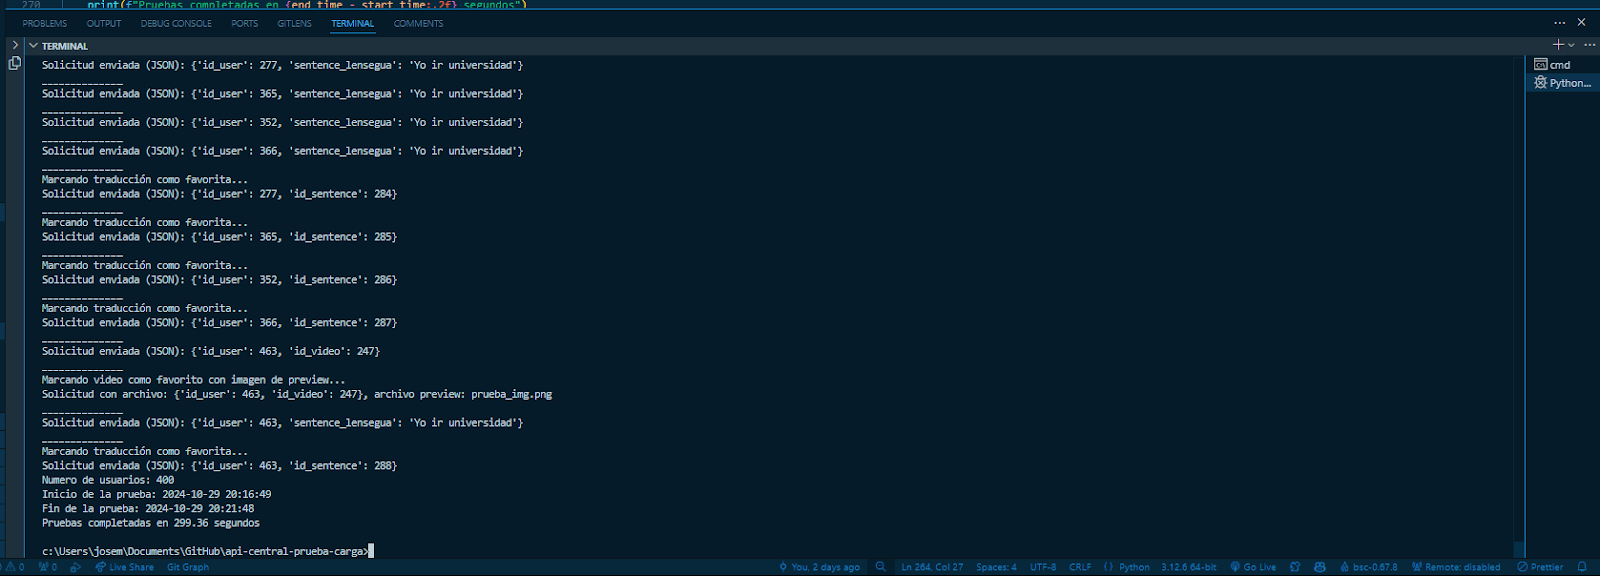
\includegraphics[width=0.5\textwidth]{figuras/pruebaCarga400U.png}
    \caption{Resultados de la prueba de carga con 400 usuarios concurrentes.}
    \label{fig:pruebaCarga400U}
\end{figure}

\begin{figure}[H]
    \centering
    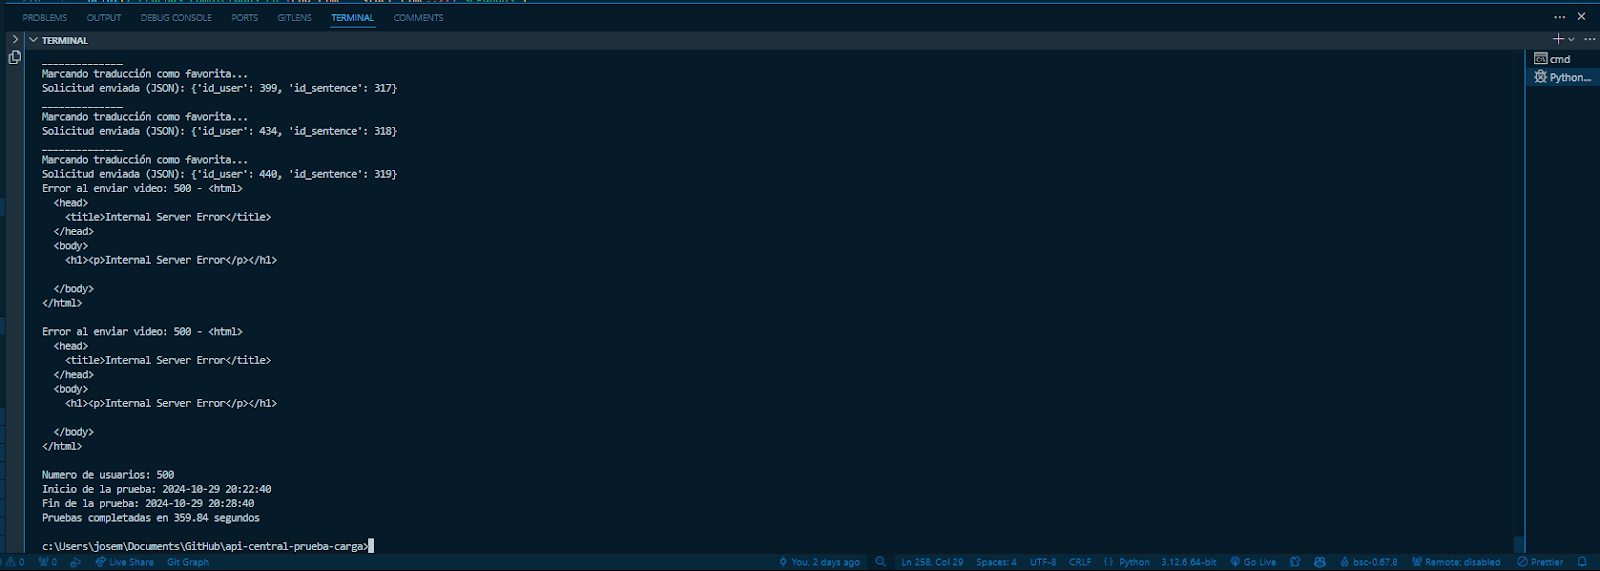
\includegraphics[width=0.5\textwidth]{figuras/pruebaCarga500U.png}
    \caption{Resultados de la prueba de carga con 500 usuarios concurrentes.}
    \label{fig:pruebaCarga500U}
\end{figure}

\begin{figure}[H]
    \centering
    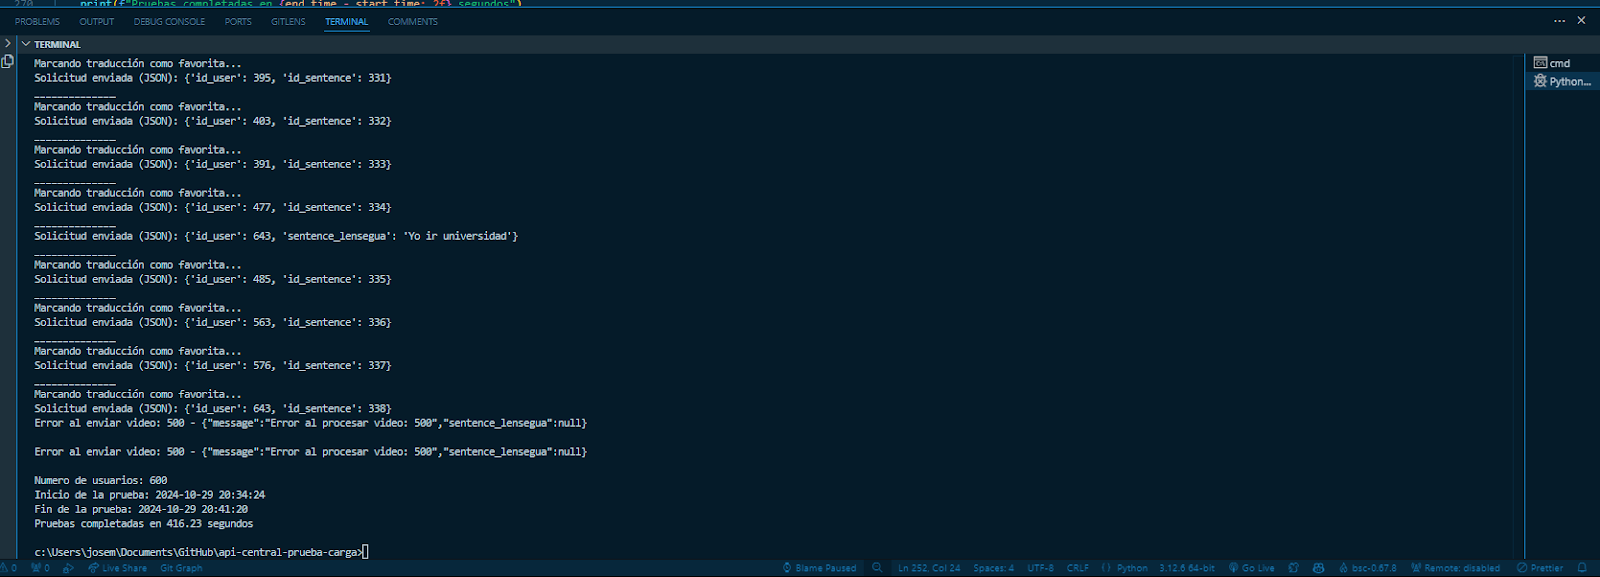
\includegraphics[width=0.5\textwidth]{figuras/pruebaCarga600U.png}
    \caption{Resultados de la prueba de carga con 600 usuarios concurrentes.}
    \label{fig:pruebaCarga600U}
\end{figure}

\begin{figure}[H]
    \centering
    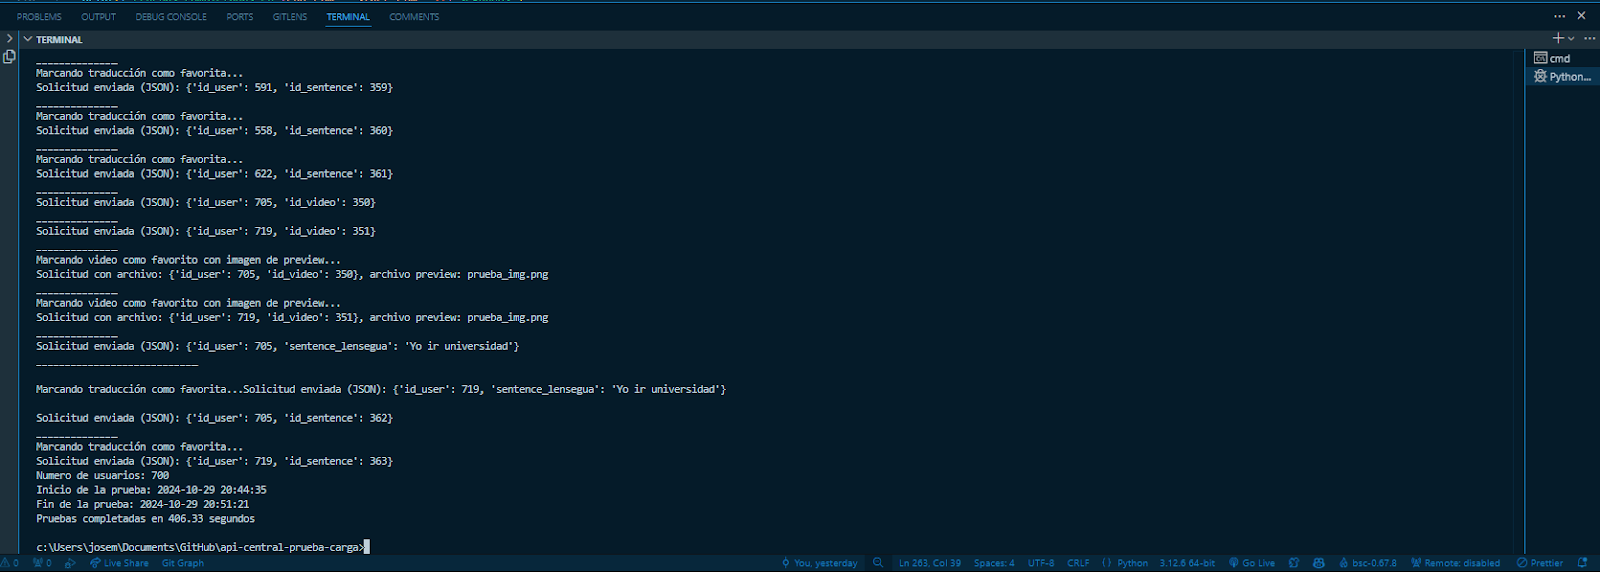
\includegraphics[width=0.5\textwidth]{figuras/pruebaCarga700U.png}
    \caption{Resultados de la prueba de carga con 700 usuarios concurrentes.}
    \label{fig:pruebaCarga700U}
\end{figure}

\begin{figure}[H]
    \centering
    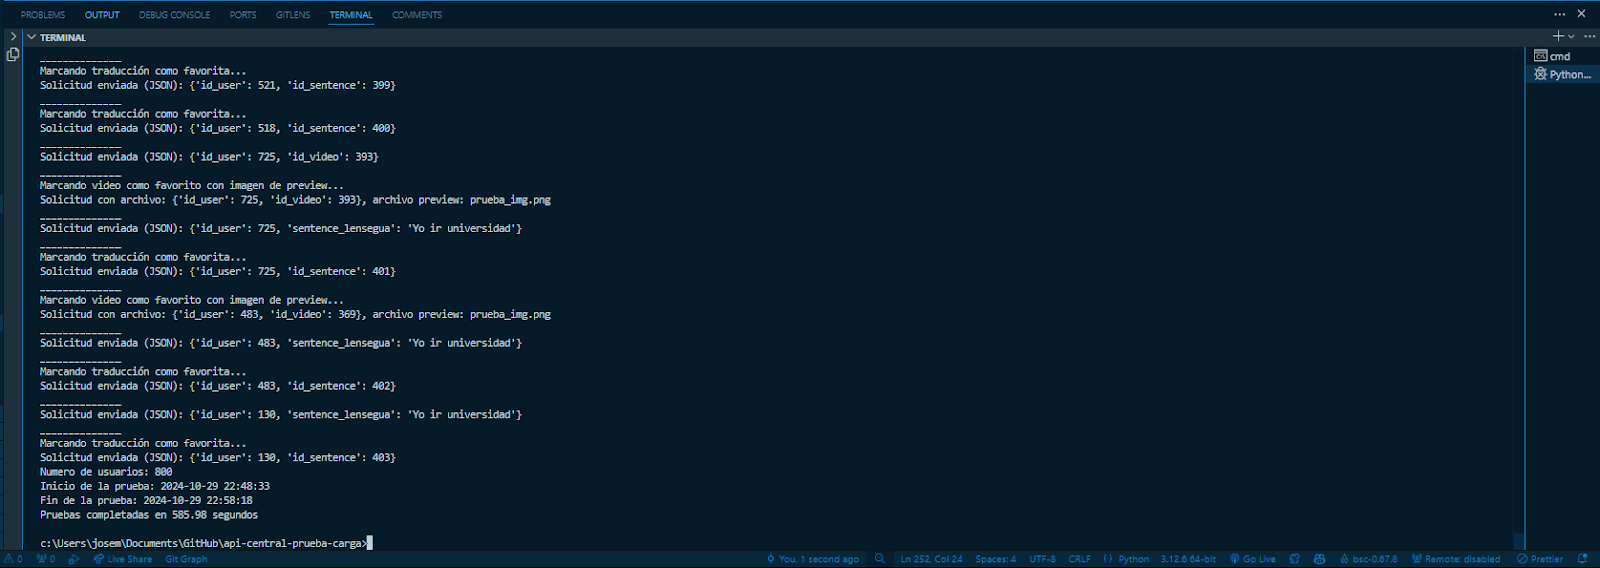
\includegraphics[width=0.5\textwidth]{figuras/pruebaCarga800U.png}
    \caption{Resultados de la prueba de carga con 800 usuarios concurrentes.}
    \label{fig:pruebaCarga800U}
\end{figure}

\begin{figure}[H]
    \centering
    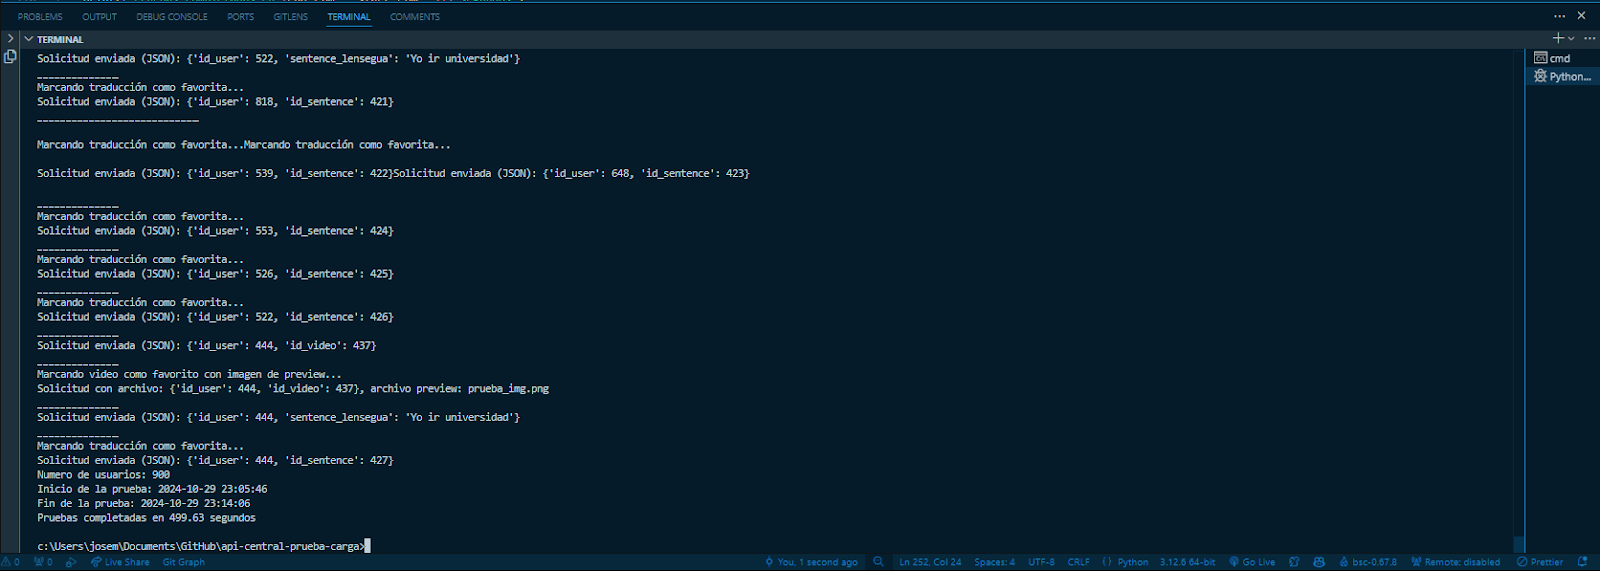
\includegraphics[width=0.5\textwidth]{figuras/pruebaCarga900U.png}
    \caption{Resultados de la prueba de carga con 900 usuarios concurrentes.}
    \label{fig:pruebaCarga900U}
\end{figure}

\begin{figure}[H]
    \centering
    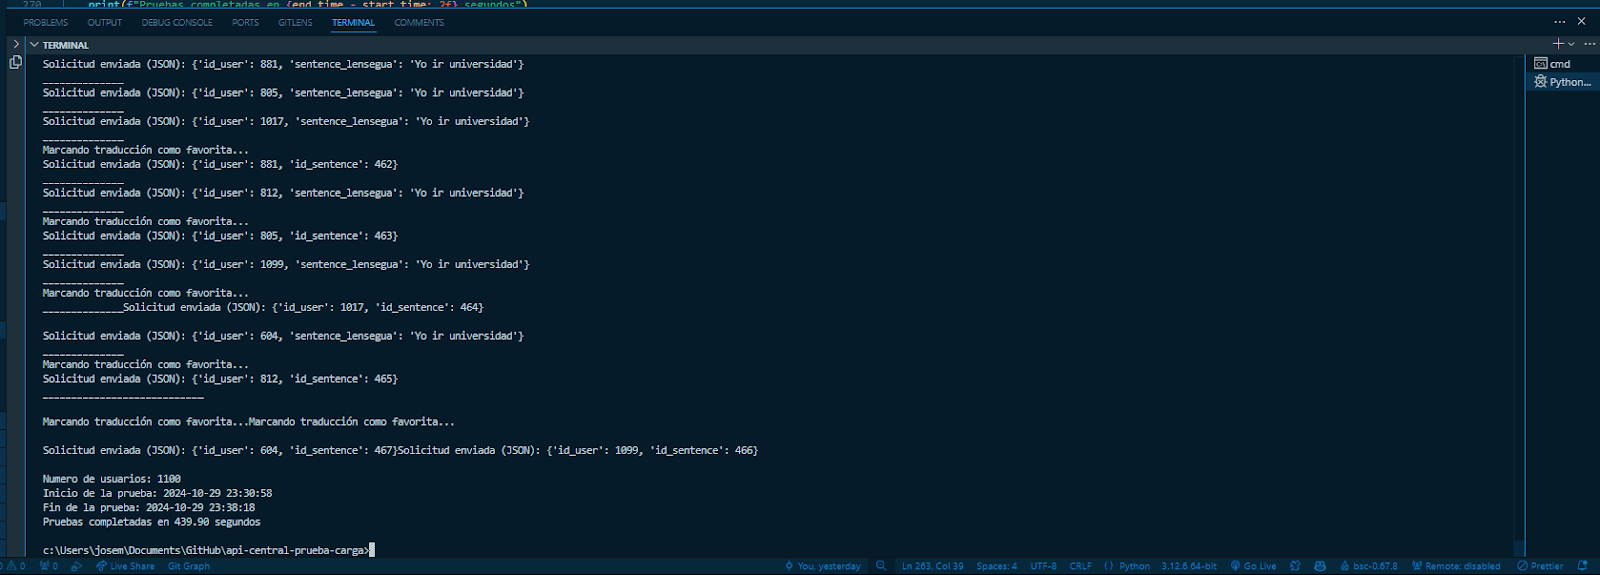
\includegraphics[width=0.5\textwidth]{figuras/pruebaCarga1100U.png}
    \caption{Resultados de la prueba de carga con 1100 usuarios concurrentes.}
    \label{fig:pruebaCarga1100U}
\end{figure}

\section{Pruebas de Extremo a Extremo (E2E)}

\subsection{Objetivo}
Las pruebas E2E validan el flujo completo de la aplicación desde la perspectiva del usuario, asegurando que todos los módulos y APIs se integren correctamente y que las funciones principales respondan adecuadamente en un flujo de uso continuo.

\subsection{Procedimiento}
\begin{enumerate}
    \item \textbf{Flujo Completo del Usuario}: Un usuario simulado realiza una serie de acciones que incluyen:
    \begin{itemize}
        \item Registro y autenticación.
        \item Acceso a su perfil, subida de video, marcación y eliminación de favoritos.
        \item Interacción con el sistema de traducciones y diccionario.
    \end{itemize}
    \item \textbf{Verificación y Tiempo de Respuesta}: Cada acción registra el tiempo de respuesta y verifica que el estado HTTP sea 200 (éxito). Esto garantiza que todas las funcionalidades respondan correctamente en un flujo integrado.
\end{enumerate}

% vamos a cargar la imagen e2e2test.png
La prueba End-to-End (E2E) se diseñó para evaluar el flujo completo de la aplicación desde la perspectiva del usuario, verificando que todas las APIs respondieran correctamente y que las funcionalidades se integraran de manera óptima. 

\section{Implementación de pruebas CVE para seguridad}

\begin{enumerate}
    \item \textbf{Identificación de Vulnerabilidades:}
    \begin{enumerate}
        \item Utilizar herramientas de escaneo de vulnerabilidades como Nessus, OpenVAS o Qualys para identificar posibles vulnerabilidades en el sistema.
        \item Asegurarse de que todas las vulnerabilidades identificadas estén referenciadas con sus respectivos identificadores CVE.
    \end{enumerate}
    
    \item \textbf{Evaluación de Vulnerabilidades:}
    \begin{enumerate}
        \item Realizar pruebas exhaustivas de seguridad para obtener los datos necesarios para la calculadora CVSS. Las pruebas incluyen:
        \begin{enumerate}
            \item Pruebas de Explotabilidad: Evaluar cuán fácilmente se puede explotar la vulnerabilidad, incluyendo factores como la complejidad del ataque y los privilegios requeridos.
            \item Pruebas de Impacto: Medir el impacto potencial de la vulnerabilidad en la confidencialidad, integridad y disponibilidad del sistema.
            \item Pruebas de Alcance: Determinar si la vulnerabilidad afecta sólo al componente vulnerable o si se puede propagar a otros componentes.
        \end{enumerate}
        \item Recopilar los datos obtenidos de las pruebas y utilizar una calculadora de puntaje CVE, como la proporcionada por el NVD (National Vulnerability Database), para calcular el puntaje de cada vulnerabilidad basada en los criterios de CVSS (Common Vulnerability Scoring System).
        \item \textbf{Criterios de CVSS:}
        \begin{enumerate}
            \item \textbf{Base Score}: Evaluación del impacto y la facilidad de explotación de la vulnerabilidad.
            \item \textbf{Temporal Score}: Considera factores temporales como la disponibilidad de explotaciones y parches.
            \item \textbf{Environmental Score}: Ajusta el puntaje base según el entorno y la configuración específicos.
        \end{enumerate}
    \end{enumerate}

    \item \textbf{Validación de Medidas de Seguridad:}
    \begin{enumerate}
        \item Implementar y validar las medidas de mitigación necesarias para corregir las vulnerabilidades identificadas.
        \item Realizar pruebas de validación post-mitigación para asegurar que las vulnerabilidades hayan sido corregidas y que las medidas no afecten negativamente el rendimiento del sistema.
    \end{enumerate}

    \item \textbf{Monitoreo Continuo:}
    \begin{enumerate}
        \item Realizar escaneos periódicos de vulnerabilidades para identificar nuevas amenazas y asegurarse de que las vulnerabilidades conocidas estén mitigadas.
        \item Recalcular los puntajes de CVE periódicamente para asegurar que el sistema se mantenga seguro.
    \end{enumerate}

    \item \textbf{Documentación y Reportes:}
    \begin{enumerate}
        \item Mantener un registro detallado de todas las vulnerabilidades identificadas, sus puntajes CVE y las acciones de mitigación realizadas.
        \item Generar reportes periódicos que incluyan análisis de tendencias en las vulnerabilidades y la efectividad de las medidas de seguridad implementadas.
    \end{enumerate}

    \item \textbf{Optimización y Mejora Continua:}
    \begin{enumerate}
        \item Basado en los análisis de vulnerabilidades y puntajes CVE, implementar ajustes necesarios en la configuración del servidor y las aplicaciones.
        \item Repetir las pruebas de seguridad para verificar las mejoras en la protección del sistema.
        \item Continuar el ciclo de pruebas y optimización hasta alcanzar un nivel óptimo de seguridad.
    \end{enumerate}
\end{enumerate}

\section{Pruebas de Seguridad con Lynis}

\subsection{Objetivo}
En este proyecto, se utilizó Lynis para auditar la seguridad del sistema mediante su Índice de Fortalecimiento. Este índice proporcionó una evaluación cuantitativa basada en la implementación de medidas de seguridad y prácticas recomendadas. Para cumplir con los objetivos del sistema, se definió una meta inicial de un puntaje de 40, considerado como la base para garantizar un sistema con medidas de seguridad básicas adecuadas. Este enfoque siguió las recomendaciones de la documentación de Lynis Hardening Index \cite{LynisHardeningIndex}, que establecía que un puntaje de 40 era suficiente para aplicaciones estándar, mientras que resultados más altos reflejaban un sistema más robusto. Según el CIS Benchmark \cite{CISBenchmarksReport}, una auditoría con un puntaje superior a 50 indicaba un fortalecimiento razonable para sistemas en entornos no críticos.

\subsection{Procedimiento}
\begin{enumerate}
    \item \textbf{Instalación y Ejecución}: Lynis fue instalado y ejecutado con el siguiente comando:
    \begin{verbatim}
    sudo lynis audit system
    \end{verbatim}
    Al finalizar, Lynis generó un informe con recomendaciones específicas para mejorar la seguridad del sistema.
    
    \item \textbf{Interpretación del Informe}: El informe proporcionado incluyó una puntuación general de seguridad, destacando las áreas de mayor riesgo y ofreciendo recomendaciones detalladas. 
\end{enumerate}

\section{Mejoras de Seguridad en \texttt{/etc/sysctl.conf}}

En base a las recomendaciones de Lynis, se realizaron ajustes en el archivo \texttt{/etc/sysctl.conf} para mejorar la seguridad de red del sistema. Estas configuraciones incluyen:

\begin{itemize}
    \item \textbf{Deshabilitar redirecciones ICMP} para prevenir ataques de red.
    \item \textbf{Habilitar SYN Cookies} para mitigar ataques SYN flood.
    \item \textbf{Restringir el uso de \texttt{dmesg} para usuarios no privilegiados}.
\end{itemize}

\section{Monitoreo Continuo de Seguridad con ClamAV}

\subsection{Instalación y Configuración}
ClamAV y su servicio de actualización \textbf{freshclam} fueron instalados para realizar escaneos de seguridad en el sistema de manera regular. Esto garantiza una capa adicional de protección contra amenazas de malware.

\subsection{Monitoreo y Ajustes Adicionales}
El sistema fue configurado para realizar escaneos periódicos y actualizar la base de datos de ClamAV. Esto permite mantener el sistema protegido frente a vulnerabilidades potenciales en el software o archivos nuevos.

\fi

% Resultados
% --------------------------------------------------------------------------------

\newpage
\thispagestyle{empty}
\mbox{}
\newpage 

\ifdefined\CAPresultados
	\newpage
	\chapter{Resultados}
	\ifdefined\parpordefecto
		\defaultparformat{resultados}
	\else
		\section{Redireccionamiento de puertos para acceso SSH Externo}

Una vez asignados los recursos, se procede a la configuración de la red y acceso remoto para cada máquina virtual. Mediante la implementación de reglas de redireccionamiento de puertos \textbf{con iptables}, se permite el acceso a las VMs desde el exterior a través de SSH. Cada máquina virtual se ha configurado para ser accesible mediante un puerto específico: \textbf{2222 para VM1}, \textbf{2223 para VM2} y \textbf{2224 para VM3}. Este esquema de puertos permite una administración centralizada y segura desde cualquier ubicación externa, sin necesidad de modificar la configuración interna de las VMs.

\begin{itemize}
    \item \textbf{Para VM1 (puerto 2222)}
    \begin{itemize}
        \item \texttt{sudo iptables -t nat -A PREROUTING -p tcp --dport 2222 -j \newline
        DNAT --to-destination 10.47.92.160:22}
        
        \item \texttt{sudo iptables -t nat -A POSTROUTING -p tcp -d 10.47.92.160 \newline
        --dport 22 -j MASQUERADE}
    \end{itemize}
    
    \item \textbf{Para VM2 (puerto 2223)}
    \begin{itemize}
        \item \texttt{sudo iptables -t nat -A PREROUTING -p tcp --dport 2223 -j \newline
        DNAT --to-destination 10.47.92.70:22}
        
        \item \texttt{sudo iptables -t nat -A POSTROUTING -p tcp -d 10.47.92.70 \newline
        --dport 22 -j MASQUERADE}
    \end{itemize}
    
    \item \textbf{Para VM3 (puerto 2224)}
    \begin{itemize}
        \item \texttt{sudo iptables -t nat -A PREROUTING -p tcp --dport 2224 -j \newline
        DNAT --to-destination 10.47.92.195:22}
        
        \item \texttt{sudo iptables -t nat -A POSTROUTING -p tcp -d 10.47.92.195 \newline
        --dport 22 -j MASQUERADE}
    \end{itemize}
\end{itemize}


Estas reglas fueron guardadas y aplicadas de manera persistente para asegurar su disponibilidad tras cualquier reinicio. El acceso SSH se configuró adicionalmente para utilizar claves públicas generadas desde sistemas Windows, facilitando una autenticación segura y sin contraseña.

En cuanto a la seguridad de las bases de datos, se decidió utilizar MySQL Server, gestionando la contraseña del usuario root para fortalecer la protección. El comando \texttt{ALTER USER} fue utilizado para actualizar la contraseña y asegurar que el acceso sea exclusivo desde el host local, minimizando riesgos.

Esta metodología garantiza una infraestructura virtualizada sólida, segura y eficiente, diseñada para soportar altas demandas y mantener la estabilidad bajo cargas intensivas.

\section{Resultados de la Prueba de Carga}

Para evaluar el rendimiento del servidor, se realizaron pruebas de carga con un número creciente de usuarios concurrentes. A continuación, se presentan los resultados obtenidos y las métricas de rendimiento observadas.

\begin{figure}[H]
    \centering
    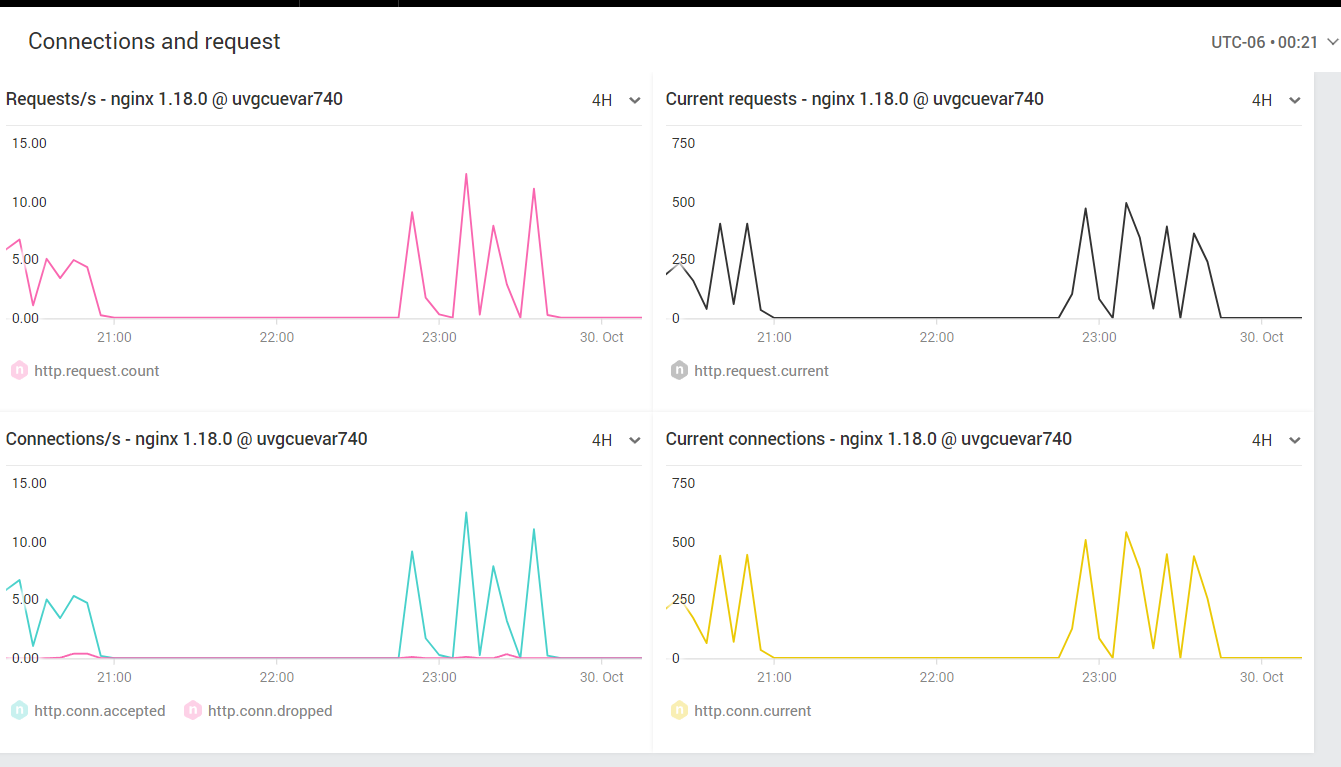
\includegraphics[width=0.8\textwidth]{figuras/ConnectionsAndRequest.png}
    \caption{Métricas de Conexiones y Solicitudes: Requests/s y Conexiones Actuales}
    \label{fig:connectionsAndRequest}
\end{figure}

\paragraph{Requests/s y Conexiones Actuales}
El servidor mostró un buen manejo de solicitudes por segundo (requests/s), manteniendo una cantidad de peticiones estable hasta las pruebas con una carga elevada. Esto demuestra que la configuración de NGINX y Gunicorn está bien ajustada para recibir y gestionar una alta cantidad de solicitudes concurrentes. Los picos de conexiones actuales también son gestionados adecuadamente, lo que indica que NGINX puede aceptar múltiples conexiones sin saturarse. La configuración con Gunicorn, que permite manejar conexiones asincrónicas y de múltiples hilos, ayuda a procesar solicitudes de manera eficiente y a mantener baja la latencia.

\begin{figure}[H]
    \centering
    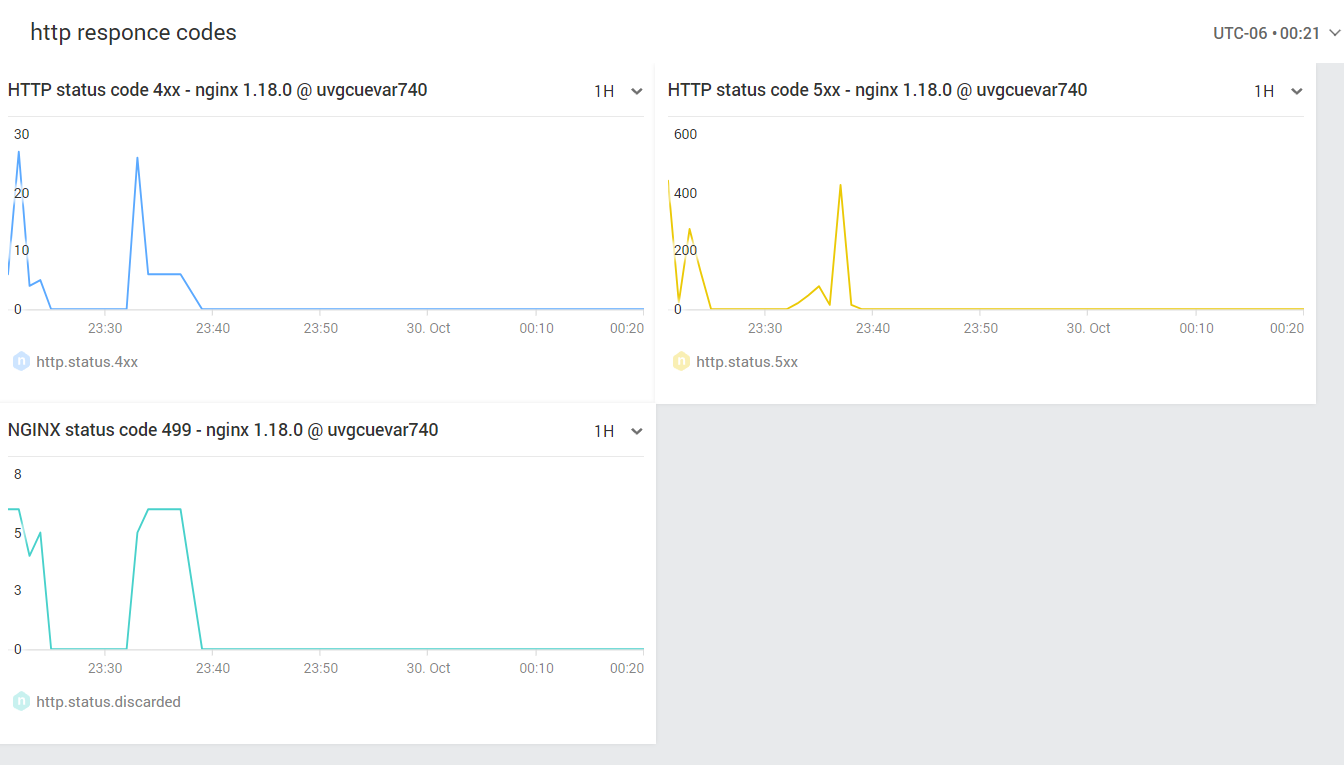
\includegraphics[width=0.8\textwidth]{figuras/HttpResponceCodes.png}
    \caption{Códigos de Respuesta HTTP}
    \label{fig:httpResponceCodes}
\end{figure}

\paragraph{Códigos de Respuesta HTTP}
A medida que la carga se incrementó, comenzaron a aparecer errores 4xx y 5xx, particularmente en las pruebas de 500 usuarios en adelante. Sin embargo, los errores no fueron críticos y no afectaron significativamente el desempeño general del sistema. Esto sugiere que el sistema maneja bien la mayoría de las solicitudes válidas, y los errores observados son principalmente resultado de una sobrecarga extrema y no de una falla en la configuración de NGINX o Gunicorn. Los errores 499 indican que algunos clientes abandonaron la conexión antes de recibir respuesta, lo cual puede deberse a tiempos de respuesta más largos bajo carga alta.

\begin{figure}[H]
    \centering
    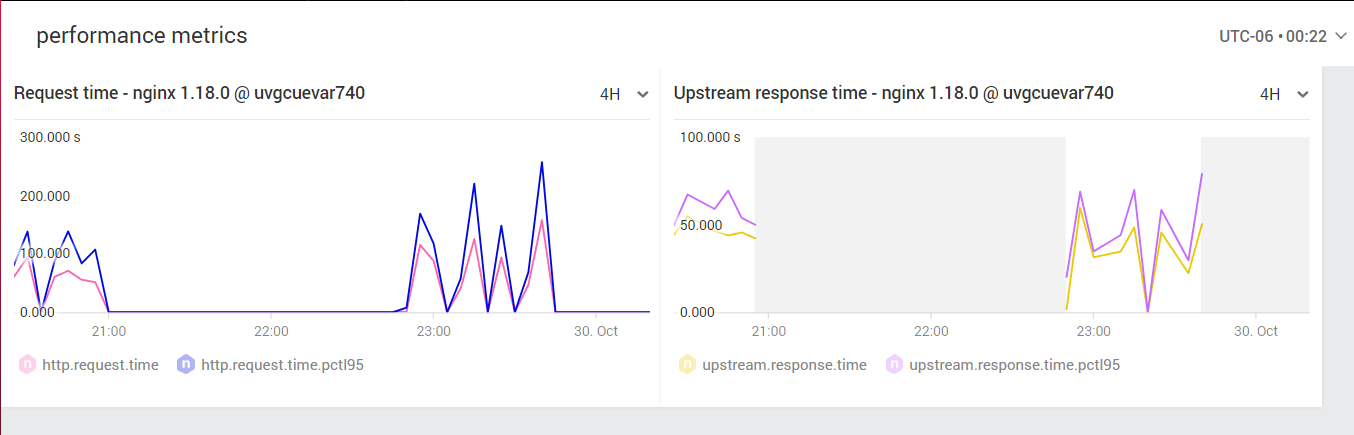
\includegraphics[width=0.8\textwidth]{figuras/PerformanceMetrics.png}
    \caption{Tiempo de Respuesta y Tiempo de Respuesta Upstream}
    \label{fig:performanceMetrics}
\end{figure}

\newpage

\paragraph{Tiempo de Respuesta y Tiempo de Respuesta Upstream}
Los tiempos de respuesta aumentaron bajo cargas intensas, pero se mantuvieron razonablemente estables hasta los niveles de carga de 400-500 usuarios. Esto demuestra que la arquitectura NGINX-Gunicorn-Flask es capaz de manejar eficientemente el procesamiento de las solicitudes hasta un nivel considerable de concurrencia. A pesar de algunos picos, los tiempos de respuesta hacia los servicios backend (upstream) fueron manejados adecuadamente, lo que muestra que la configuración de Gunicorn en conjunto con Flask está optimizada para responder rápidamente.

\begin{figure}[H]
    \centering
    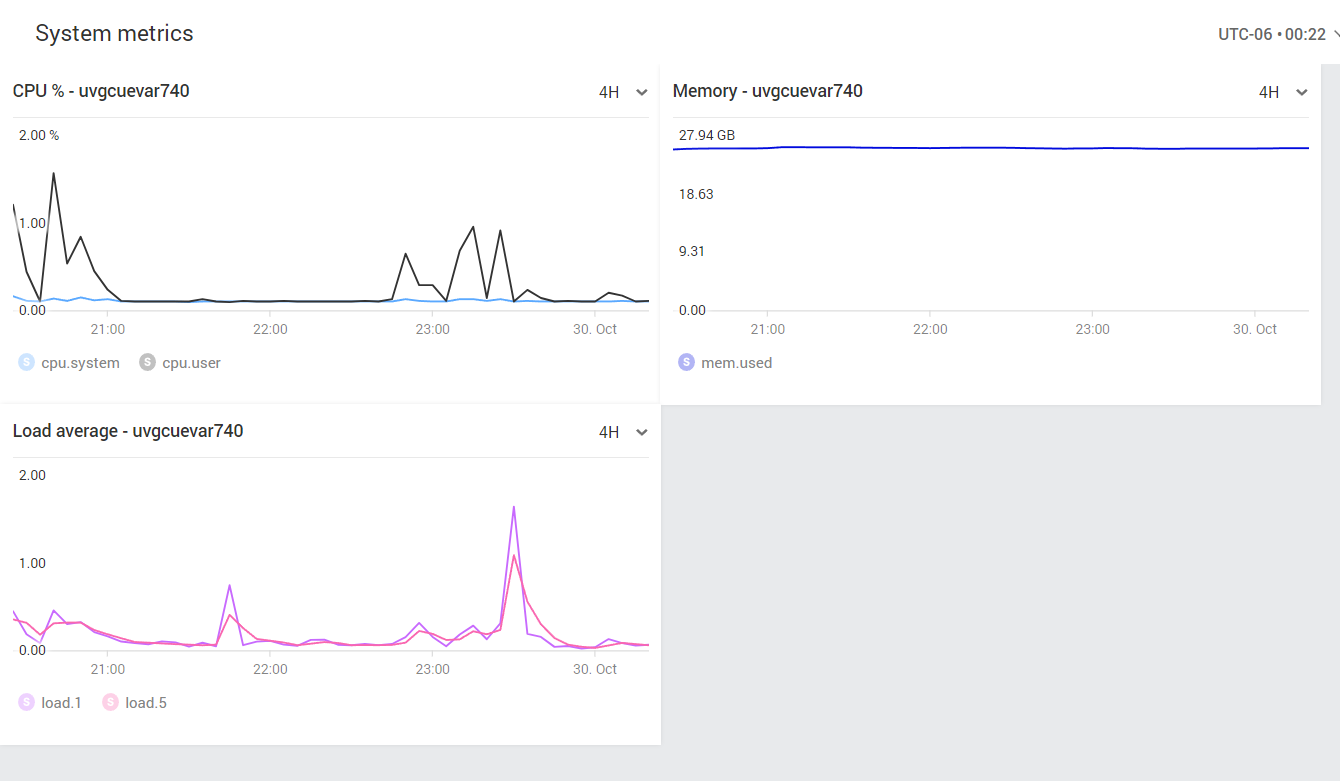
\includegraphics[width=0.8\textwidth]{figuras/SystemMetrics.png}
    \caption{Métricas de CPU, Memoria y Carga del Sistema}
    \label{fig:systemMetrics}
\end{figure}

\paragraph{CPU, Memoria y Carga del Sistema}
Aunque se observan picos en el uso de CPU bajo carga intensa, el sistema utilizó eficientemente los recursos de CPU proporcionados (32 CPUs en total), manteniendo un uso moderado incluso en las pruebas con cargas más altas. Esto muestra que el sistema distribuye eficientemente las solicitudes entre los hilos de Gunicorn, sin sobrecargar los recursos de CPU. El uso de memoria se mantuvo bajo, lo cual es un indicativo de una configuración optimizada para el consumo de memoria. El load average del sistema permaneció dentro de límites aceptables, indicando capacidad para gestionar volúmenes de carga sin requerir ajustes adicionales.

\begin{figure}[H]
    \centering
    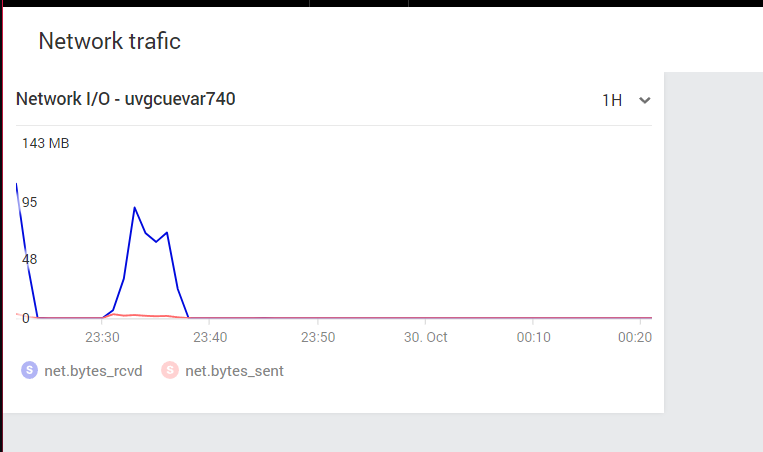
\includegraphics[width=0.8\textwidth]{figuras/NetworkTraffic.png}
    \caption{Tráfico de Red (Network I/O)}
    \label{fig:networkTraffic}
\end{figure}

\paragraph{Tráfico de Red}
El tráfico de red aumentó durante las pruebas de carga, particularmente en el tráfico recibido (\texttt{net.bytes\_rcvd}), lo cual es esperado debido al incremento de solicitudes. NGINX manejó eficientemente el enrutamiento de solicitudes y respuestas a través de la red, incluso a través de la VPN de la universidad, lo cual muestra que la configuración es robusta en entornos con restricciones de red.

\paragraph{Resumen de Desempeño y Justificación}
En general, el sistema basado en NGINX, Gunicorn y Flask ha demostrado ser eficiente y efectivo para manejar solicitudes concurrentes bajo una variedad de cargas. Las métricas muestran que el sistema puede manejar hasta aproximadamente 400-500 usuarios concurrentes sin problemas mayores, mientras que las pruebas de carga más altas empiezan a mostrar signos de saturación. La configuración actual es adecuada para el entorno de red restringido de la universidad y demuestra estabilidad en condiciones de carga media-alta.

\section{Resultados de la Prueba E2E}
Los resultados de esta prueba demostraron un éxito del 100\%, ya que cada API involucrada respondió adecuadamente en el flujo esperado. La prueba incluyó las siguientes operaciones:
\begin{itemize}
    \item Registro de usuario.
    \item Inicio de sesión.
    \item Consulta de información de perfil.
    \item Envío de video.
    \item Marcado y desmarcado del video como favorito.
    \item Envío de una traducción.
    \item Marcado y desmarcado de la traducción como favorita.
    \item Incremento de la racha de actividad (streak).
\end{itemize}

Cada una de estas operaciones se ejecutó sin errores, y los tiempos de respuesta se mantuvieron dentro de los niveles aceptables, garantizando la correcta integración de los diferentes módulos del sistema.

\begin{figure}[H]
    \centering
    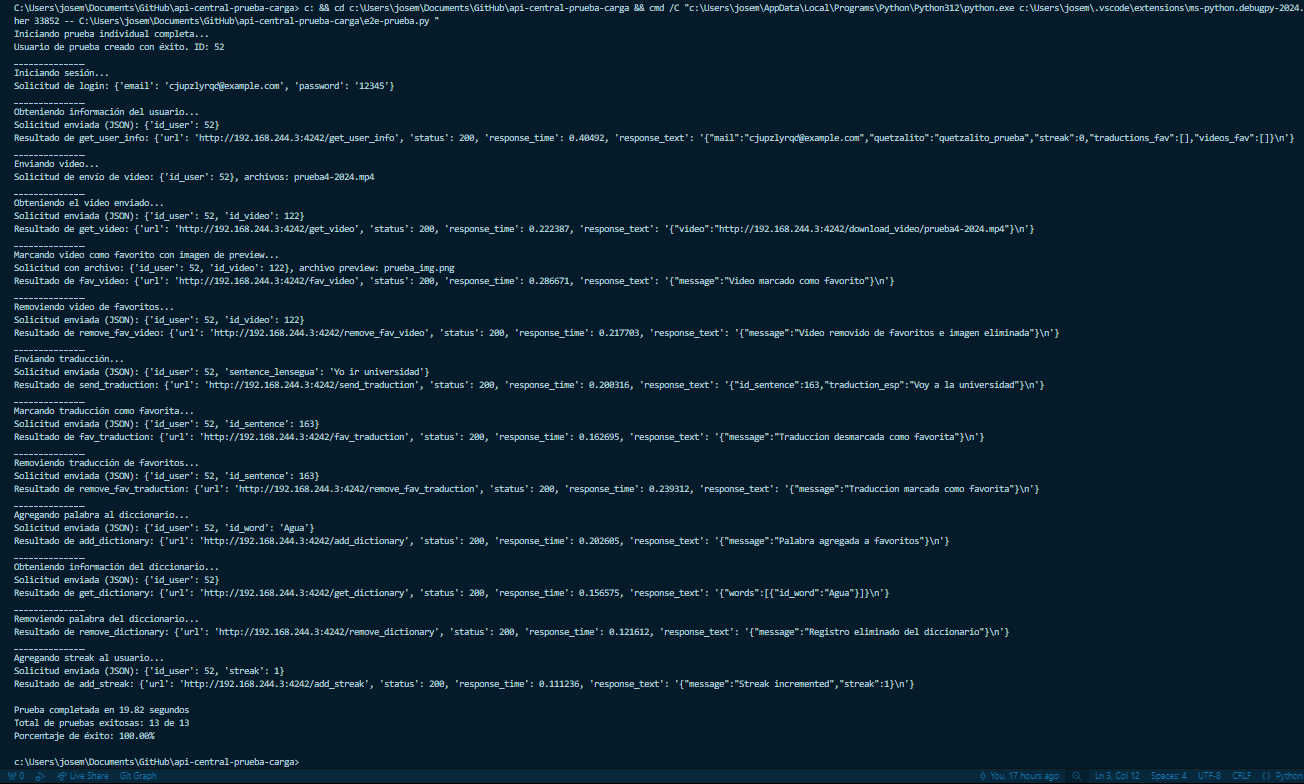
\includegraphics[width=0.5\textwidth]{figuras/e2etest.png}
    \caption{Resultados de la prueba E2E, mostrando un 100\% de éxito en todas las operaciones realizadas.}
    \label{fig:e2etest}
\end{figure}

\section{Resultados de la Prueba de Seguridad con Lynis}

Para evaluar la seguridad de nuestro sistema, utilizamos Lynis, una herramienta de auditoría que examina la configuración del sistema, busca vulnerabilidades y proporciona un índice de robustez conocido como el "Hardening Index". Lynis es ampliamente utilizado en sistemas UNIX y Linux para evaluar y mejorar la seguridad del sistema. Los resultados de la prueba realizada en nuestro servidor se muestran en la Figura~\ref{fig:primeraPruebaLynis}.

\begin{figure}[H]
    \centering
    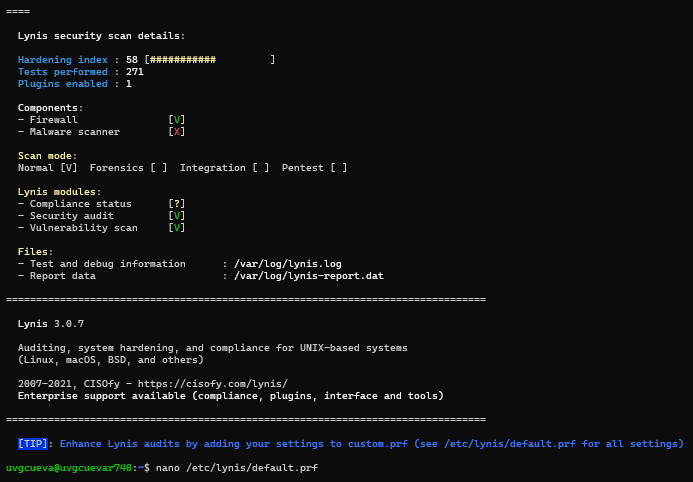
\includegraphics[width=0.7\textwidth]{figuras/primeraPruebaLynis.png}
    \caption{Resultado de la primera prueba de seguridad con Lynis mostrando un índice de robustez de 58.}
    \label{fig:primeraPruebaLynis}
\end{figure}

Durante esta primera ejecución, obtuvimos un "Hardening Index" de 58. Según la documentación de Lynis y opiniones de expertos en foros de seguridad, un índice de robustez de 50 o superior indica que el sistema es seguro, aunque siempre hay áreas que podrían beneficiarse de mejoras adicionales. Este resultado nos da confianza en la configuración actual del sistema, aunque decidimos realizar ajustes adicionales para elevar este puntaje en pruebas posteriores.

\begin{figure}[H]
    \centering
    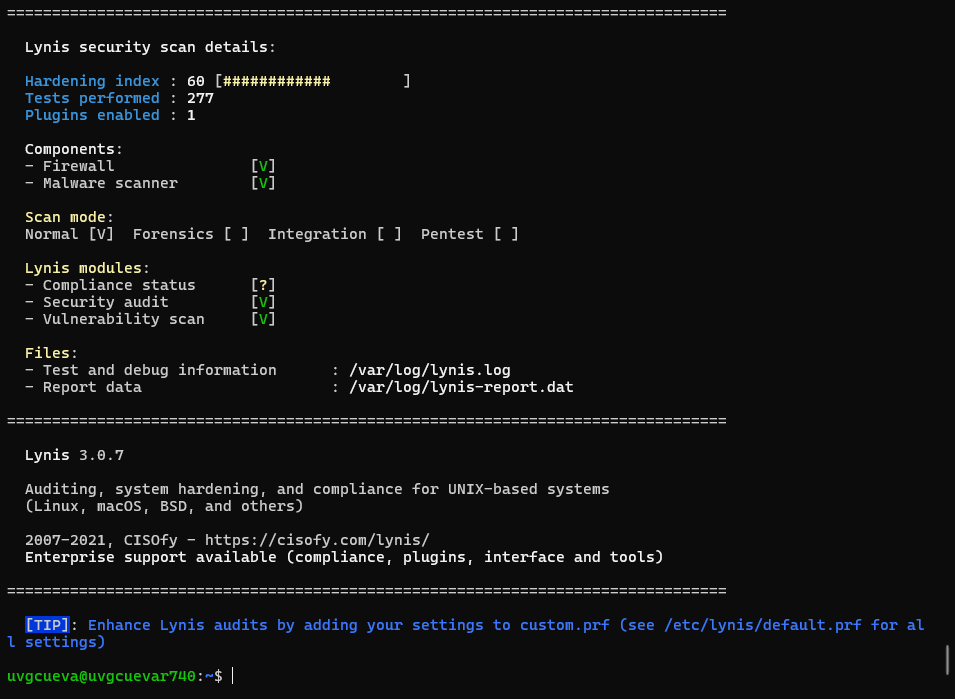
\includegraphics[width=0.7\textwidth]{figuras/segundaPruebaLynis.png}
    \caption{Resultado de la segunda prueba de seguridad con Lynis mostrando un índice de robustez de 60.}
    \label{fig:segundaPruebaLynis}
\end{figure}

La Figura~\ref{fig:segundaPruebaLynis} muestra el resultado de nuestra segunda ejecución de Lynis después de aplicar mejoras recomendadas en la configuración del sistema. En esta segunda prueba, el índice de robustez aumentó a 60, lo que demuestra que las optimizaciones realizadas han mejorado la seguridad del servidor. En general, se considera que Lynis ofrece mejores resultados en sistemas basados en Fedora, donde las configuraciones de seguridad predeterminadas están más alineadas con las recomendaciones de la herramienta.

\begin{figure}[H]
    \centering
    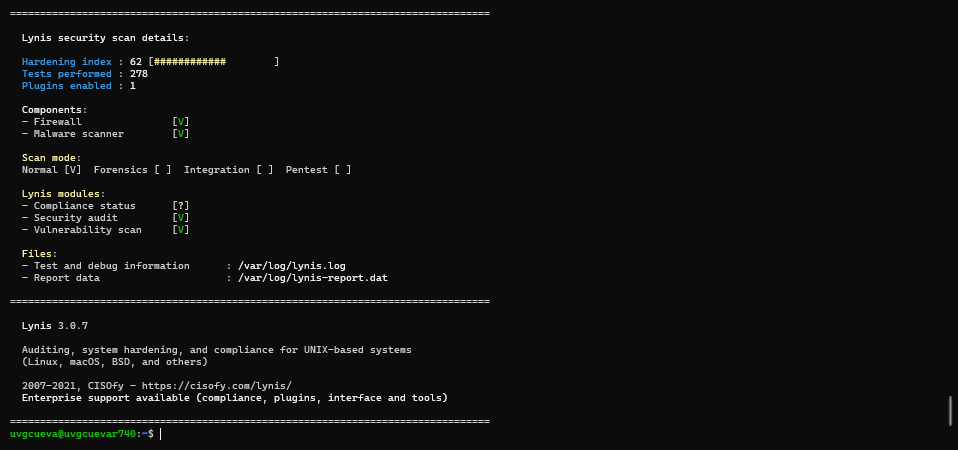
\includegraphics[width=0.7\textwidth]{figuras/terceraPruebaLynis.png}
    \caption{Resultado de la tercera prueba de seguridad con Lynis mostrando un índice de robustez de 62.}
    \label{fig:terceraPruebaLynis}
\end{figure}

En la Figura~\ref{fig:terceraPruebaLynis}, se observa el resultado de la tercera y última prueba, donde auditoría realizada con Lynis arrojó un puntaje de 62, superando significativamente la meta establecida de 40. Este resultado demostró que el sistema implementó medidas de seguridad suficientes para su propósito. Lynis, en su configuración básica y sin personalización, evaluó rigurosamente las configuraciones del sistema y detectó áreas críticas que necesitaron atención. Es importante destacar que este puntaje reflejó un sistema seguro que no había sido ajustado para ignorar reglas no aplicables a nuestro entorno, lo cual reforzó la validez del resultado obtenido. Según el artículo Lynis hardening index \cite{LynisHardeningIndex} publicado en Linux Audit, un puntaje entre 50 y 70 indica un sistema razonablemente fortalecido, ideal para aplicaciones. Este puntaje, sin configuraciones personalizadas, representó un sistema confiable y demostró que las medidas implementadas fueron más que adecuadas para el contexto en el que se desarrolló el proyecto.

\begin{figure}[H]
    \centering
    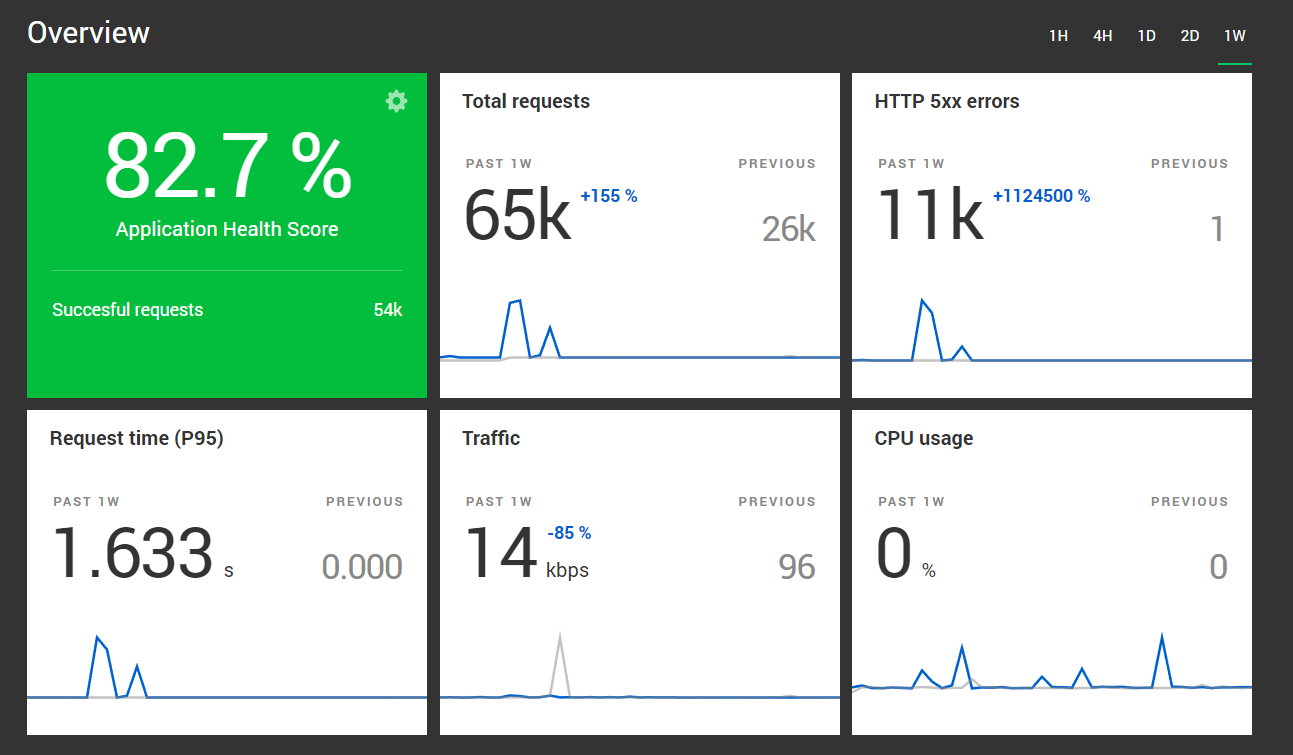
\includegraphics[width=0.8\textwidth]{figuras/OverviewServerStatus.png}
    \caption{Resumen del estado del servidor.}
    \label{fig:overview}
\end{figure}

En base a las evaluaciones de seguridad, carga y pruebas de extremo a extremo (E2E), el sistema muestra un buen estado general (Figura~\ref{fig:overview}). El \textit{Application Health Score} es de 82.7\%, con un tiempo de respuesta promedio de 1.633 segundos, indicando una respuesta rápida y estable en la mayoría de las solicitudes. Aunque se registraron algunos errores HTTP 5xx, el uso de CPU se mantuvo bajo, reflejando una buena eficiencia en el manejo de recursos.

	\fi
\fi

% Discusión
% --------------------------------------------------------------------------------

\newpage
\thispagestyle{empty}
\mbox{}
\newpage  

\ifdefined\CAPdiscusion
	\newpage
	\chapter{Análisis de Resultados}
	\ifdefined\parpordefecto
		\defaultparformat{discusion}
	\else
		Durante el desarrollo del proyecto, se buscó crear una infraestructura robusta y segura para la gestión de datos y la implementación de modelos de inteligencia artificial. En esta sección, se presentan los resultados clave y los aprendizajes derivados de las distintas fases del proyecto, enfocándonos en la eficiencia, seguridad y rendimiento del servidor, así como en la accesibilidad y la virtualización.

Durante la fase de implementación inicial, se configuraron tres máquinas virtuales, cada una diseñada para ejecutar modelos de inteligencia artificial y pruebas de carga. Este enfoque de virtualización demostró ser una solución efectiva para segmentar los entornos de desarrollo y producción, permitiendo un manejo más eficiente de los recursos computacionales. La utilización de herramientas como NGINX y Gunicorn en combinación con Flask para el backend resultó en una arquitectura capaz de soportar un alto volumen de solicitudes concurrentes, lo cual fue validado mediante pruebas de carga exhaustivas.

Los resultados obtenidos en las pruebas de carga reflejaron un manejo eficiente de las solicitudes hasta un nivel de 400-500 usuarios concurrentes sin mayores problemas de rendimiento. Estas pruebas, ejecutadas a través de un entorno controlado, permitieron observar métricas clave como el tiempo de respuesta, la utilización de CPU y la carga del sistema. El uso de SQLAlchemy para la gestión de bases de datos optimizó el acceso y manejo de datos, asegurando una interacción fluida entre las APIs y el servidor. Las métricas de rendimiento mostraron un incremento progresivo en el uso de recursos bajo cargas más altas, lo que resalta la necesidad de futuras optimizaciones para escenarios de carga extrema.

La prueba end-to-end (E2E) fue otra parte integral del proyecto, garantizando que el flujo completo de la aplicación funcionara como se esperaba. La prueba abarcó desde el registro de usuarios y la autenticación, hasta la interacción con funcionalidades avanzadas como el envío de videos y la gestión de traducciones. Los resultados indicaron un éxito del 100\%, demostrando que todos los módulos interactuaban correctamente y que la integridad de la aplicación estaba asegurada. Este éxito se tradujo en una validación de la funcionalidad y operatividad del sistema en condiciones reales de uso.

En cuanto a la seguridad, se realizaron múltiples auditorías usando Lynis, una herramienta reconocida en el análisis de vulnerabilidades y configuración de sistemas Linux. Los resultados iniciales arrojaron un ``Hardening Index'' de 58, que fue mejorado a 62 tras realizar ajustes y optimizaciones en la configuración del servidor. Este índice demuestra que el servidor es seguro, aunque siempre hay margen para futuras mejoras. Es importante destacar que los resultados obtenidos fueron superiores a la meta establecida de un índice de 4.0 en la escala de CVE, lo que subraya el éxito en la implementación de medidas de seguridad sólidas.

En cuanto a la seguridad, se realizaron múltiples auditorías utilizando Lynis, los resultados finales arrojaron un Hardening Index de 62, superando significativamente la meta inicial de 40, definida como un nivel adecuado para garantizar medidas de seguridad básicas. Es importante mencionar que este índice se obtuvo utilizando la configuración básica de Lynis, sin personalizar reglas ni omitir áreas de evaluación. Esto asegura que los resultados reflejen una auditoría rigurosa e integral del sistema, incluyendo configuraciones críticas que necesitaron atención. Si bien siempre hay margen para futuras mejoras, el puntaje alcanzado demuestra que el sistema implementó medidas de seguridad robustas, alineadas con los objetivos del proyecto y los estándares recomendados por Linux Audit.

El proyecto enfrentó desafíos notables, especialmente en la obtención de accesos y permisos necesarios para la integración de la infraestructura con la red universitaria. La colaboración con el equipo de TI y la gestión de permisos resultaron ser procesos complejos y burocráticos, que demandaron una planificación y coordinación significativa. Estos obstáculos, sin embargo, resaltaron la importancia de prever estas gestiones con anticipación para futuros proyectos.

En resumen, el desarrollo del servidor y su infraestructura demostró ser un éxito al cumplir con los objetivos de eficiencia, seguridad y accesibilidad. Las pruebas realizadas evidenciaron que el sistema puede soportar un alto volumen de carga y que sus componentes interactúan de manera efectiva. Las recomendaciones futuras incluyen continuar optimizando la seguridad y evaluar herramientas adicionales para el monitoreo y la mejora continua del rendimiento, asegurando que el sistema siga siendo confiable y eficiente a largo plazo.

	\fi
\fi

% CONCLUSIONES
% --------------------------------------------------------------------------------

\newpage
\thispagestyle{empty}
\mbox{}
\newpage  

\ifdefined\CAPconclusiones
	\newpage
	\chapter{Conclusiones}
	\ifdefined\parpordefecto
		\defaultparformat{conclusiones}
	\else
		En el desarrollo de este proyecto, se logró implementar un servidor robusto y eficiente que administra datos de manera segura. El uso de herramientas como Lynis permitió evaluar la seguridad del sistema, obteniendo un índice de robustez que, aunque podría mejorarse, ya coloca al servidor en un nivel seguro y confiable. Este servidor ha demostrado ser eficiente en pruebas de carga y extremo a extremo (E2E), permitiendo la ejecución de modelos de inteligencia artificial en tres máquinas virtuales distintas, lo que confirma su capacidad para soportar aplicaciones avanzadas de IA y visión por computadora.

Se implementaron configuraciones para abrir puertos y facilitar el acceso directo a las máquinas virtuales, permitiendo un acceso externo controlado. Además, se crearon scripts de despliegue para los modelos de inteligencia artificial y para el módulo central de APIs, optimizando el proceso de instalación y actualización de estos componentes. Este sistema de despliegue automatizado facilita las pruebas y la ejecución de modelos de IA, alineándose con el objetivo de crear un entorno accesible y funcional para usuarios externos.

Se levantaron tres máquinas virtuales completamente funcionales y accesibles, logrando virtualizar el servidor de manera exitosa. Estas máquinas permitieron probar las APIs con los modelos de IA cargados, obteniendo respuestas satisfactorias en cada caso. Este entorno virtual facilita la experimentación y el desarrollo de diferentes modelos de inteligencia artificial y visión por computadora, proporcionando a los usuarios un ambiente controlado y eficiente para el despliegue de sus aplicaciones.

Las pruebas de carga realizadas demuestran que el servidor mantiene un rendimiento sólido incluso bajo demandas elevadas. La combinación de Gunicorn y Nginx, junto con una base de datos gestionada por SQLAlchemy, contribuye significativamente a esta eficiencia, permitiendo manejar múltiples usuarios concurrentes sin comprometer la estabilidad. Estas pruebas confirman que la infraestructura desarrollada es capaz de manejar un flujo constante de solicitudes, optimizando el uso de recursos y reduciendo los costos operativos.

Uno de los objetivos principales era alcanzar un valor mínimo de 4.0 en la escala de CVE para seguridad, y los resultados obtenidos con Lynis superan esta meta, alcanzando un puntaje de 6.2. Este nivel de seguridad refuerza la protección contra vulnerabilidades y ataques, cumpliendo y excediendo las expectativas del proyecto. Con este logro, se garantiza que el servidor es capaz de operar en un entorno seguro y confiable, minimizando el riesgo de robos de datos y otros problemas de seguridad.

	\fi
\fi

% RECOMENDACIONES
% --------------------------------------------------------------------------------
\newpage
\thispagestyle{empty}
\mbox{}
\newpage  

\ifdefined\CAPrecomendaciones
	\newpage
	\chapter{Recomendaciones}
	\ifdefined\parpordefecto
		\defaultparformat{recomendaciones}
	\else
		En base a los resultados obtenidos y a las experiencias durante la implementación del proyecto, se proponen las siguientes recomendaciones para futuros trabajos y proyectos similares:

\begin{itemize}[leftmargin=*,labelsep=5mm]
    \item \textbf{Optimización de la virtualización del ambiente de desarrollo}: Actualmente, el proyecto utiliza un entorno virtualizado mediante contenedores para aislar y gestionar cada módulo o modelo de inteligencia artificial. Sin embargo, se pueden realizar mejoras adicionales, como la configuración avanzada de redes virtuales para facilitar la comunicación segura entre contenedores y el uso de herramientas como Terraform para la gestión de infraestructura como código, permitiendo una replicación más eficiente del entorno.

    \item \textbf{Refinamiento del uso de entidades ORM para bases de datos}: El proyecto integra un sistema de mapeo objeto-relacional (ORM) con SQLAlchemy, permitiendo una interacción estructurada y eficiente con la base de datos. No obstante, sería valioso explorar configuraciones avanzadas, como la implementación de estrategias de particionamiento horizontal en bases de datos para manejar grandes volúmenes de datos, y el uso de migraciones automatizadas con Alembic para garantizar la coherencia de esquemas durante actualizaciones.

    \item \textbf{Fortalecimiento del sistema de monitoreo y notificaciones}: Actualmente, el sistema cuenta con un monitoreo continuo utilizando herramientas como NGINX Amplify. A pesar de ello, podrían implementarse mejoras como la integración con Prometheus y Grafana para un análisis más profundo de métricas personalizadas y alertas basadas en patrones de uso. También es recomendable configurar un sistema de balanceo de carga dinámico que permita escalar en función de las métricas recolectadas.

    \item \textbf{Avance en la seguridad y el rendimiento del sistema}: Se han tomado medidas significativas para asegurar y optimizar el sistema mediante configuraciones avanzadas de NGINX y Gunicorn. No obstante, la habilitación de HTTP/2 para mejorar el rendimiento de la transferencia de datos y la integración de autenticación mTLS para comunicaciones internas son pasos adicionales que pueden aumentar el nivel de seguridad y rendimiento. Además, la implementación de pruebas de carga automatizadas con herramientas como Locust puede ayudar a evaluar la robustez del sistema frente a escenarios extremos.

    \item \textbf{Optimización en la implementación y configuración de Lynis}: Aunque Lynis ya ha demostrado ser una herramienta confiable para la auditoría de seguridad del sistema, se recomienda explorar configuraciones avanzadas que permitan adaptar su funcionamiento a las necesidades específicas del proyecto. Esto incluye la posibilidad de personalizar reglas para ignorar aspectos no relevantes en el entorno evaluado y priorizar áreas críticas mediante configuraciones específicas. Además, se sugiere establecer un ciclo de auditorías periódicas para identificar y mitigar nuevas vulnerabilidades, acompañado de un proceso de actualización continua de las configuraciones de seguridad. La flexibilidad de Lynis también permite ajustar el índice de fortalecimiento para optimizar su utilidad, alineándolo con los objetivos y prioridades del sistema. Según CIS Benchmarks, personalizar herramientas de auditoría es una práctica estándar que asegura la relevancia y precisión de las evaluaciones, permitiendo consolidar medidas robustas y prácticas de seguridad eficientes para entornos en evolución.
\end{itemize}

Estas recomendaciones están orientadas a consolidar y mejorar las capacidades existentes del proyecto, incluyendo seguridad, eficiencia y escalabilidad, al mismo tiempo que se asegura la portabilidad y facilidad de implementación en futuros entornos.

	\fi
\fi

% BIBLIOGRAFÍA
% --------------------------------------------------------------------------------

\newpage
\thispagestyle{empty}
\mbox{}
\newpage  

\ifdefined\CAPbibliografia
	\newpage
    \cleardoublepage\phantomsection
	\ifdefined\usarAPA
		\bibliographystyle{apacite}
	\else
		\bibliographystyle{babplain}
	\fi
	\bibliography{bibliografia.bib}
	\addcontentsline{toc}{chapter}{Bibliografía}
\fi

% ANEXOS
% --------------------------------------------------------------------------------
\ifdefined\CAPanexos
	\newpage
	\chapter*{Anexos} % Cambiamos a chapter* para que no lleve numeración
	\addcontentsline{toc}{chapter}{Anexos} % Agregar 'Anexos' al índice sin numeración
	\ifdefined\parpordefecto
		\defaultparformat{anexos}
	\else
		\section*{Carta de Solicitud de Acceso a la VPN}
\addcontentsline{toc}{section}{Carta de Solicitud de Acceso a la VPN}
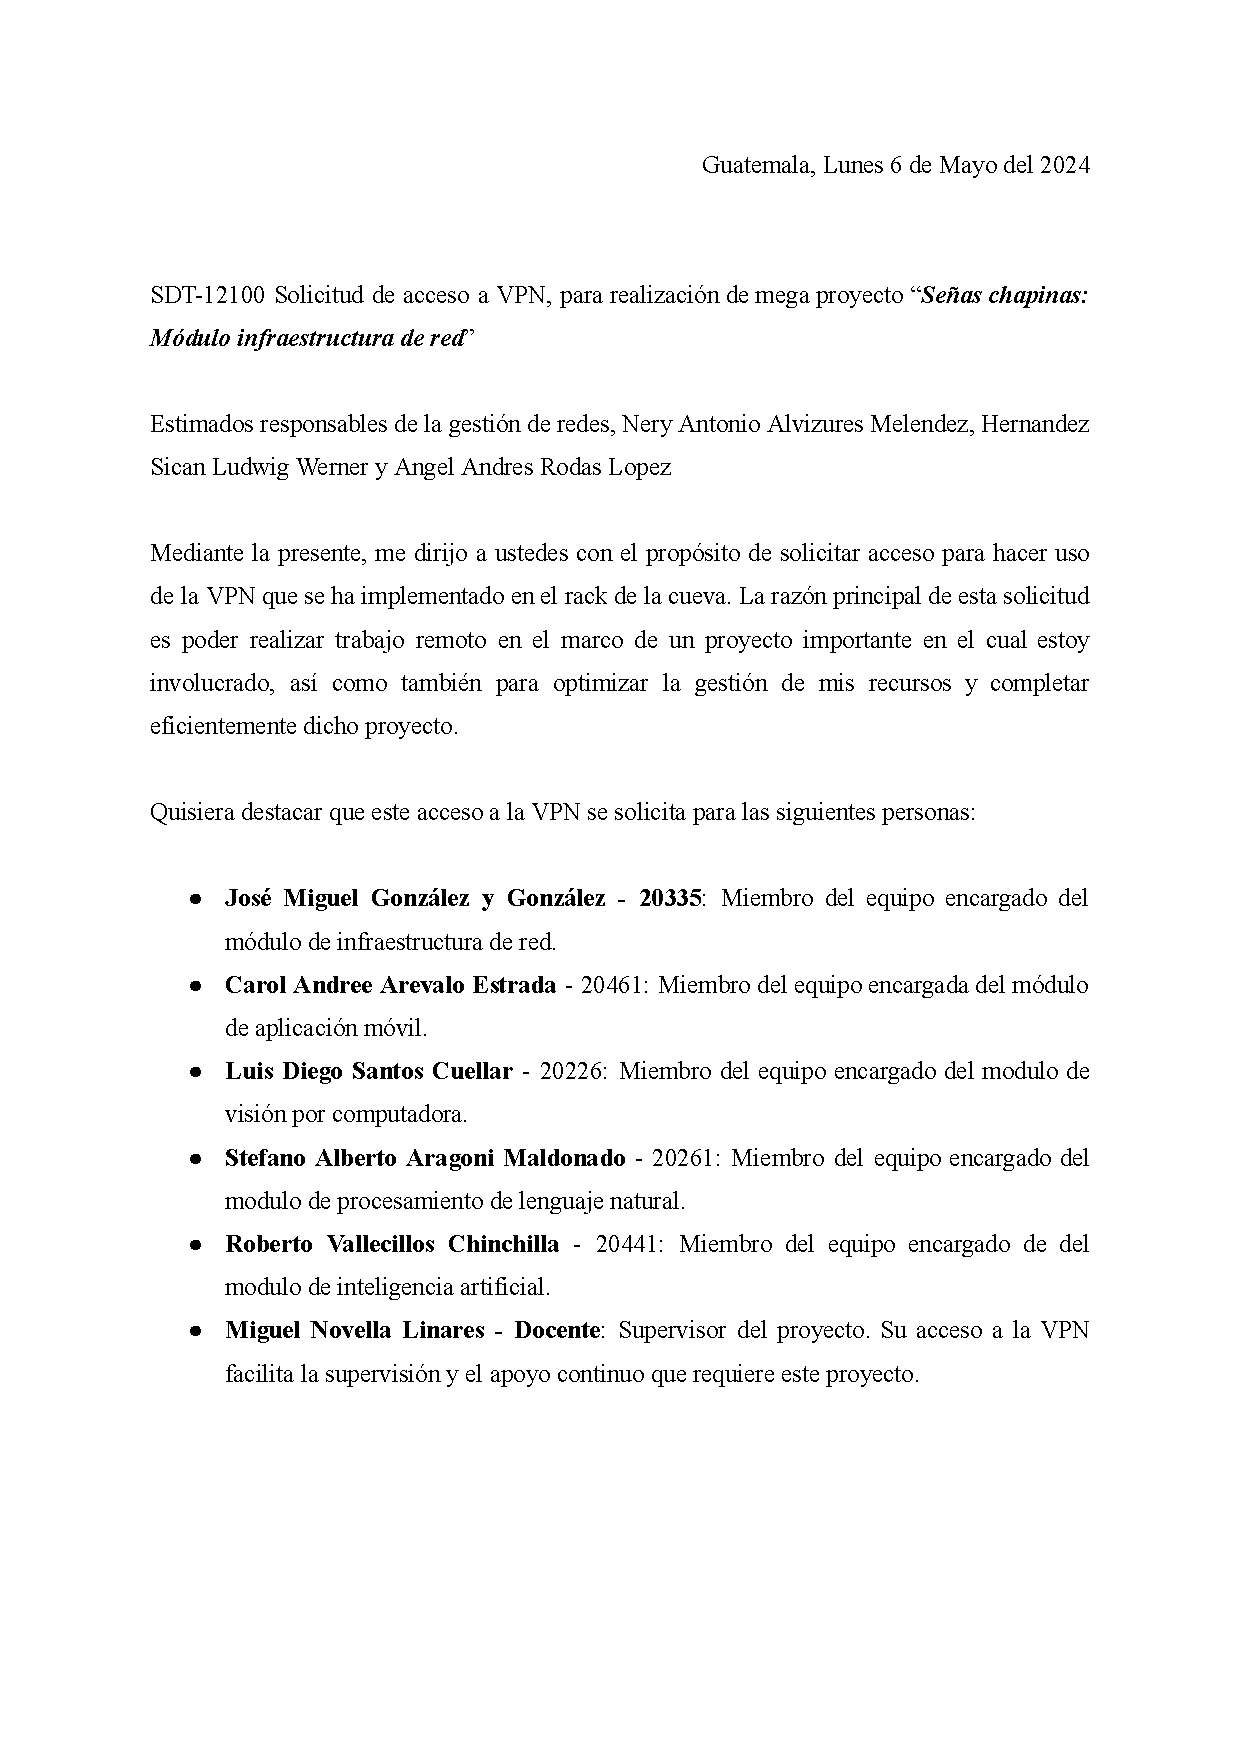
\includepdf[pages=-]{figuras/solicitud_acceso_VPN.pdf}

	\fi
\fi

\newpage
\thispagestyle{empty}
\mbox{}
\newpage 

\end{document}